% Options for packages loaded elsewhere
\PassOptionsToPackage{unicode}{hyperref}
\PassOptionsToPackage{hyphens}{url}
\PassOptionsToPackage{dvipsnames,svgnames,x11names}{xcolor}
%
\documentclass[
  letterpaper,
  DIV=11,
  numbers=noendperiod]{scrreprt}

\usepackage{amsmath,amssymb}
\usepackage{lmodern}
\usepackage{iftex}
\ifPDFTeX
  \usepackage[T1]{fontenc}
  \usepackage[utf8]{inputenc}
  \usepackage{textcomp} % provide euro and other symbols
\else % if luatex or xetex
  \usepackage{unicode-math}
  \defaultfontfeatures{Scale=MatchLowercase}
  \defaultfontfeatures[\rmfamily]{Ligatures=TeX,Scale=1}
\fi
% Use upquote if available, for straight quotes in verbatim environments
\IfFileExists{upquote.sty}{\usepackage{upquote}}{}
\IfFileExists{microtype.sty}{% use microtype if available
  \usepackage[]{microtype}
  \UseMicrotypeSet[protrusion]{basicmath} % disable protrusion for tt fonts
}{}
\makeatletter
\@ifundefined{KOMAClassName}{% if non-KOMA class
  \IfFileExists{parskip.sty}{%
    \usepackage{parskip}
  }{% else
    \setlength{\parindent}{0pt}
    \setlength{\parskip}{6pt plus 2pt minus 1pt}}
}{% if KOMA class
  \KOMAoptions{parskip=half}}
\makeatother
\usepackage{xcolor}
\setlength{\emergencystretch}{3em} % prevent overfull lines
\setcounter{secnumdepth}{5}
% Make \paragraph and \subparagraph free-standing
\ifx\paragraph\undefined\else
  \let\oldparagraph\paragraph
  \renewcommand{\paragraph}[1]{\oldparagraph{#1}\mbox{}}
\fi
\ifx\subparagraph\undefined\else
  \let\oldsubparagraph\subparagraph
  \renewcommand{\subparagraph}[1]{\oldsubparagraph{#1}\mbox{}}
\fi

\usepackage{color}
\usepackage{fancyvrb}
\newcommand{\VerbBar}{|}
\newcommand{\VERB}{\Verb[commandchars=\\\{\}]}
\DefineVerbatimEnvironment{Highlighting}{Verbatim}{commandchars=\\\{\}}
% Add ',fontsize=\small' for more characters per line
\usepackage{framed}
\definecolor{shadecolor}{RGB}{241,243,245}
\newenvironment{Shaded}{\begin{snugshade}}{\end{snugshade}}
\newcommand{\AlertTok}[1]{\textcolor[rgb]{0.68,0.00,0.00}{#1}}
\newcommand{\AnnotationTok}[1]{\textcolor[rgb]{0.37,0.37,0.37}{#1}}
\newcommand{\AttributeTok}[1]{\textcolor[rgb]{0.40,0.45,0.13}{#1}}
\newcommand{\BaseNTok}[1]{\textcolor[rgb]{0.68,0.00,0.00}{#1}}
\newcommand{\BuiltInTok}[1]{\textcolor[rgb]{0.00,0.23,0.31}{#1}}
\newcommand{\CharTok}[1]{\textcolor[rgb]{0.13,0.47,0.30}{#1}}
\newcommand{\CommentTok}[1]{\textcolor[rgb]{0.37,0.37,0.37}{#1}}
\newcommand{\CommentVarTok}[1]{\textcolor[rgb]{0.37,0.37,0.37}{\textit{#1}}}
\newcommand{\ConstantTok}[1]{\textcolor[rgb]{0.56,0.35,0.01}{#1}}
\newcommand{\ControlFlowTok}[1]{\textcolor[rgb]{0.00,0.23,0.31}{#1}}
\newcommand{\DataTypeTok}[1]{\textcolor[rgb]{0.68,0.00,0.00}{#1}}
\newcommand{\DecValTok}[1]{\textcolor[rgb]{0.68,0.00,0.00}{#1}}
\newcommand{\DocumentationTok}[1]{\textcolor[rgb]{0.37,0.37,0.37}{\textit{#1}}}
\newcommand{\ErrorTok}[1]{\textcolor[rgb]{0.68,0.00,0.00}{#1}}
\newcommand{\ExtensionTok}[1]{\textcolor[rgb]{0.00,0.23,0.31}{#1}}
\newcommand{\FloatTok}[1]{\textcolor[rgb]{0.68,0.00,0.00}{#1}}
\newcommand{\FunctionTok}[1]{\textcolor[rgb]{0.28,0.35,0.67}{#1}}
\newcommand{\ImportTok}[1]{\textcolor[rgb]{0.00,0.46,0.62}{#1}}
\newcommand{\InformationTok}[1]{\textcolor[rgb]{0.37,0.37,0.37}{#1}}
\newcommand{\KeywordTok}[1]{\textcolor[rgb]{0.00,0.23,0.31}{#1}}
\newcommand{\NormalTok}[1]{\textcolor[rgb]{0.00,0.23,0.31}{#1}}
\newcommand{\OperatorTok}[1]{\textcolor[rgb]{0.37,0.37,0.37}{#1}}
\newcommand{\OtherTok}[1]{\textcolor[rgb]{0.00,0.23,0.31}{#1}}
\newcommand{\PreprocessorTok}[1]{\textcolor[rgb]{0.68,0.00,0.00}{#1}}
\newcommand{\RegionMarkerTok}[1]{\textcolor[rgb]{0.00,0.23,0.31}{#1}}
\newcommand{\SpecialCharTok}[1]{\textcolor[rgb]{0.37,0.37,0.37}{#1}}
\newcommand{\SpecialStringTok}[1]{\textcolor[rgb]{0.13,0.47,0.30}{#1}}
\newcommand{\StringTok}[1]{\textcolor[rgb]{0.13,0.47,0.30}{#1}}
\newcommand{\VariableTok}[1]{\textcolor[rgb]{0.07,0.07,0.07}{#1}}
\newcommand{\VerbatimStringTok}[1]{\textcolor[rgb]{0.13,0.47,0.30}{#1}}
\newcommand{\WarningTok}[1]{\textcolor[rgb]{0.37,0.37,0.37}{\textit{#1}}}

\providecommand{\tightlist}{%
  \setlength{\itemsep}{0pt}\setlength{\parskip}{0pt}}\usepackage{longtable,booktabs,array}
\usepackage{calc} % for calculating minipage widths
% Correct order of tables after \paragraph or \subparagraph
\usepackage{etoolbox}
\makeatletter
\patchcmd\longtable{\par}{\if@noskipsec\mbox{}\fi\par}{}{}
\makeatother
% Allow footnotes in longtable head/foot
\IfFileExists{footnotehyper.sty}{\usepackage{footnotehyper}}{\usepackage{footnote}}
\makesavenoteenv{longtable}
\usepackage{graphicx}
\makeatletter
\def\maxwidth{\ifdim\Gin@nat@width>\linewidth\linewidth\else\Gin@nat@width\fi}
\def\maxheight{\ifdim\Gin@nat@height>\textheight\textheight\else\Gin@nat@height\fi}
\makeatother
% Scale images if necessary, so that they will not overflow the page
% margins by default, and it is still possible to overwrite the defaults
% using explicit options in \includegraphics[width, height, ...]{}
\setkeys{Gin}{width=\maxwidth,height=\maxheight,keepaspectratio}
% Set default figure placement to htbp
\makeatletter
\def\fps@figure{htbp}
\makeatother
\newlength{\cslhangindent}
\setlength{\cslhangindent}{1.5em}
\newlength{\csllabelwidth}
\setlength{\csllabelwidth}{3em}
\newlength{\cslentryspacingunit} % times entry-spacing
\setlength{\cslentryspacingunit}{\parskip}
\newenvironment{CSLReferences}[2] % #1 hanging-ident, #2 entry spacing
 {% don't indent paragraphs
  \setlength{\parindent}{0pt}
  % turn on hanging indent if param 1 is 1
  \ifodd #1
  \let\oldpar\par
  \def\par{\hangindent=\cslhangindent\oldpar}
  \fi
  % set entry spacing
  \setlength{\parskip}{#2\cslentryspacingunit}
 }%
 {}
\usepackage{calc}
\newcommand{\CSLBlock}[1]{#1\hfill\break}
\newcommand{\CSLLeftMargin}[1]{\parbox[t]{\csllabelwidth}{#1}}
\newcommand{\CSLRightInline}[1]{\parbox[t]{\linewidth - \csllabelwidth}{#1}\break}
\newcommand{\CSLIndent}[1]{\hspace{\cslhangindent}#1}

\KOMAoption{captions}{tableheading}
\makeatletter
\makeatother
\makeatletter
\@ifpackageloaded{bookmark}{}{\usepackage{bookmark}}
\makeatother
\makeatletter
\@ifpackageloaded{caption}{}{\usepackage{caption}}
\AtBeginDocument{%
\ifdefined\contentsname
  \renewcommand*\contentsname{Table of contents}
\else
  \newcommand\contentsname{Table of contents}
\fi
\ifdefined\listfigurename
  \renewcommand*\listfigurename{List of Figures}
\else
  \newcommand\listfigurename{List of Figures}
\fi
\ifdefined\listtablename
  \renewcommand*\listtablename{List of Tables}
\else
  \newcommand\listtablename{List of Tables}
\fi
\ifdefined\figurename
  \renewcommand*\figurename{Figure}
\else
  \newcommand\figurename{Figure}
\fi
\ifdefined\tablename
  \renewcommand*\tablename{Table}
\else
  \newcommand\tablename{Table}
\fi
}
\@ifpackageloaded{float}{}{\usepackage{float}}
\floatstyle{ruled}
\@ifundefined{c@chapter}{\newfloat{codelisting}{h}{lop}}{\newfloat{codelisting}{h}{lop}[chapter]}
\floatname{codelisting}{Listing}
\newcommand*\listoflistings{\listof{codelisting}{List of Listings}}
\makeatother
\makeatletter
\@ifpackageloaded{caption}{}{\usepackage{caption}}
\@ifpackageloaded{subcaption}{}{\usepackage{subcaption}}
\makeatother
\makeatletter
\@ifpackageloaded{tcolorbox}{}{\usepackage[many]{tcolorbox}}
\makeatother
\makeatletter
\@ifundefined{shadecolor}{\definecolor{shadecolor}{rgb}{.97, .97, .97}}
\makeatother
\makeatletter
\makeatother
\ifLuaTeX
  \usepackage{selnolig}  % disable illegal ligatures
\fi
\IfFileExists{bookmark.sty}{\usepackage{bookmark}}{\usepackage{hyperref}}
\IfFileExists{xurl.sty}{\usepackage{xurl}}{} % add URL line breaks if available
\urlstyle{same} % disable monospaced font for URLs
\hypersetup{
  pdftitle={PF 0953 Programación en R 2022-II},
  pdfauthor={Manuel Vargas},
  colorlinks=true,
  linkcolor={blue},
  filecolor={Maroon},
  citecolor={Blue},
  urlcolor={Blue},
  pdfcreator={LaTeX via pandoc}}

\title{PF 0953 Programación en R 2022-II}
\author{Manuel Vargas}
\date{2022-08-21}

\begin{document}
\maketitle
\ifdefined\Shaded\renewenvironment{Shaded}{\begin{tcolorbox}[boxrule=0pt, sharp corners, borderline west={3pt}{0pt}{shadecolor}, enhanced, frame hidden, breakable, interior hidden]}{\end{tcolorbox}}\fi

\renewcommand*\contentsname{Table of contents}
{
\hypersetup{linkcolor=}
\setcounter{tocdepth}{2}
\tableofcontents
}
\bookmarksetup{startatroot}

\hypertarget{bienvenida}{%
\chapter*{Bienvenida}\label{bienvenida}}
\addcontentsline{toc}{chapter}{Bienvenida}

Este curso trata sobre el manejo, visualización y análisis de datos
geoespaciales mediante el lenguaje de programación
\href{https://www.r-project.org/}{R}. Se imparte en la
\href{https://www.sep.ucr.ac.cr/posgrados/geografia/folleto/maestria_academica_recurso_hidrico.pdf}{Maestría
Académica en Gestión Integrada del Recurso Hídrico para Latinoamérica y
El Caribe} de la \href{https://www.ucr.ac.cr/}{Universidad de Costa
Rica}.

Se estudian los fundamentos de R, sus bibliotecas geoespaciales y sus
capacidades para generar gráficos estadísticos. También se utilizan
herramientas para facilitar la reproducibilidad de los procedimientos y
su comunicación a través de la Internet y otros medios.

El enfoque del curso es teórico-práctico, con lecciones teóricas
combinadas con ejercicios de programación en los cuales los estudiantes
aplican en diversos escenarios de procesamiento de datos los
conocimientos y habilidades aprendidas.

Este sitio web corresponde al curso impartido durante el segundo lectivo
de 2022. Para más información sobre los contenidos, metodología,
evaluación y otros temas, puede consultar el
\href{https://github.com/pf0953-programacionr/2022-ii/blob/main/programa-curso/pf0953-programacionr-g001-2022-ii.pdf}{programa
del curso}.

\textbf{Información de contacto}

Si tiene alguna pregunta o comentario sobre este curso, por favor
contacte a:

\begin{quote}
Manuel Vargas - manuel.vargas\_d@ucr.ac.cr\\
Profesor\\
Universidad de Costa Rica,\\
Ciudad Universitaria Rodrigo Facio,\\
San Pedro de Montes de Oca,\\
Costa Rica.
\end{quote}

Los contenidos de este curso, a menos que se especifique de otra forma,
se comparten mediante una licencia de Creative Commons
Reconocimiento-CompartirIgual 4.0 Internacional.

\part{I - Introducción}

\hypertarget{introducciuxf3n-a-la-ciencia-de-datos-geoespaciales}{%
\chapter{Introducción a la ciencia de datos
geoespaciales}\label{introducciuxf3n-a-la-ciencia-de-datos-geoespaciales}}

\hypertarget{trabajo-previo}{%
\section{Trabajo previo}\label{trabajo-previo}}

\hypertarget{lecturas}{%
\subsection{Lecturas}\label{lecturas}}

Bartomeus Lab. (2016). \emph{A reproducible workflow}.
\url{https://www.youtube.com/watch?v=s3JldKoA0zw}

FOSS4G. (2021). \emph{FOSS4G2021---Open source for open spatial data
science---Anita Graser}.
\url{https://www.youtube.com/watch?v=ZjXb53pOor0}

Krugman, P. (2013). Opinion \textbar{} The Excel Depression. \emph{The
New York Times}.
\url{https://www.nytimes.com/2013/04/19/opinion/krugman-the-excel-depression.html}

Peng, R. D. (2011). Reproducible Research in Computational Science.
\emph{Science, 334}(6060), 1226-1227.
\url{https://doi.org/10.1126/science.1213847}

Singleton, A. D., Spielman, S., \& Brunsdon, C. (2016). Establishing a
framework for Open Geographic Information science. \emph{International
Journal of Geographical Information Science, 30}(8), 1507-1521.
\url{https://doi.org/10.1080/13658816.2015.1137579}

Wu, Q. (2021, octubre 25). A streamlit app for creating timelapse of
annual Landsat imagery (1984--2021). Medium.
\url{https://giswqs.medium.com/a-streamlit-app-for-creating-timelapse-of-annual-landsat-imagery-1984-2021-3db407a8ac32}

\hypertarget{el-componente-geoespacial-de-los-datos}{%
\section{El componente geoespacial de los
datos}\label{el-componente-geoespacial-de-los-datos}}

Una gran parte de los datos disponibles contiene algún tipo de
componente geográfico o espacial \footnote{El adjetivo \emph{geográfico}
  se refiere a la superficie de la Tierra. Así, por ejemplo, las
  \emph{coordenadas geográficas} se utilizan para ubicar cualquier punto
  en la superficie terrestre. El término \emph{espacial} se emplea para
  referirse a cualquier espacio, no siempre localizable en el planeta
  Tierra. En muchas ocasiones, ambas palabras son intercambiables. Por
  ejemplo, muchos de los métodos utilizados para analizar datos
  geográficos pueden aplicarse también en espacios no geográficos como,
  por ejemplo, otros planetas, el cosmos, el cuerpo humano (ej. con
  radiografías) o secuencias genómicas. En los últimos años, se ha
  incrementado el uso del término \emph{geoespacial}, como una forma de
  referirse al subconjunto del espacio correspondiente a la superficie
  de la Tierra (Longley et al. 2005).}. Este componente puede expresarse
de varias formas. Por ejemplo:

\begin{itemize}
\tightlist
\item
  \textbf{Con nombres de lugares}: \emph{El
  \href{https://es.wikipedia.org/wiki/Incilius_periglenes}{sapo dorado
  (Incilius
  periglenes}}\href{https://es.wikipedia.org/wiki/Incilius_periglenes}{)}
  era una especie de anfibio, endémica de los bosques nubosos de altitud
  de Monteverde, Costa Rica.
\item
  \textbf{Con direcciones}: \emph{La
  \href{https://es.wikipedia.org/wiki/Sede_de_la_Organizaci\%C3\%B3n_de_las_Naciones_Unidas}{sede
  de la Organización de las Naciones Unidas (ONU)} está ubicada en la
  ciudad de Nueva York, Estados Unidos, en la Primera Avenida, 750.}
\item
  \textbf{Con coordenadas}: *La cima del
  \href{https://es.wikipedia.org/wiki/Monte_Everest}{Monte Everest} se
  localiza en las coordenadas geográficas 86°55′31″ E y 27°59′17″ N,
  como se muestra en la Figure~\ref{fig-mapa-nepal-everest}.
\end{itemize}

\begin{figure}

{\centering 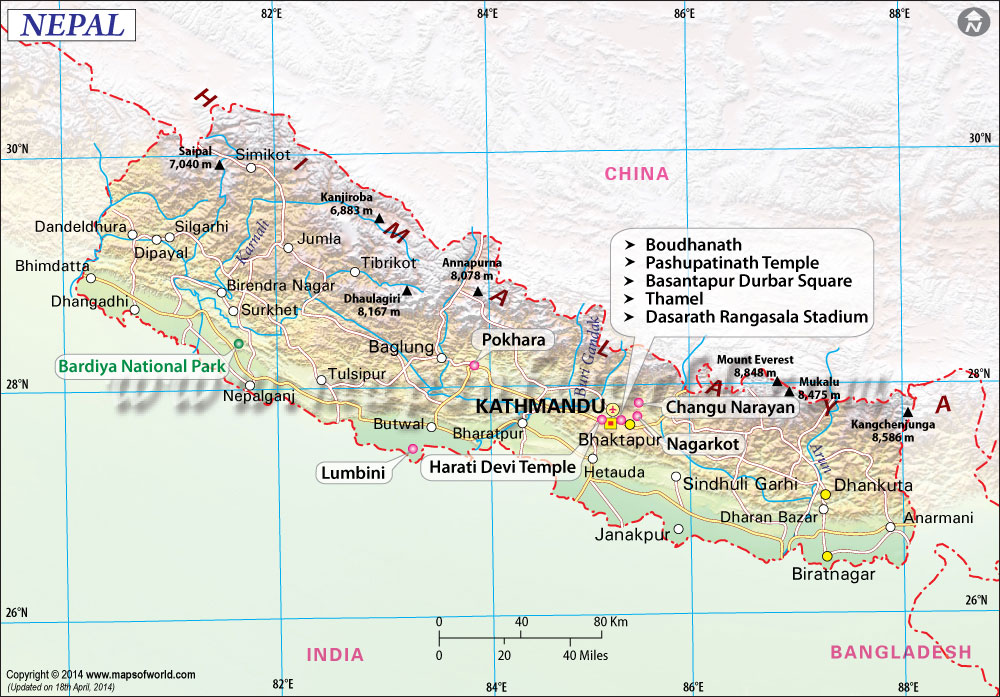
\includegraphics{./img/nepal-map.jpg}

}

\caption{\label{fig-mapa-nepal-everest}Mapa de Nepal que muestra la
ubicación del Monte Everest en el sistema de coordenadas geográficas.
Imagen de \url{https://www.mapsofworld.com/}.}

\end{figure}

Las coordenadas correspondientes a lugares y direcciones pueden
obtenerse a través de un proceso denominado
\href{https://es.wikipedia.org/wiki/Georreferenciaci\%C3\%B3n}{\emph{georreferenciación}},
mediante el cual, en general, se determina la posición espacial de
alguna entidad en un sistema de coordenadas. La georreferenciación puede
emplearse también para obtener las coordenadas de, por ejemplo,
fotografías aéreas o mapas antiguos. Es un proceso que puede resultar
complejo y costoso y para el que se han desarrollado metodologías y
plataformas especializadas (ej.
\href{https://doi.org/10.15468/doc-gg7h-s853}{Chapman AD \& Wieczorek JR
(2020) Georeferencing Best Practices},
\href{https://www.geo-locate.org/}{GEOLocate},
\href{https://nominatim.openstreetmap.org/ui/search.html}{Nominatim}).

En la actualidad, hay una gran cantidad de fuentes que generan datos
georreferenciados (i.e.~ubicados en un sistema de coordenadas). Entre
estas pueden mencionarse las tecnologías de
\href{https://ec.europa.eu/jrc/en/research-topic/earth-observation}{observación
de la Tierra (\emph{Earth Observation})} (ej.
\href{https://es.wikipedia.org/wiki/Imagen_satelital}{imágenes
satelitales}), los dispositivos móviles y los sensores remotos, entre
muchas otras.

Seguidamente, se describen dos enfoques tecnológicos para el
procesamiento de datos geoespaciales: el de los sistemas de información
geográfica y el de ciencia de datos geoespaciales.

\hypertarget{sistemas-de-informaciuxf3n-geogruxe1fica}{%
\section{Sistemas de información
geográfica}\label{sistemas-de-informaciuxf3n-geogruxe1fica}}

A principios de la década de 1960, el geógrafo inglés
\href{https://es.wikipedia.org/wiki/Roger_Tomlinson}{Roger Tomlinson}
desarrolló en Canadá el que se considera el primer sistema de
información geográfica. Se trataba del
\href{https://en.wikipedia.org/wiki/Canada_Geographic_Information_System}{Canada
Geographic Information System (CGIS)} y su objetivo fue manejar los
datos del inventario geográfico canadiense y su análisis para la gestión
del territorio rural. De manera casi simultánea al trabajo de Tomlinson,
surgieron desarrollos similares en Estados Unidos y en el Reino Unido.
El surgimiento de los sistemas de información geográfica no implicó solo
el surgimiento de nuevas herramientas de software, sino también el
desarrollo de técnicas que hasta entonces no habían sido necesarias
(Olaya 2020) como, por ejemplo, la manipulación de nuevos tipos de datos
geométricos (ej. puntos, líneas, polígonos).

En general, un sistema de información geográfica (SIG) maneja datos
georreferenciados y los asocia con datos convencionales (ej. textos,
números), como se muestra en la Figure~\ref{fig-mapa-qgis}.

\begin{figure}

{\centering 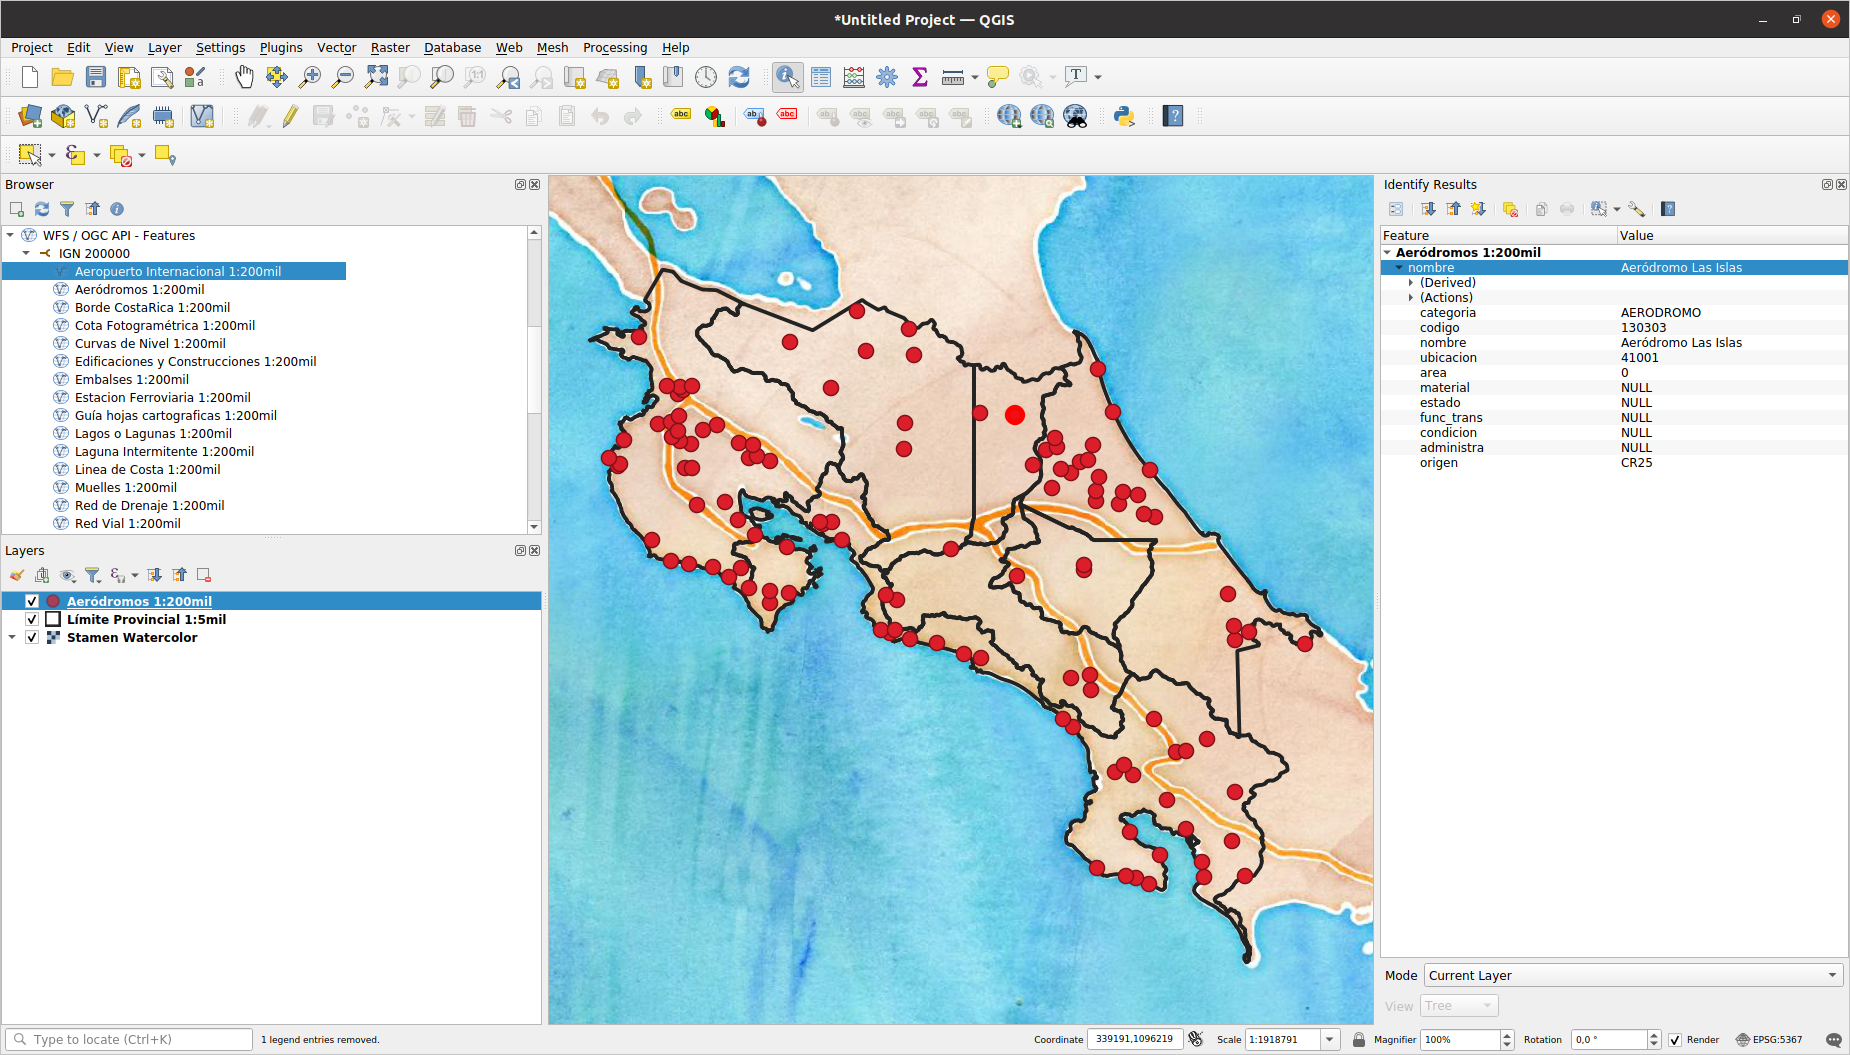
\includegraphics[width=6.17in,height=\textheight]{./img/mapa-qgis.png}

}

\caption{\label{fig-mapa-qgis}Mapa elaborado en QGIS que muestra la
ubicación de los aeródromos de Costa Rica.}

\end{figure}

Los SIG presentan los datos en capas (\emph{layers}). Por ejemplo, el
mapa de la Figure~\ref{fig-mapa-qgis} contiene una capa base raster (la
que muestra el mar y el continente), una capa de polígonos
correspondiente a las provincias de Costa Rica y una capa de puntos
correspondiente a los aeródromos. A la izquierda puede apreciarse la
lista de esas capas y a la derecha un cuadro con información detallada
sobre uno de los aeródromos.

Los SIG de escritorio (ej.
\href{https://www.esri.com/en-us/arcgis/products/arcgis-desktop/overview}{ArcGIS
Desktop}, \href{https://www.qgis.org/}{QGIS}) son herramientas con
interfaces de usuario muy gráficas e intuitivas, que no requieren de
conocimientos de programación de computadoras y que permiten generar
cartografía de alta calidad. Sin embargo, son poco flexibles y los
resultados que producen son difícilmente
\href{https://es.wikipedia.org/wiki/Reproducibilidad_y_repetibilidad}{reproducibles}.

\hypertarget{ciencia-de-datos-geoespaciales}{%
\section{Ciencia de datos
geoespaciales}\label{ciencia-de-datos-geoespaciales}}

Durante la última década, el uso de SIG se ha complementado con el de
\href{https://es.wikipedia.org/wiki/Ciencia_de_datos}{ciencia de datos},
lo que posibilitado enriquecer la visualización y el análisis de datos
geoespaciales mediante lenguajes de programación como
\href{https://www.python.org/}{Python},
\href{https://www.r-project.org/}{R} o
\href{http://www.ecma-international.org/publications-and-standards/standards/ecma-262/}{JavaScript},
entre otros.

El uso de técnicas de ciencia de datos y de otros campos relacionados
(ej.
\href{https://es.wikipedia.org/wiki/Aprendizaje_autom\%C3\%A1tico}{aprendizaje
automatizado}, \href{https://es.wikipedia.org/wiki/Macrodatos}{\emph{big
data}}) ha permitido aplicar a los datos geoespaciales técnicas y
metodologías como
\href{https://es.wikipedia.org/wiki/An\%C3\%A1lisis_de_la_regresi\%C3\%B3n}{análisis
de regresión} y
\href{https://es.wikipedia.org/wiki/Clasificaci\%C3\%B3n_estad\%C3\%ADstica}{clasificación
estadística}.

\hypertarget{reproducibilidad}{%
\section{Reproducibilidad}\label{reproducibilidad}}

Una de las principales características que distingue al enfoque de
ciencia de datos del enfoque de SIG es la
\href{https://es.wikipedia.org/wiki/Reproducibilidad_y_repetibilidad}{reproducibilidad}.
En general, la reproducibilidad es la capacidad de un ensayo o
experimento de ser reproducido por otros. Más formalmente, en
investigación cuantitativa, un análisis se considera reproducible si
\emph{``el código fuente y los datos utilizados por un investigador para
llegar a un resultado están disponibles y son suficientes para que otro
investigador, trabajando de manera independiente, pueda llegar al mismo
resultado''} (Gandrud 2020).

La reproducibilidad, junto con la
\href{https://es.wikipedia.org/wiki/Falsabilidad}{falsabilidad}, es uno
de los pilares del
\href{https://es.wikipedia.org/wiki/M\%C3\%A9todo_cient\%C3\%ADfico}{método
científico}. Sin embargo, en años recientes, se ha generado una
creciente preocupación debido a que muchos estudios científicos
publicados fallan las pruebas de reproducibilidad (véase, por ejemplo,
\href{https://www.nytimes.com/2013/04/19/opinion/krugman-the-excel-depression.html}{\emph{The
Excel Depression}, de Paul Krugman}), dando lugar a una
\href{https://es.wikipedia.org/wiki/Crisis_de_replicaci\%C3\%B3n}{crisis
de reproducibilidad o replicabilidad} en varias ciencias.

El concepto de reproducibilidad es cada vez más importante debido, entre
otras razones, al aumento exponencial de datos disponibles y a la
aplicación de la programación de computadoras, para procesar estos
datos, por parte de especialistas de muchas disciplinas.

Alex Singleton y otros autores (Singleton, Spielman, and Brunsdon 2016)
han identificado los siguientes retos para la reproducibilidad en
ciencia de datos geoespaciales:

\begin{enumerate}
\def\labelenumi{\arabic{enumi}.}
\tightlist
\item
  Los datos deben ser de dominio público y estar disponibles para los
  investigadores.
\item
  El software utilizado debe ser de código abierto (\emph{open source})
  y estar disponible para ser revisado.
\item
  Siempre que sea posible, los
  \href{https://es.wikipedia.org/wiki/Flujo_de_trabajo}{flujos de
  trabajo} deben ser públicos y con enlaces a los datos, software y
  métodos de análisis, junto con la documentación necesaria.
\item
  El proceso de
  \href{https://es.wikipedia.org/wiki/Revisi\%C3\%B3n_por_pares}{revisión
  por pares (\emph{peer review process})} y la publicación académica
  deben requerir la presentación de un modelo de flujo de trabajo e
  idealmente la disponibilidad de los materiales necesarios para la
  replicación.
\item
  En los casos en los que la reproducibilidad total no sea posible (ej.
  datos sensibles), los investigadores deben esforzarse por incluir
  todos los aspectos que puedan de un marco de trabajo abierto.
\end{enumerate}

En general, el estándar mínimo de reproducibilidad requiere que los
datos y el código fuente estén disponibles para otros investigadores
(Peng 2011). Sin embargo, dependiendo de las circunstancias y recursos
disponibles, existe todo un espectro de posibilidades, que se ilustra en
la Figure~\ref{fig-espectro-reproducibilidad}.

\begin{figure}

{\centering 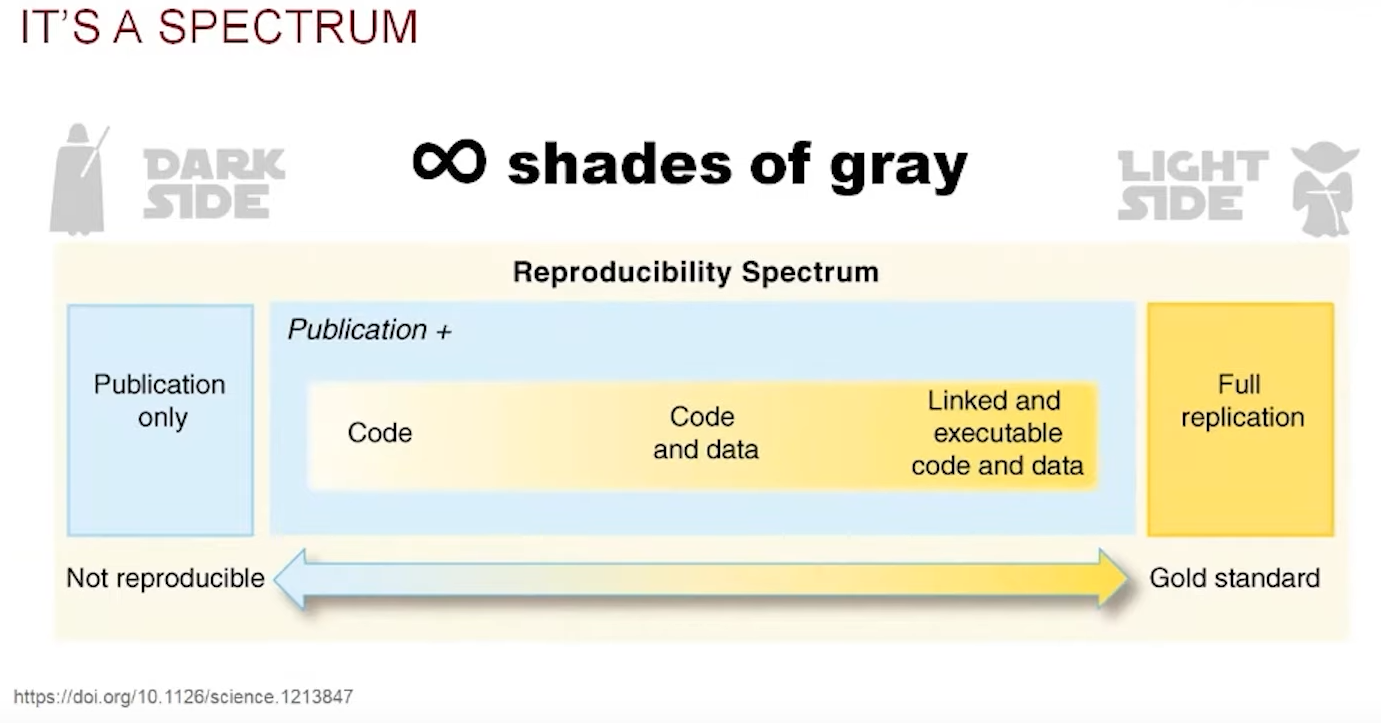
\includegraphics[width=4.6in,height=\textheight]{./img/espectro-reproducibilidad.png}

}

\caption{\label{fig-espectro-reproducibilidad}Espectro de
reproducibilidad. Imagen de
\href{https://www.youtube.com/watch?v=ZjXb53pOor0}{Anita Graser}, con
base en \href{https://doi.org/10.1126/science.1213847}{(Peng, 2001)}.}

\end{figure}

\hypertarget{herramientas-para-facilitar-la-reproducibilidad}{%
\subsection{Herramientas para facilitar la
reproducibilidad}\label{herramientas-para-facilitar-la-reproducibilidad}}

En esta sección se destacan dos tipos de herramientas que en la
actualidad se consideran esenciales para apoyar la reproducibilidad de
una investigación: los lenguajes de marcado y los sistemas de control de
versiones.

La documentación es vital durante todo el ciclo de vida de una
investigación reproducible. Para documentar, se recomienda utilizar
mecanismos estandarizados y abiertos como el
\href{https://es.wikipedia.org/wiki/HTML}{lenguaje de marcado de
hipertexto (HTML, en inglés, \emph{HyperText Markup Language})} o
\href{https://en.wikipedia.org/wiki/Markdown}{Markdown}, con los cuales
pueden crearse documentos mediante editores de texto simples (i.e.~no se
requiere de software propietario), y exportables a varios formatos (ej.
\href{https://es.wikipedia.org/wiki/LaTeX}{LaTeX},
\href{https://es.wikipedia.org/wiki/PDF}{PDF}).

Para dar mantenimiento, tanto al código fuente como a la documentación,
es necesario un sistema de
\href{https://es.wikipedia.org/wiki/Control_de_versiones}{control de
versiones} como \href{https://es.wikipedia.org/wiki/Git}{Git}, el cual
permite llevar el registro de los cambios en archivos y también facilita
el trabajo colaborativo al reunir las modificaciones hechas por varias
personas. Git es usado en varias plataformas que comparten código fuente
(ej. \href{https://github.com/}{GitHub},
\href{https://about.gitlab.com/}{GitLab}) y que ofrecen servicios
relacionados, como hospedaje de sitios web.

\hypertarget{markdown---lenguaje-de-marcado}{%
\chapter{Markdown - lenguaje de
marcado}\label{markdown---lenguaje-de-marcado}}

\hypertarget{trabajo-previo-1}{%
\section{Trabajo previo}\label{trabajo-previo-1}}

\hypertarget{tutoriales}{%
\subsection{Tutoriales}\label{tutoriales}}

\emph{Markdown Tutorial}. (s. f.). Recuperado 19 de marzo de 2022, de
\url{https://www.markdowntutorial.com/}

\hypertarget{otros}{%
\subsection{Otros}\label{otros}}

\begin{itemize}
\tightlist
\item
  Instale en su computadora el
  \href{https://cloud.r-project.org/}{sistema base del lenguaje R} y
  luego el ambiente integrado de desarrollo
  \href{https://www.rstudio.com/products/rstudio/download/\#download}{RStudio
  Desktop}.
\item
  Cree una cuenta gratuita en la plataforma de desarrollo colaborativo
  \href{https://github.com/}{GitHub}.
\end{itemize}

\hypertarget{resumen}{%
\section{Resumen}\label{resumen}}

Markdown es un lenguaje de marcado ligero ampliamente utilizado en
comunicación científica, documentación de programas e investigación
reproducible.

\hypertarget{descripciuxf3n-general}{%
\section{Descripción general}\label{descripciuxf3n-general}}

\href{https://daringfireball.net/projects/markdown/}{Markdown} es un
\href{https://es.wikipedia.org/wiki/Lenguaje_de_marcado}{lenguaje de
marcado} creado en 2004 por John Gruber. Las ``marcas'' se utilizan para
brindar información acerca de la presentación (ej. negritas, itálicas) o
la estructura (ej. títulos, encabezados) de un documento. Se caracteriza
por ser más sencillo de leer y de usar que otros lenguajes de marcado
(ej. \href{https://es.wikipedia.org/wiki/HTML}{Lenguaje de marcado de
Hipertexto o HTML}), por lo que se considera un
\href{https://es.wikipedia.org/wiki/Lenguaje_de_marcas_ligero}{lenguaje
de marcado ligero}. Los documentos escritos en Markdown pueden
exportarse a una gran variedad de formatos (ej. HTML, DOC, PDF, LaTex)
para ser usados en libros, presentaciones o páginas web, entre otros.
Markdown es ampliamente utilizado en comunicación científica,
documentación de programas e investigación reproducible.

\hypertarget{variaciones}{%
\section{Variaciones}\label{variaciones}}

Las variaciones de Markdown, también llamadas \emph{flavors}, son
extensiones o modificaciones de la especificación original. Entre las
más populares están:

\begin{itemize}
\tightlist
\item
  \href{https://rmarkdown.rstudio.com/}{R Markdown}: para el lenguaje R.
\item
  \href{https://help.github.com/en/github/writing-on-github}{GitHub
  Flavored Markdown}: para la plataforma GitHub.
\item
  \href{https://github.com/Python-Markdown/markdown}{Python Markdown}:
  para el lenguaje Python.
\item
  \href{https://pandoc.org/MANUAL.html\#pandocs-markdown}{Pandoc's
  Markdown}: para el programa \href{https://pandoc.org/}{Pandoc} de
  conversión entre formatos.
\item
  \href{https://kramdown.gettalong.org/quickref.html}{Kramdown}: para el
  lenguaje Ruby.
\end{itemize}

Puede verse una lista más extensa en
\url{https://github.com/commonmark/commonmark-spec/wiki/markdown-flavors}.

\hypertarget{sintaxis}{%
\section{Sintaxis}\label{sintaxis}}

La sintaxis de Markdown permite especificar diferentes componentes de un
documento, entre los que están:

\begin{itemize}
\tightlist
\item
  Encabezados.
\item
  Estilos (ej. negritas, itálicas).
\item
  Citas textuales.
\item
  Enlaces a otros documentos (ej. páginas web).
\item
  Imágenes.
\item
  Listas.
\end{itemize}

\hypertarget{encabezados}{%
\subsection{Encabezados}\label{encabezados}}

Pueden definirse seis niveles de encabezados, mediante símbolos de
numeral (\texttt{\#}) antes del texto. El primer nivel es el de tamaño
de texto más grande y el sexto el más pequeño. En la parte izquierda de
la Figure~\ref{fig-md-encabezados} se muestra la sintaxis Markdown de
los encabezados y a la derecha la forma en que se despliegan en un
documento.

\begin{figure}

{\centering 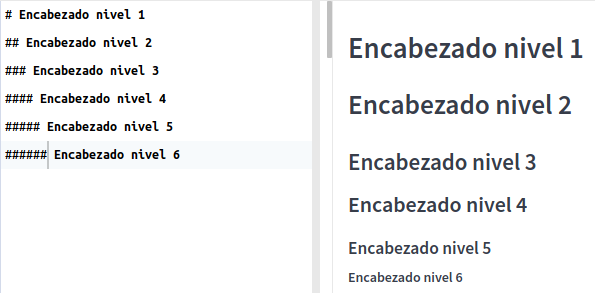
\includegraphics[width=1.98in,height=\textheight]{./img/md-encabezados.png}

}

\caption{\label{fig-md-encabezados}Sintaxis de Markdown - encabezados.}

\end{figure}

\hypertarget{ituxe1licas}{%
\subsection{Itálicas}\label{ituxe1licas}}

Se definen con un asterisco (\texttt{*}) antes y después del texto o con
un guión bajo (\texttt{\_}) antes y después del texto.

\begin{figure}

{\centering 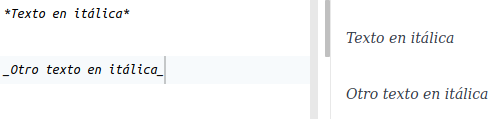
\includegraphics[width=1.66in,height=\textheight]{./img/md-italica.png}

}

\caption{\label{fig-md-italicas}Sintaxis de Markdown - itálicas.}

\end{figure}

\hypertarget{negritas}{%
\subsection{Negritas}\label{negritas}}

Se definen con dos asteriscos (\texttt{**}) antes y después del texto o
con dos guiones bajos (\texttt{\_\_}) antes y después del texto.

\begin{figure}

{\centering 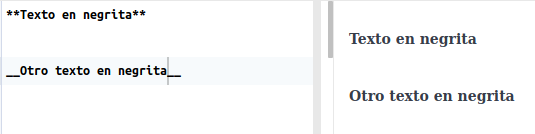
\includegraphics[width=1.78in,height=\textheight]{./img/md-negrita.png}

}

\caption{\label{fig-md-negritas}Sintaxis de Markdown - negritas.}

\end{figure}

\hypertarget{citas-textuales}{%
\subsection{Citas textuales}\label{citas-textuales}}

Se definen con un símbolo de ``mayor que'' (\texttt{\textgreater{}})
antes de cada línea.

\begin{figure}

{\centering 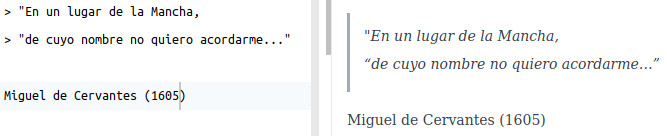
\includegraphics[width=2.22in,height=\textheight]{./img/md-cita.png}

}

\caption{\label{fig-md-citas}Sintaxis de Markdown - citas textuales.}

\end{figure}

\hypertarget{enlaces-hipervuxednculos}{%
\subsection{Enlaces (hipervínculos)}\label{enlaces-hipervuxednculos}}

Se definen con paréntesis cuadrados (\texttt{{[}{]}}) seguidos de
paréntesis redondos (\texttt{()}). En los paréntesis cuadrados se coloca
(opcionalmente) el texto del enlace y en los redondos la dirección del
documento.

\begin{figure}

{\centering 
\includegraphics[width=2.08in,height=\textheight]{./img/md-enlace.png}

}

\caption{\label{fig-md-enlaces}Sintaxis de Markdown - enlaces.}

\end{figure}

\hypertarget{imuxe1genes}{%
\subsection{Imágenes}\label{imuxe1genes}}

Se definen con un signo de admiración de cierre (\texttt{!}), paréntesis
cuadrados (\texttt{{[}{]}}) y paréntesis redondos (\texttt{()}). En los
paréntesis cuadrados se coloca (opcionalmente) un texto alternativo de
la imagen y en los redondos la dirección de la imagen, ya sea local o
remota.

\begin{figure}

{\centering 
\includegraphics[width=4.03in,height=\textheight]{./img/md-imagen.png}

}

\caption{\label{fig-md-imagenes}Sintaxis de Markdown - imágenes.}

\end{figure}

\hypertarget{listas-numeradas}{%
\subsection{Listas numeradas}\label{listas-numeradas}}

Se definen con números (\texttt{1.\ 2.\ 3.\ ...}) antes de cada
elemento.

\begin{figure}

{\centering 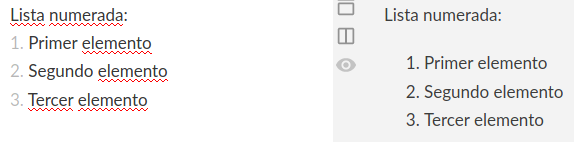
\includegraphics[width=1.91in,height=\textheight]{./img/md-lista-numerada.png}

}

\caption{\label{fig-md-listas-numeradas}Sintaxis de Markdown - listas
numeradas.}

\end{figure}

\hypertarget{listas-no-numeradas}{%
\subsection{Listas no numeradas}\label{listas-no-numeradas}}

Se definen con guiones (\texttt{-}) o asteriscos (\texttt{*}) antes de
cada elemento.

\begin{figure}

{\centering 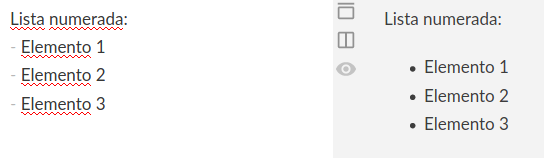
\includegraphics[width=1.81in,height=\textheight]{./img/md-lista-no-numerada.png}

}

\caption{\label{fig-md-listas-no-numeradas}Sintaxis de Markdown - listas
no numeradas.}

\end{figure}

\hypertarget{otros-elementos-de-sintaxis}{%
\subsection{Otros elementos de
sintaxis}\label{otros-elementos-de-sintaxis}}

Para conocer otros elementos de la sintaxis de Markdown, se recomienda
revisar en detalle la \href{https://www.markdownguide.org/}{Guía de
referencia de Markdown}.

\hypertarget{ejercicios}{%
\section{Ejercicios}\label{ejercicios}}

\begin{enumerate}
\def\labelenumi{\arabic{enumi}.}
\tightlist
\item
  Cree un documento Markdown llamado \texttt{README.md}, en RStudio, y
  escriba en este un breve perfil académico (\emph{curriculum}
  académico).

  \begin{itemize}
  \tightlist
  \item
    Incluya información como: nombre, fotografía, datos de contacto,
    áreas de interés, carrera, cursos aprobados, publicaciones, etc.
  \item
    Puede usar información ficticia (\textbf{no incluya datos
    confidenciales o sensibles}).
  \item
    Especifique la fuente de las imágenes (y de cualquier otra
    información para la que sea necesario) y no utilice imágenes para
    las que no tiene autorización. Considere utilizar sitios con
    imágenes con licencias abiertas (ej.
    \href{https://commons.wikimedia.org/}{Wikimedia Commons},
    \href{https://unsplash.com/}{Unsplash},
    \href{https://www.freeimages.com/}{FreeImages}).
  \item
    Asegúrese de utilizar los siguientes elementos de sintaxis Markdown:

    \begin{itemize}
    \tightlist
    \item
      Varios niveles de encabezados.
    \item
      Negritas e itálicas.
    \item
      Listas.
    \item
      Enlaces a sitios web.
    \item
      Imágenes (al menos una local y una remota).
    \end{itemize}
  \end{itemize}
\item
  Cree un repositorio en \href{https://github.com/}{GitHub} llamado
  \texttt{perfil-academico} y suba a este el documento que creó en el
  paso 1.
\item
  Cree un sitio web en \href{https://pages.github.com/}{GitHub Pages}
  con el repositorio creado en el paso 2.
\end{enumerate}

\hypertarget{recursos-de-interuxe9s}{%
\section{Recursos de interés}\label{recursos-de-interuxe9s}}

Carrera Arias, F. J. (2020). \emph{How to Install R on Windows, Mac OS
X, and Ubuntu Tutorial}. DataCamp Community.
\url{https://www.datacamp.com/community/tutorials/installing-R-windows-mac-ubuntu}

\emph{Markdown Guide}. (s. f.). Recuperado 10 de abril de 2022, de
\url{https://www.markdownguide.org/}

\hypertarget{git---sistema-de-control-de-versiones}{%
\chapter{Git - sistema de control de
versiones}\label{git---sistema-de-control-de-versiones}}

\hypertarget{trabajo-previo-2}{%
\section{Trabajo previo}\label{trabajo-previo-2}}

\hypertarget{tutoriales-1}{%
\subsection{Tutoriales}\label{tutoriales-1}}

Abba, I. V. (2021). \emph{Git and GitHub Tutorial -- Version Control for
Beginners}. FreeCodeCamp.Org.
\url{https://www.freecodecamp.org/news/git-and-github-for-beginners/}

\hypertarget{otros-1}{%
\subsection{Otros}\label{otros-1}}

Instale en su computadora el sistema de control de versiones
\href{https://git-scm.com/downloads}{Git}.

\hypertarget{resumen-1}{%
\section{Resumen}\label{resumen-1}}

Git es un sistema para administrar versiones de código fuente o, en
general, de cualquier conjunto de archivos.

\hypertarget{descripciuxf3n-general-1}{%
\section{Descripción general}\label{descripciuxf3n-general-1}}

\href{https://git-scm.com/}{Git} es un sistema de
\href{https://es.wikipedia.org/wiki/Control_de_versiones}{control de
versiones} diseñado para ``rastrear'' cambios en el código fuente
durante el proceso de desarrollo de software. Sin embargo, puede ser
utilizado para llevar el control de los cambios en cualquier conjunto de
archivos (ej.
\href{https://guides.github.com/features/wikis/}{documentación},
\href{https://techcrunch.com/2013/10/09/splice-music/}{música}).

Un sistema de control de versiones proporciona, entre otras ventajas:

\begin{itemize}
\tightlist
\item
  La capacidad de recuperar versiones anteriores de los archivos.
\item
  La capacidad de integrar modificaciones efectuadas por varias personas
  en el mismo conjunto de archivos.
\item
  La capacidad de mantener varias ``ramas'' (\emph{branches}) de un
  producto (ej. ``estable'', ``evaluación'', ``inestable'', como en el
  caso de \href{https://www.debian.org/releases/}{Debian Linux},
  \href{https://grass.osgeo.org/download/software/sources/}{GRASS GIS} y
  muchos otros proyectos de software libre).
\item
  Facilidades para mantener redundancia y respaldos de los archivos (ej.
  \href{https://archiveprogram.github.com/}{Programa de respaldos de
  GitHub}). Esta es una facilidad que implementan algunos servicios en
  la nube.
\end{itemize}

Git fue diseñado por Linus Torvalds en 2005 durante del desarrollo del
\emph{kernel} del sistema operativo Linux. Se caracteriza por ser un
\href{https://es.wikipedia.org/wiki/Control_de_versiones_distribuido}{sistema
de control de versiones distribuido}, lo que significa que el código
fuente puede estar alojado en la estación de trabajo de cualquier
miembro del equipo de desarrollo. No se requiere de un repositorio
``central'', pero también se puede trabajar de esa forma.

El protocolo de Git es utilizado en varios sitios que proveen servicios
de alojamiento de software, entre los que están
\href{https://sourceforge.net/}{SourceForge},
\href{https://bitbucket.org/}{Bitbucket},
\href{https://about.gitlab.com/}{GitLab} y
\href{https://github.com/}{GitHub}.

\hypertarget{funcionamiento-de-git}{%
\section{Funcionamiento de Git}\label{funcionamiento-de-git}}

Desde el punto de vista de un usuario de Git (ej. un programador), Git
se utiliza para sincronizar la versión local (i.e.~en una computadora
personal) de un conjunto de archivos, llamado proyecto o repositorio,
con la versión que está alojada en un sistema remoto (ej. GitHub). Cada
repositorio se almacena en un directorio (carpeta) del sistema
operativo. La sincronización se realiza principalmente a través de dos
operaciones:

\begin{itemize}
\tightlist
\item
  \textbf{\emph{push}}: para ``subir'' al repositorio remoto los cambios
  realizados en el repositorio local. Esta operación se realiza mediante
  el comando \href{https://git-scm.com/docs/git-push}{git push}. Es
  probable que el sistema remoto le solicite al usuario algún tipo de
  autenticación (ej. nombre de usuario y clave).
\item
  \textbf{\emph{pull}}: para ``bajar'' al repositorio local los cambios
  realizados en el repositorio remoto. Esta operación se realiza
  mediante el comando \href{https://git-scm.com/docs/git-pull}{git
  pull}.
\end{itemize}

Las operaciones \emph{push} y \emph{pull} se ilustran en la
Figure~\ref{fig-git-push-pull}.

\begin{figure}

{\centering 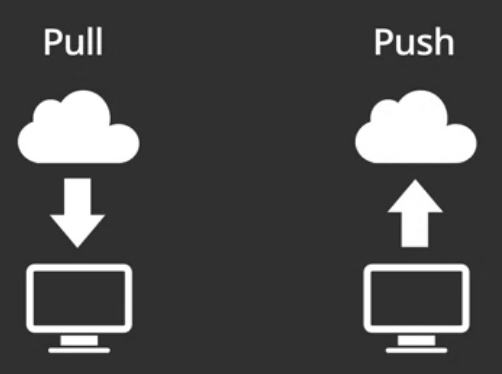
\includegraphics[width=1.67in,height=\textheight]{./img/git-push-pull.png}

}

\caption{\label{fig-git-push-pull}Operaciones \emph{push} y \emph{pull}.
Imagen de
\href{https://www.coursera.org/learn/reproducible-templates-analysis/lecture/NGbQv/git-and-github-part-1}{Melinda
Higgins}.}

\end{figure}

Antes de un \emph{push}, el usuario debe seleccionar los archivos que
desea subir mediante el comando
\href{https://git-scm.com/docs/git-add}{git add}, el cual pasa los
archivos a un ``área de espera'' (\emph{staging area}). Luego debe
usarse el comando \href{https://git-scm.com/docs/git-commit}{git commit}
para ``guardar'' los cambios pendientes en el área de espera. Cada
\emph{commit} guarda el estado del conjunto de archivos en un momento
específico (\emph{snapshot}).

La relación entre estas operaciones de Git, se ilustra en la
Figure~\ref{fig-git-push-pull-commit}.

\begin{figure}

{\centering 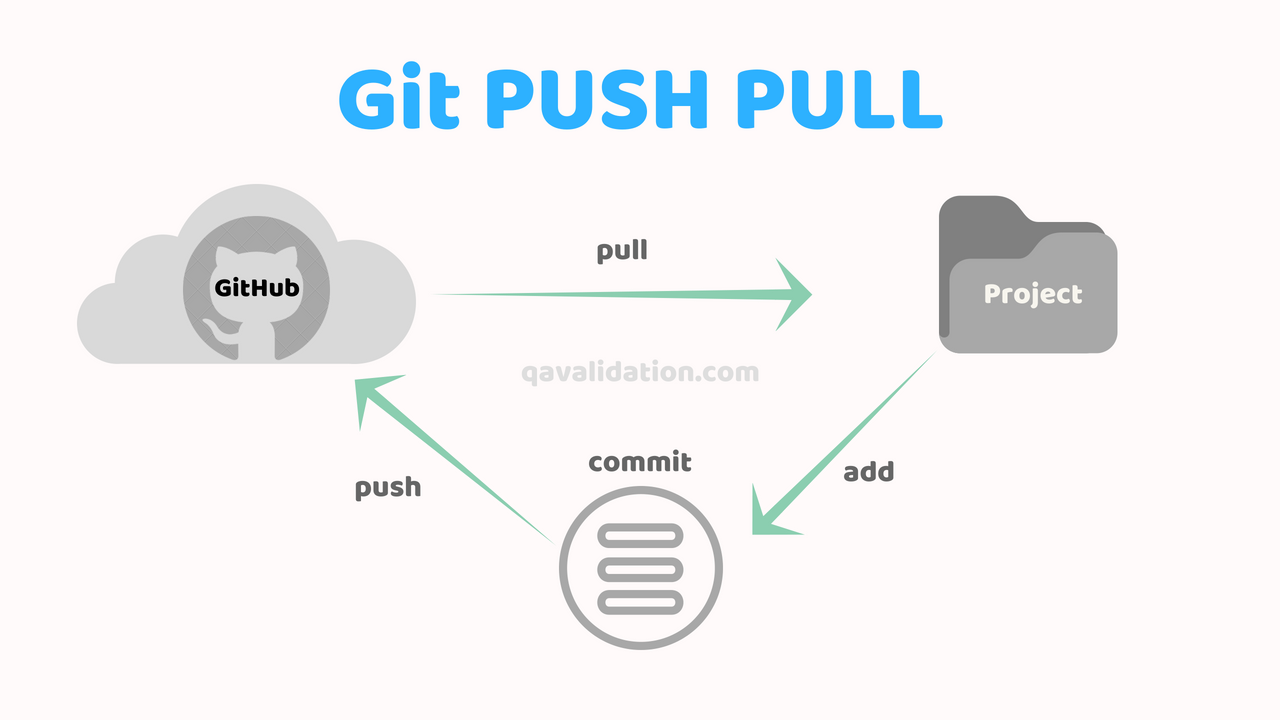
\includegraphics[width=4.27in,height=\textheight]{./img/git-push-pull-commit.png}

}

\caption{\label{fig-git-push-pull-commit}Operaciones de Git. Imagen de
\href{https://medium.com/@stevenklavins94/version-control-part-4-c9387cf5b33e}{Steven
Klavins}.}

\end{figure}

En la Figure~\ref{fig-git-stage-commit-push}, se muestra el
funcionamiento de Git mediante una comparación con el procesamiento de
una compra en línea.

\begin{figure}

{\centering 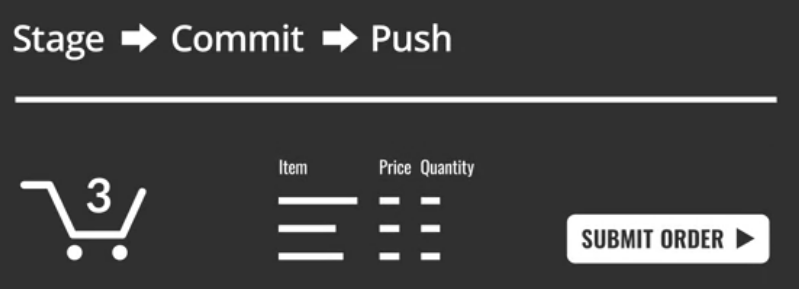
\includegraphics[width=2.66in,height=\textheight]{./img/git-stage-commit-push.png}

}

\caption{\label{fig-git-stage-commit-push}Operaciones de Git y compras
en línea. Imagen de
\href{https://www.coursera.org/learn/reproducible-templates-analysis/lecture/NGbQv/git-and-github-part-2}{Melinda
Higgins}.}

\end{figure}

Otras operaciones de Git de uso frecuente son:

\begin{itemize}
\tightlist
\item
  \href{https://git-scm.com/docs/git-config}{git config}: para
  especificar opciones globales de la sesión de Git (ej. nombre del
  usuario, dirección de correo electrónico).
\item
  \href{https://git-scm.com/docs/git-init}{git init}: para inicializar
  un repositorio git.
\item
  \href{https://git-scm.com/docs/git-clone}{git clone}: para clonar
  (i.e.~copiar) un repositorio remoto en la computadora local.
\item
  \href{https://git-scm.com/docs/git-status}{git status}: para revisar
  el estado de los archivos y, por ejemplo, saber cuales deben pasarse
  al área de espera.
\item
  \href{https://git-scm.com/docs/git-log}{git log}: para revisar el
  historial de \emph{commits}.
\item
  \href{https://git-scm.com/docs/git-show}{git show}: para visualizar
  los cambios efectuados en los \emph{commits}.
\item
  \href{https://git-scm.com/docs/git-reset}{git reset}: para regresar al
  estado correspondiente a un \emph{commit} anterior.
\end{itemize}

\hypertarget{ejemplos-de-uso}{%
\section{Ejemplos de uso}\label{ejemplos-de-uso}}

\hypertarget{clonaciuxf3n-de-un-repositorio-remoto-y-sincronizaciuxf3n-de-los-cambios-efectuados-localmente}{%
\subsection{Clonación de un repositorio remoto y sincronización de los
cambios efectuados
localmente}\label{clonaciuxf3n-de-un-repositorio-remoto-y-sincronizaciuxf3n-de-los-cambios-efectuados-localmente}}

Para seguir este ejemplo:

\begin{enumerate}
\def\labelenumi{\arabic{enumi}.}
\setcounter{enumi}{-1}
\tightlist
\item
  Obtenga un \emph{token} de GitHub en la siguiente opción de menú de su
  perfil de usuario: \emph{Settings - Developer settings - Personal
  access tokens}. Seleccione las operaciones de tipo ``repo''. Copie el
  \emph{token} en un lugar seguro, ya que lo necesitará para
  autenticarse en GitHub.
\item
  Realice un \emph{fork} a su cuenta en GitHub del repositorio
  localizado en la dirección
  \url{https://github.com/pf0953-programacionr/2022-ii-tutorial-git-repo-ejemplo}.
  Obtendrá un repositorio llamado
  ``https://github.com/{[}nombre-usuario{]}/2022-ii-tutorial-git-repo-ejemplo'',
  en donde {[}nombre-usuario{]} es su nombre de usuario en GitHub.
\item
  Con la opción \emph{File - New Project - Version Control - Git} de
  RStudio, clone a su computadora el repositorio que acaba de bifurcar.
\item
  Con el editor de RStudio, abra el archivo \texttt{README.md}, agregue
  una línea y guarde el archivo.
\item
  Luego, ejecute los siguientes comandos desde la la ventana
  \emph{Terminal} de RStudio. Nota: las líneas que empiezan con
  \texttt{\#} son comentarios.
\end{enumerate}

\begin{Shaded}
\begin{Highlighting}[]
\NormalTok{\# a. Parámetros de configuración: nombre y dirección de correo del usuario.}
\NormalTok{\#    Debe cambiar [email{-}usuario] y [nombre{-}usuario] por sus propios datos.}
\NormalTok{git config {-}{-}global user.email [email{-}usuario]}
\NormalTok{git config {-}{-}global user.name [nombre{-}usuario]}
\NormalTok{\# Para revisar los parámetros de configuración:}
\NormalTok{git config {-}{-}global {-}{-}list}

\NormalTok{\# b. Revisión de los archivos con modificaciones.}
\NormalTok{git status}

\NormalTok{\# c. Adición (add) de los archivos modificados al "área de espera".}
\NormalTok{\#    El punto (.) indica que se agregarán todos los archivos modificados.}
\NormalTok{git add .}

\NormalTok{\# d. Grabado (commit) del conjunto de archivos modificados,}
\NormalTok{\#    junto con un mensaje explicativo:}
\NormalTok{git commit {-}m "Agregar línea 2"}

\NormalTok{\# e. "Subida" (push) de las modificaciones al repositorio remoto.}
\NormalTok{\#    En este paso, es posible que deba utilizar su nombre de usuario/clave}
\NormalTok{\#    o su token de GitHub para autenticarse.}
\NormalTok{git push}
\end{Highlighting}
\end{Shaded}

\begin{enumerate}
\def\labelenumi{\arabic{enumi}.}
\setcounter{enumi}{4}
\tightlist
\item
  Revise los cambios aplicados en el repositorio remoto en GitHub.
\item
  Agregue más líneas al archivo del repositorio local y sincronícelo con
  el remoto, realizando nuevamente los pasos del b al e para cada
  \emph{commit}. Recuerde que los comentarios de cada \texttt{commit}
  deben reflejar los cambios que están siendo aplicados.
\end{enumerate}

\hypertarget{recursos-de-interuxe9s-1}{%
\section{Recursos de interés}\label{recursos-de-interuxe9s-1}}

\emph{Git}. (s. f.). Recuperado 28 de agosto de 2022, de
\url{https://git-scm.com/}

\emph{GitHub Archive Program}. (s. f.). GitHub Archive Program.
Recuperado 10 de abril de 2022, de
\url{https://archiveprogram.github.com/}

Higgins, M. (s. f.). \emph{Reproducible Templates for Analysis and
Dissemination}. Coursera. Recuperado 11 de abril de 2022, de
\url{https://www.coursera.org/learn/reproducible-templates-analysis}

Klavins, S. (2020). \emph{Version Control part 1}. Medium.
\url{https://stevenklavins94.medium.com/version-control-part-1-c5f1b43127f6}

\part{II - El lenguaje de programación R}

\hypertarget{pensamiento-computacional-y-arquitectura-de-computadoras}{%
\chapter{Pensamiento computacional y arquitectura de
computadoras}\label{pensamiento-computacional-y-arquitectura-de-computadoras}}

\hypertarget{trabajo-previo-3}{%
\section{Trabajo previo}\label{trabajo-previo-3}}

\hypertarget{lecturas-1}{%
\subsection{Lecturas}\label{lecturas-1}}

Wing, J. M. (2006). Computational thinking. \emph{Communications of the
ACM, 49}(3), 33-35. \url{https://doi.org/10.1145/1118178.1118215}

\hypertarget{resumen-2}{%
\section{Resumen}\label{resumen-2}}

El pensamiento computacional es un enfoque para la resolución de
problemas basado en conceptos y métodos de las ciencias de la
computación. Los principios fundamentales del pensamiento computacional
son:

\begin{itemize}
\tightlist
\item
  \textbf{Descomposición}: división de un problema en subproblemas más
  pequeños.
\item
  \textbf{Reconocimiento de patrones}: búsqueda de similitudes en los
  problemas.
\item
  \textbf{Abstracción}: identificación de la información que se necesita
  y filtrado de la que no se necesita para resolver un problema.
\item
  \textbf{Algoritmos}: descripción, paso por paso, de la solución a un
  problema.
\end{itemize}

Las computadoras modernas están construídas con base en circuitos
integrados (CI), también llamados chips o microchips. Los CI procesan
información digital (que usa valores discretos), la cual generalmente es
binaria (i.e.~de dos valores). Los CI de una computadora procesan dos
estados correspondientes a dos niveles de tensión eléctrica: alto y
bajo. Estos estados se representan con 0 y 1. Esto facilita la
aplicación de la lógica binaria y de la aritmética binaria.

Durante el período entre las guerras mundiales, Allan Turing desarrolló
la máquina de Turing, un dispositivo teórico que manipula símbolos de
una cinta de acuerdo con una tabla de reglas. La máquina de Turing
simula el funcionamiento de un algoritmo y los conceptos de entrada,
procesamiento y salida. En 1945, John von Neumann propuso un concepto
conocido como programa almacenado, en el cual los datos y los programas
se almacenan en una estructura llamada memoria, separada del hardware
que ejecuta las instrucciones. Este modelo permite que las computadoras
sean más fáciles de reprogramar y es conocido actualmente como
arquitectura de von Neumann.

El lenguaje máquina es un conjunto de instrucciones binarias
interpretables por un CPU. Las instrucciones representan acciones a ser
ejecutadas por la computadora. Cada CPU tiene su propio lenguaje
máquina. Un programa consiste de una secuencia de instrucciones en
lenguaje máquina.

Debido a que programar una computadora en lenguaje máquina es
excesivamente lento y complicado, en la década de 1950 comenzaron a
crearse lenguajes de programación que, en lugar de unos y ceros,
consisten de instrucciones formadas por palabras, usualmente en idioma
inglés. Existe una gran variedad de lenguajes de programación que han
sido creados con diversos fines: científicos, comerciales,
educacionales, etc.

\hypertarget{diapositivas}{%
\section{Diapositivas}\label{diapositivas}}

\href{https://pf0953-programacionr.github.io/2022-ii-pensamiento_computacional-arquitectura_computadoras/}{Pensamiento
computacional y arquitectura de computadoras}

\hypertarget{r---conceptos-buxe1sicos}{%
\chapter{R - conceptos básicos}\label{r---conceptos-buxe1sicos}}

\hypertarget{trabajo-previo-4}{%
\section{Trabajo previo}\label{trabajo-previo-4}}

\hypertarget{lecturas-2}{%
\subsection{Lecturas}\label{lecturas-2}}

Grolemund, G., \& Wickham, H. (2014). \emph{Hands-On Programming with R:
Write Your Own Functions And Simulations} (capítulos 1 - 12). O'Reilly
Media. \url{https://rstudio-education.github.io/hopr/}

\hypertarget{resumen-3}{%
\section{Resumen}\label{resumen-3}}

En esta lección, se estudiarán los conceptos básicos del lenguaje de
programación R, incluyendo:

\begin{itemize}
\tightlist
\item
  Características generales de R.
\item
  El ambiente de desarrollo RStudio.
\item
  Funciones y paquetes.
\item
  Tipos de datos.
\item
  Definición de funciones.
\item
  Condicionales.
\item
  Ciclos.
\end{itemize}

\hypertarget{caracteruxedsticas-generales}{%
\section{Características generales}\label{caracteruxedsticas-generales}}

\href{https://www.r-project.org/}{R} es un lenguaje de programación
enfocado en análisis estadístico. Es ampliamente utilizado en diversas
áreas de investigación, entre las que pueden mencionarse
\href{https://en.wikipedia.org/wiki/Machine_learning}{aprendizaje
automático (\emph{machine learning})},
\href{https://en.wikipedia.org/wiki/Data_science}{ciencia de datos
(\emph{data science})} y
\href{https://en.wikipedia.org/wiki/Big_data}{\emph{big data}}, con
aplicaciones en campos como biomedicina, bioinformática y finanzas,
entre muchos otros. Fue creado por Ross Ihaka y Robert Gentleman en la
Universidad de Auckland, Nueva Zelanda, en 1993.

Algunas de las principales características de este lenguaje son:

\begin{itemize}
\tightlist
\item
  Es
  \href{https://en.wikipedia.org/wiki/Interpreter_(computing)}{interpretado}:
  las instrucciones se traducen una por una a
  \href{https://en.wikipedia.org/wiki/Machine_code}{lenguaje máquina}, a
  diferencia de los
  \href{https://en.wikipedia.org/wiki/Compiler}{lenguajes compilados},
  que traducen de manera conjunta las instrucciones de una unidad
  completa (ej. un programa o una biblioteca). Los lenguajes
  interpretados tienden a ser más lentos que los compilados, pero
  también son más flexibles.
\item
  Es
  \href{https://en.wikipedia.org/wiki/Cross-platform_software}{multiplataforma}:
  puede ejecutarse en los sistemas operativos más populares (ej.
  Microsoft Windows, macOS, Linux).
\item
  Tiene un
  \href{https://pythonconquerstheuniverse.wordpress.com/2009/10/03/static-vs-dynamic-typing-of-programming-languages/}{sistema
  de tipos de datos dinámico}: las variables pueden tomar diferentes
  tipos de datos (ej. textuales, numéricos) durante la ejecución del
  programa, a diferencia del caso de un sistema de tipos de datos
  estático, en el que las variables solo pueden tener un tipo de datos.
\item
  Soporta varios
  \href{https://en.wikipedia.org/wiki/Programming_paradigm}{paradigmas
  de programación}: los paradigmas son estilos o enfoques teóricos de
  programación. R soporta los paradigmas de
  \href{https://en.wikipedia.org/wiki/Functional_programming}{programación
  funcional},
  \href{https://en.wikipedia.org/wiki/Object-oriented_programming}{programación
  orientada a objetos},
  \href{https://en.wikipedia.org/wiki/Imperative_programming}{programación
  imperativa} y
  \href{https://en.wikipedia.org/wiki/Procedural_programming}{programación
  procedimental}.
\end{itemize}

R es un proyecto de
\href{https://en.wikipedia.org/wiki/Free_software}{software libre} que
se comparte mediante una licencia
\href{https://www.gnu.org/licenses/old-licenses/gpl-2.0.html}{GNU
General Public Licence (GNU GPL)}. Esta característica permite que la
funcionalidad original de R pueda ser ampliada mediante bibliotecas o
paquetes desarrollados por la comunidad de programadores.

Para programar en R, puede utilizarse una interfaz de línea de comandos,
editores de texto (ej. \href{https://code.visualstudio.com/}{Visual
Studio Code}, \href{https://www.vim.org/}{Vim}) y también ambientes de
desarrollo integrados (IDE, \emph{integrated development environment})
como \href{https://jupyter.org/}{Jupyter} o
\href{https://rstudio.com/}{RStudio}.

\hypertarget{el-ambiente-de-desarrollo-integrado-rstudio}{%
\section{El ambiente de desarrollo integrado
RStudio}\label{el-ambiente-de-desarrollo-integrado-rstudio}}

\href{https://www.rstudio.com/}{RStudio} es el IDE más popular para el
lenguaje R. Está disponible en una versión de escritorio (RStudio
Desktop) y en una versión para servidor (RStudio Server). Esta última
permite la conexión de varios usuarios a través de un navegador web.
RStudio se ofrece también como un servicio en la nube, a través de
\href{https://www.rstudio.com/products/cloud/}{RStudio Cloud}.

La Figure~\ref{fig-rstudio-interfaz} muestra la interfaz de RStudio.

\begin{figure}

{\centering 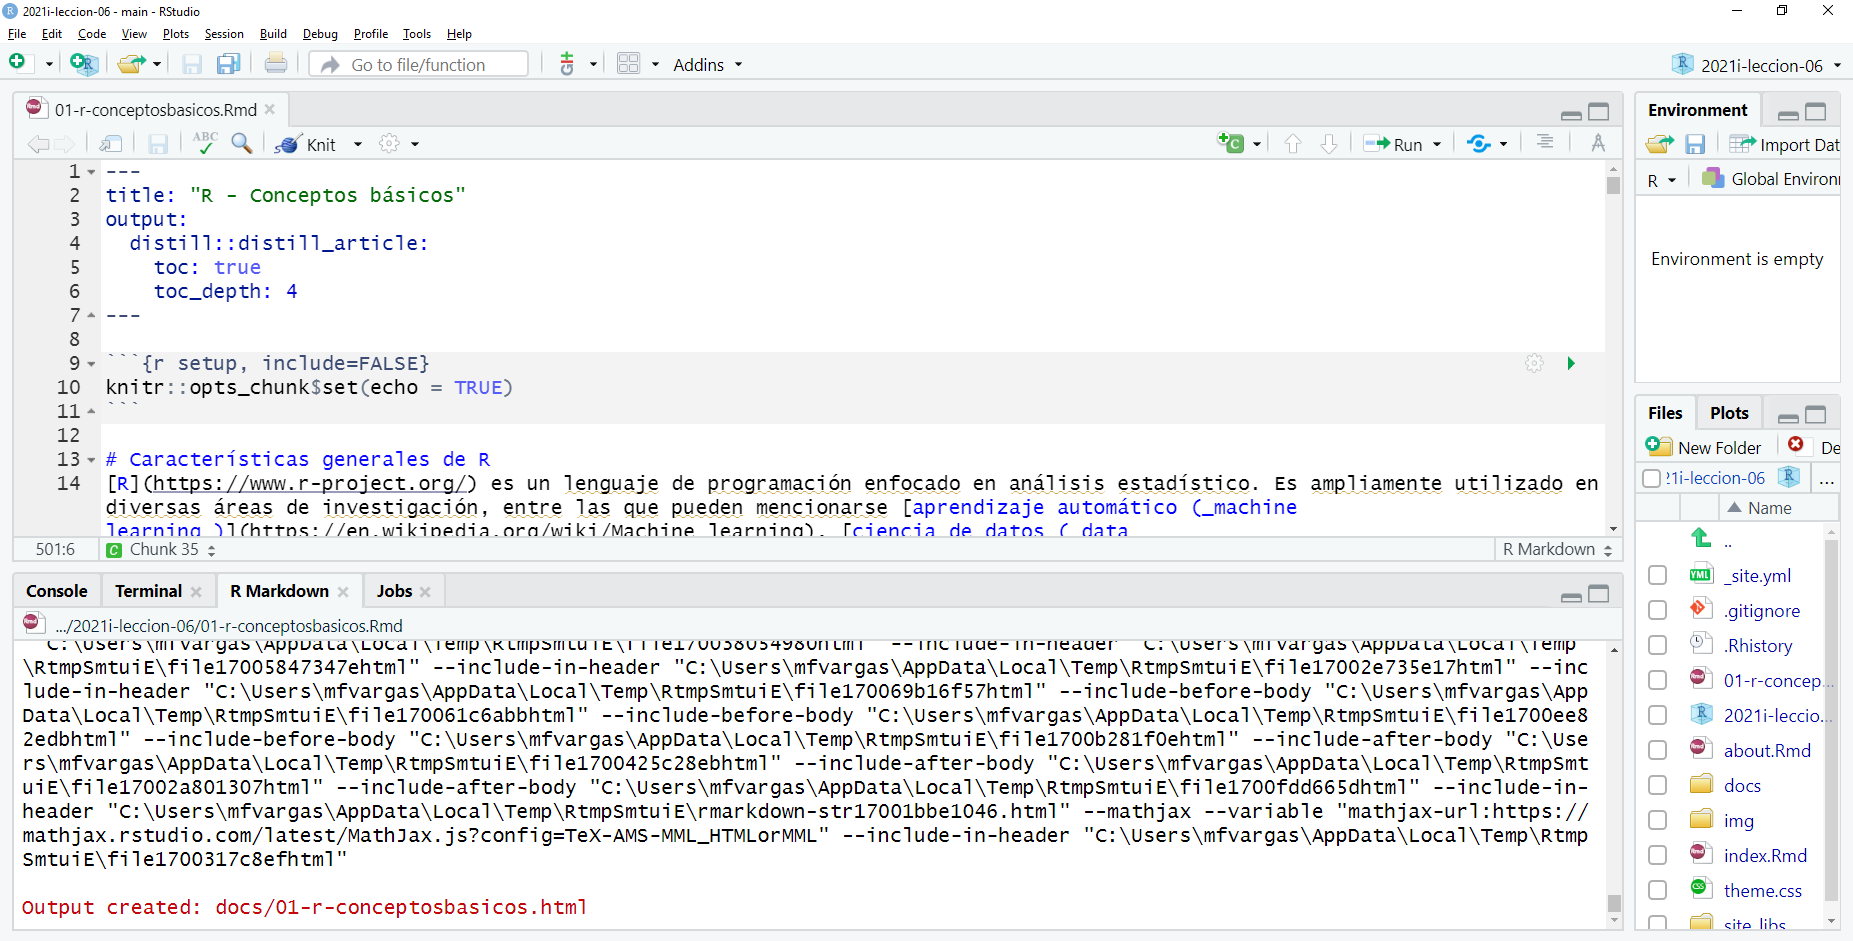
\includegraphics[width=6.18in,height=\textheight]{./img/rstudio.png}

}

\caption{\label{fig-rstudio-interfaz}Interfaz del ambiente de desarrollo
integrado RStudio.}

\end{figure}

Además de edición de código fuente en R (y otros lenguajes), RStudio
contiene capacidades para depurar código y visualizar datos en formatos
tabulares, gráficos y de mapas.

\hypertarget{conjuntos-de-datos-para-pruebas}{%
\section{Conjuntos de datos para
pruebas}\label{conjuntos-de-datos-para-pruebas}}

Para efectos de pruebas y ejemplos, la distribución base de R incorpora
varios conjuntos de datos que pueden listarse con la función
\href{https://rdrr.io/r/utils/data.html}{data()}. Para obtener
información acerca de un conjunto de datos en particular, puede
utilizarse el operador \texttt{?}.

\begin{Shaded}
\begin{Highlighting}[]
\CommentTok{\# Información sobre todos los conjuntos de datos incorporados en la distribución base de R}
\FunctionTok{data}\NormalTok{()}

\CommentTok{\# Información sobre el cojunto de datos "cars"}
\NormalTok{?cars}

\CommentTok{\# Información sobre el cojunto de datos "mtcars"}
\NormalTok{?mtcars}

\CommentTok{\# Información sobre el cojunto de datos "Iris"}
\NormalTok{?iris}
\end{Highlighting}
\end{Shaded}

Además, existen muchos sitios en Internet que brindan acceso a conjuntos
de datos que pueden utilizarse para pruebas. Por ejemplo:

\begin{itemize}
\tightlist
\item
  \href{https://www.kaggle.com/datasets}{Kaggle - conjuntos de datos}
\item
  \href{https://data.worldbank.org/indicator}{Banco Mundial -
  indicadores}
\item
  \href{https://paperswithcode.com/datasets}{Papers with Code -
  conjuntos de datos}
\end{itemize}

\hypertarget{funciones}{%
\section{Funciones}\label{funciones}}

R, al igual que otros lenguajes de programación, estructura su
funcionalidad en unidades de
\href{https://en.wikipedia.org/wiki/Source_code}{código fuente} llamadas
\href{https://cran.r-project.org/doc/manuals/r-release/R-lang.html\#Functions}{funciones}.
Cada función realiza una tarea específica como, por ejemplo, un cálculo
matemático y, por lo general, retorna un valor como salida. Todas las
funciones tienen un nombre y, opcionalmente, un conjunto de argumentos
que especifican los datos de entrada que procesa la función. Los
argumentos se escriben entre paréntesis redondos (\texttt{()}) y estos
siempre deben incluirse, aún en el caso de que la función no tenga
ningún argumento. Si la función tiene varios argumentos, deben separarse
mediante comas (\texttt{,}).

\hypertarget{ejemplos}{%
\subsection{Ejemplos}\label{ejemplos}}

La función \href{https://rdrr.io/r/base/print.html}{print()} recibe como
argumento un valor (ej. un texto o un número) para imprimirlo en la
pantalla. En el siguiente fragmento de código en R, se utiliza
\texttt{print()} para imprimir la hilera
\href{https://en.wikipedia.org/wiki/\%22Hello,_World!\%22_program}{``Hola
mundo''}. Nótese el uso del símbolo \texttt{\#} para comentarios
(i.e.~texto que no es código ejecutable).

\begin{Shaded}
\begin{Highlighting}[]
\CommentTok{\# Impresión de una hilera de caracteres}
\FunctionTok{print}\NormalTok{(}\StringTok{"Hola mundo"}\NormalTok{)}
\end{Highlighting}
\end{Shaded}

\begin{verbatim}
[1] "Hola mundo"
\end{verbatim}

La función \href{https://rdrr.io/r/base/mean.html}{mean()} retorna la
media aritmética del argumento de entrada. En el siguiente ejemplo, se
calcula la media de los números de un vector creado a su vez con la
función \href{https://rdrr.io/r/base/c.html}{c()}.

\begin{Shaded}
\begin{Highlighting}[]
\CommentTok{\# Media aritmética}
\FunctionTok{mean}\NormalTok{(}\FunctionTok{c}\NormalTok{(}\DecValTok{2}\NormalTok{, }\DecValTok{4}\NormalTok{, }\DecValTok{5}\NormalTok{, }\DecValTok{9}\NormalTok{))}
\end{Highlighting}
\end{Shaded}

\begin{verbatim}
[1] 5
\end{verbatim}

La función \href{https://rdrr.io/r/base/getwd.html}{getwd()} (\emph{get
working directory}) retorna la ruta del directorio de trabajo de la
sesión actual de R. Este es el directorio en el cual R espera encontrar,
por ejemplo, archivos de datos.

\begin{Shaded}
\begin{Highlighting}[]
\CommentTok{\# Impresión del directorio de trabajo}
\FunctionTok{getwd}\NormalTok{()}
\end{Highlighting}
\end{Shaded}

\begin{verbatim}
[1] "/home/mfvargas/pf0953-programacionr/2022-ii/github/2022-ii"
\end{verbatim}

La función \href{https://rdrr.io/r/base/getwd.html}{setwd()} (\emph{set
working directory}) establece la ruta del directorio de trabajo de la
sesión actual de R. Como argumento, recibe una hilera de texto con la
ruta.

\textbf{Note las barras utilizadas para separar los subdirectorios: /
(no \textbackslash)}

\begin{Shaded}
\begin{Highlighting}[]
\CommentTok{\# Especificación del directorio de trabajo (la ruta debe existir)}
\FunctionTok{setwd}\NormalTok{(}\StringTok{"C:/Users/mfvargas"}\NormalTok{)}
\end{Highlighting}
\end{Shaded}

\hypertarget{ejercicios-1}{%
\subsection{Ejercicios}\label{ejercicios-1}}

\begin{enumerate}
\def\labelenumi{\arabic{enumi}.}
\tightlist
\item
  Obtenga la ruta de su directorio de trabajo con la función
  \texttt{getwd()}.\\
\item
  Si lo desea, cambie la ruta de su directorio de trabajo con la función
  \texttt{setwd()}. Verifique el cambio usando nuevamente
  \texttt{getwd()}.
\end{enumerate}

\hypertarget{argumentos}{%
\subsection{Argumentos}\label{argumentos}}

Los argumentos de las funciones tienen nombres que pueden especificarse,
en caso de ser necesario. En algunos casos, el orden y el tipo de datos
de los argumentos permiten que el interpretador de R conozca cuál es
cada uno, sin necesidad de escribir sus nombres.

En el siguiente ejemplo, se utilizan los argumentos \texttt{x},
\texttt{xlab} y \texttt{ylab} de la función
\href{https://rdrr.io/r/graphics/plot.default.html}{plot()}, para
especificar la fuente de datos y las etiquetas de los ejes \texttt{x} e
\texttt{y} de un
\href{https://es.wikipedia.org/wiki/Diagrama_de_dispersi\%C3\%B3n}{gráfico
de dispersión}.

\begin{Shaded}
\begin{Highlighting}[]
\CommentTok{\# Gráfico de dispersón del conjunto de datos "cars" con etiquetas en los ejes x e y}
\FunctionTok{plot}\NormalTok{(}
  \AttributeTok{x=}\NormalTok{cars, }
  \AttributeTok{xlab=}\StringTok{"Velocidad (mph)"}\NormalTok{, }
  \AttributeTok{ylab=}\StringTok{"Distancia requerida para frenar (pies)"}
\NormalTok{)}
\end{Highlighting}
\end{Shaded}

\begin{figure}[H]

{\centering 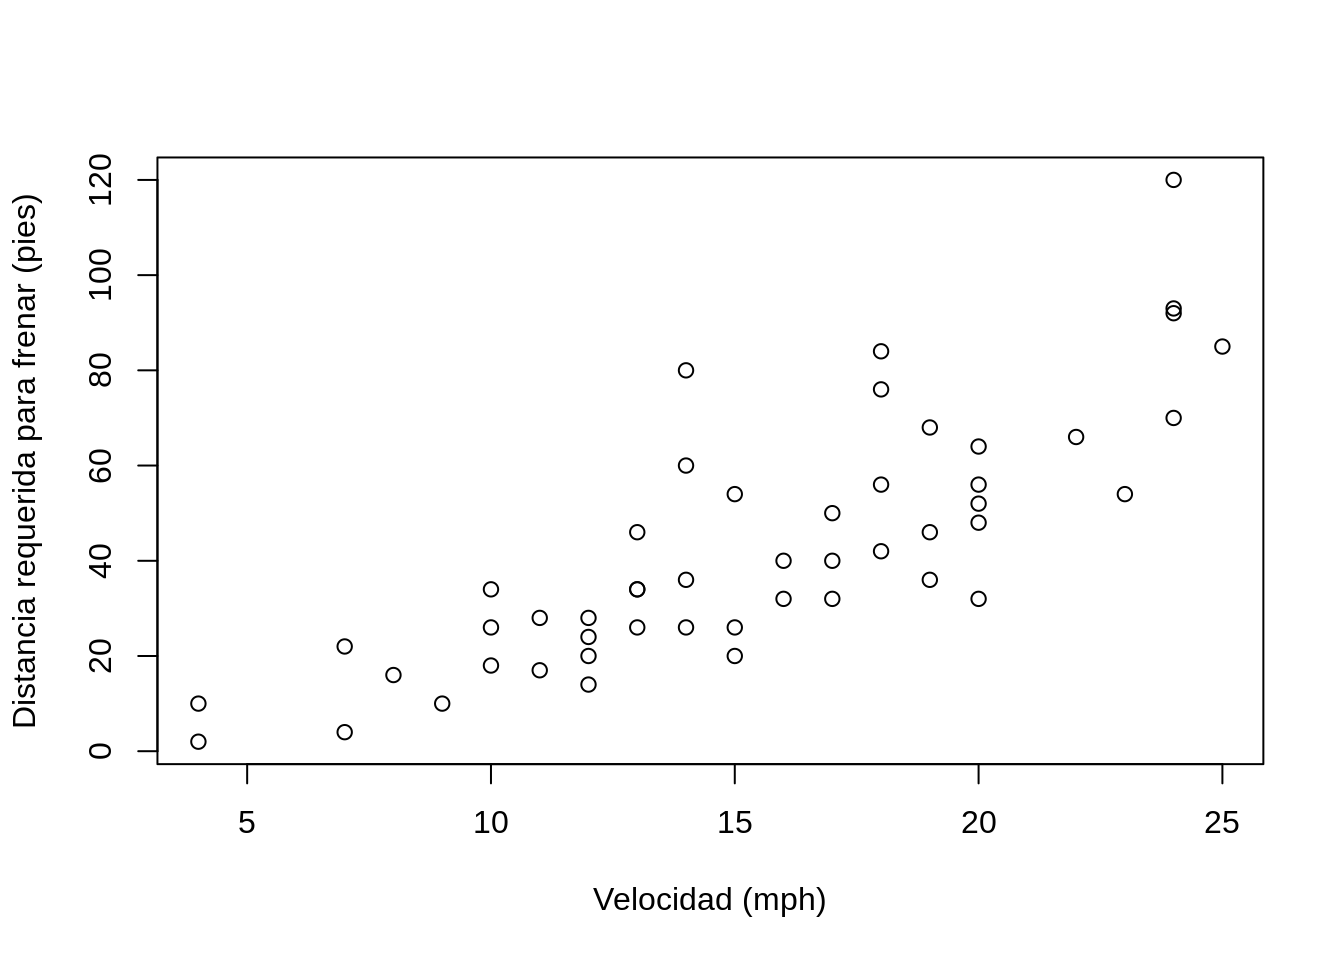
\includegraphics{./05-r-conceptos_basicos_files/figure-pdf/code-argumentos-1.pdf}

}

\end{figure}

\hypertarget{ejercicios-2}{%
\subsection{Ejercicios}\label{ejercicios-2}}

\begin{enumerate}
\def\labelenumi{\arabic{enumi}.}
\tightlist
\item
  Estudie la documentación de la función \texttt{plot()} y agregue al
  gráfico anterior:

  \begin{enumerate}
  \def\labelenumii{\alph{enumii}.}
  \tightlist
  \item
    Un título.
  \item
    Un subtítulo.
  \end{enumerate}
\end{enumerate}

\hypertarget{ayuda}{%
\subsection{Ayuda}\label{ayuda}}

Para obtener ayuda sobre una función desde la línea de comandos de R,
puede utilizarse un signo de pregunta (\texttt{?}) seguido del nombre de
la función o bien la función
\href{https://rdrr.io/r/utils/help.html}{help()}. Por ejemplo:

\begin{Shaded}
\begin{Highlighting}[]
\CommentTok{\# Ayuda de la función setwd()}
\NormalTok{?setwd}
\FunctionTok{help}\NormalTok{(setwd)}
\end{Highlighting}
\end{Shaded}

También puede utilizarse la función
\href{https://rdrr.io/r/utils/apropos.html}{apropos()}, para buscar
funciones por palabras clave.

\begin{Shaded}
\begin{Highlighting}[]
\CommentTok{\# Búsqueda, por palabras clave, de funciones relacionadas con "mean" (media aritmética). Note las comillas ("").}
\FunctionTok{apropos}\NormalTok{(}\StringTok{"mean"}\NormalTok{)}
\end{Highlighting}
\end{Shaded}

\begin{verbatim}
 [1] ".colMeans"     ".rowMeans"     "colMeans"      "kmeans"       
 [5] "mean"          "mean.Date"     "mean.default"  "mean.difftime"
 [9] "mean.POSIXct"  "mean.POSIXlt"  "rowMeans"      "weighted.mean"
\end{verbatim}

La función \href{https://rdrr.io/r/utils/example.html}{example()}
presenta ejemplos sobre el uso de una función.

\begin{Shaded}
\begin{Highlighting}[]
\CommentTok{\# Ejemplos de uso de la función mean()}
\FunctionTok{example}\NormalTok{(}\StringTok{"mean"}\NormalTok{)}
\end{Highlighting}
\end{Shaded}

\begin{verbatim}

mean> x <- c(0:10, 50)

mean> xm <- mean(x)

mean> c(xm, mean(x, trim = 0.10))
[1] 8.75 5.50
\end{verbatim}

Por otra parte, el sitio \href{https://rdrr.io/r/}{All R Documentation}
reúne documentación de funciones de una gran cantidad de paquetes de R.

También puede obtenerse ayuda en buscadores de Internet, como
\href{https://www.google.com/}{Google}, o en sitios de preguntas y
respuestas para programadores, como
\href{https://stackoverflow.com/}{Stack Overflow}.

\hypertarget{paquetes}{%
\section{Paquetes}\label{paquetes}}

Las funciones de R se distribuyen en
\href{https://en.wikipedia.org/wiki/R_package}{paquetes}. Cada paquete
contiene un conjunto de funciones y estructuras de datos relacionadas
entre sí. También hay paquetes que contienen datos.

Para utilizar un paquete, primero debe cargarse (en la memoria del
computador) con la función
\href{https://rdrr.io/r/base/library.html}{library()}.

\begin{Shaded}
\begin{Highlighting}[]
\CommentTok{\# Carga del paquete stats}
\FunctionTok{library}\NormalTok{(stats)}
\end{Highlighting}
\end{Shaded}

Algunos paquetes están contenidos en la distribución base de R. Otros
deben instalarse con la función
\href{https://rdrr.io/r/utils/install.packages.html}{install.packages()}.

En el siguiente ejemplo, se instala el paquete
\href{https://cran.r-project.org/package=PASWR2}{PASWR2}, el cual
contiene el conjunto de datos
\href{https://rdrr.io/cran/PASWR2/man/TITANIC3.html}{TITANIC3} con una
lista de pasajeros del
\href{https://es.wikipedia.org/wiki/RMS_Titanic}{Titanic}.

\begin{Shaded}
\begin{Highlighting}[]
\CommentTok{\# Instalación del paquete PASWR2 (note las comillas)}
\FunctionTok{install.packages}\NormalTok{(}\StringTok{"PASWR2"}\NormalTok{)}
\end{Highlighting}
\end{Shaded}

Seguidamente, el paquete \texttt{PASWR2} se carga con la función
\texttt{library()}.

\begin{Shaded}
\begin{Highlighting}[]
\CommentTok{\# Carga de PASWR2}
\FunctionTok{library}\NormalTok{(PASWR2)}
\end{Highlighting}
\end{Shaded}

El conjunto de datos \texttt{TITANIC3} puede visualizarse con la función
\href{https://rdrr.io/r/utils/View.html}{View()}.

\begin{Shaded}
\begin{Highlighting}[]
\CommentTok{\# Visualización del conjunto de datos TITANIC3}
\FunctionTok{View}\NormalTok{(TITANIC3)}
\end{Highlighting}
\end{Shaded}

El siguiente
\href{https://es.wikipedia.org/wiki/Diagrama_de_barras}{gráfico de
barras} muestra la distribución de pasajeros por clase, mediante la
función \href{https://rdrr.io/r/graphics/barplot.html}{barplot()}.
También se utiliza la función
\href{https://rdrr.io/r/base/table.html}{table()} para generar una tabla
con las cantidades de pasajeros que viajaban en cada clase.

\begin{Shaded}
\begin{Highlighting}[]
\CommentTok{\# Cantidades de pasajeros por clase}
\FunctionTok{table}\NormalTok{(TITANIC3}\SpecialCharTok{$}\NormalTok{pclass)}
\DocumentationTok{\#\# }
\DocumentationTok{\#\# 1st 2nd 3rd }
\DocumentationTok{\#\# 323 277 709}

\CommentTok{\# Gráfico de barras por clase de pasajero}
\FunctionTok{barplot}\NormalTok{(}
  \AttributeTok{height=}\FunctionTok{table}\NormalTok{(TITANIC3}\SpecialCharTok{$}\NormalTok{pclass),}
  \AttributeTok{main=}\StringTok{"Distribución de pasajeros del Titanic por clase"}\NormalTok{,}
  \AttributeTok{xlab =} \StringTok{"Clase"}\NormalTok{,}
  \AttributeTok{ylab =} \StringTok{"Cantidad de pasajeros"}  
\NormalTok{)}
\end{Highlighting}
\end{Shaded}

\begin{figure}[H]

{\centering 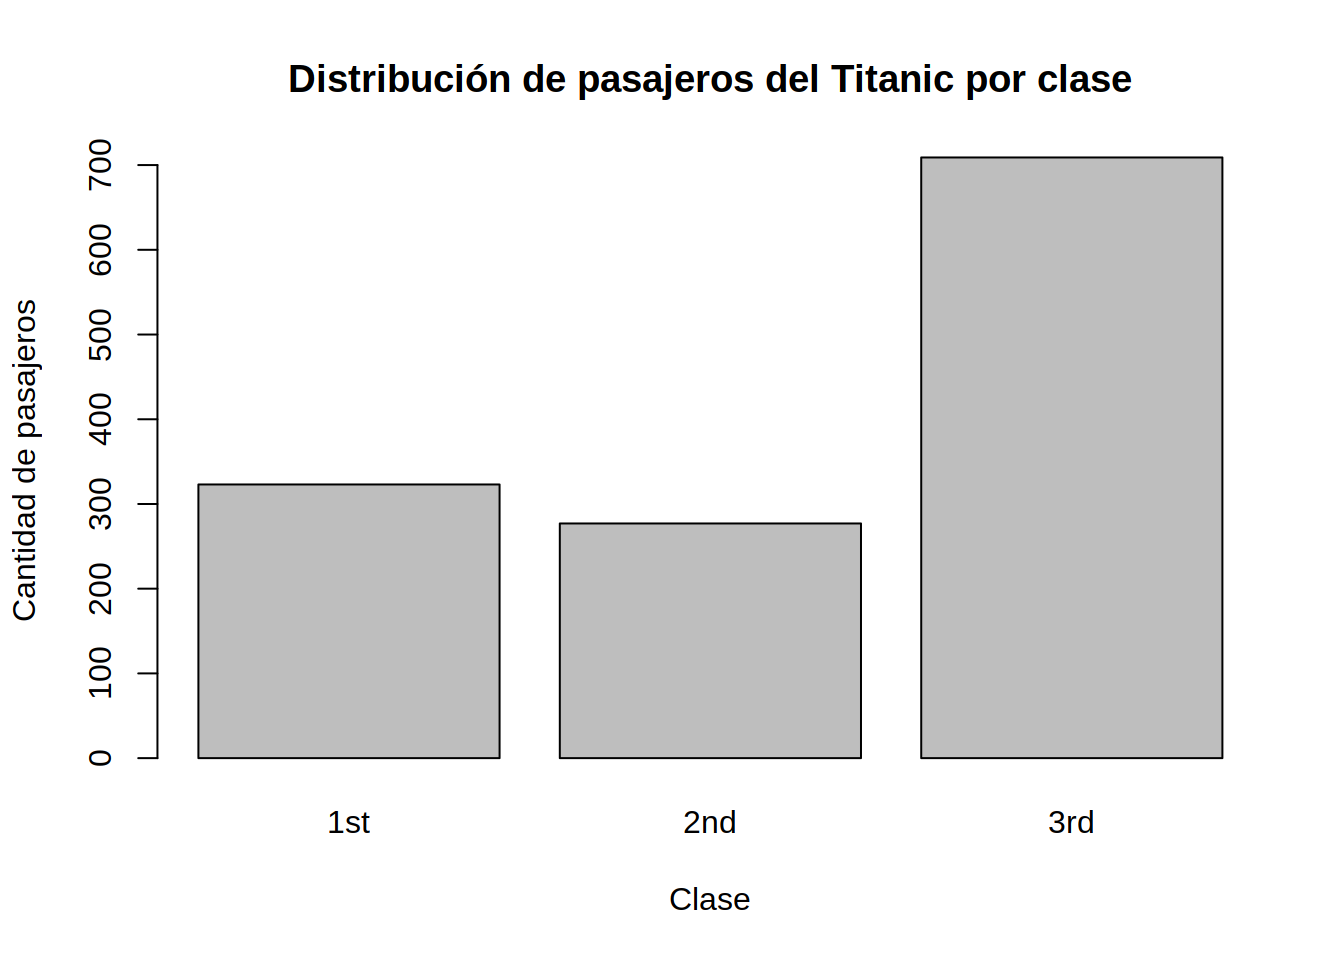
\includegraphics{./05-r-conceptos_basicos_files/figure-pdf/code-titanic-barplot-clase-1.pdf}

}

\end{figure}

La distribución por cada clase puede dividirse en fallecidos y
sobrevivientes.

\begin{Shaded}
\begin{Highlighting}[]
\CommentTok{\# Cantidades de pasajeros fallecidos y sobrevivientes por clase}
\CommentTok{\# (0 corresponde a fallecidos y 1 a sobrevivientes)}
\FunctionTok{table}\NormalTok{(TITANIC3}\SpecialCharTok{$}\NormalTok{survived, TITANIC3}\SpecialCharTok{$}\NormalTok{pclass)}
\DocumentationTok{\#\#    }
\DocumentationTok{\#\#     1st 2nd 3rd}
\DocumentationTok{\#\#   0 123 158 528}
\DocumentationTok{\#\#   1 200 119 181}
\end{Highlighting}
\end{Shaded}

El siguiente gráfico muestra en un gráfico de barras apiladas la
distribución de pasajeros sobrevivientes y fallecidos en cada clase.

\begin{Shaded}
\begin{Highlighting}[]
\CommentTok{\# Gráfico de barras apiladas}
\FunctionTok{barplot}\NormalTok{(}
  \AttributeTok{height =} \FunctionTok{table}\NormalTok{(TITANIC3}\SpecialCharTok{$}\NormalTok{survived, TITANIC3}\SpecialCharTok{$}\NormalTok{pclass),}
  \AttributeTok{main =} \StringTok{"Distribución de pasajeros fallecidos y sobrevivientes por clase"}\NormalTok{,}
  \AttributeTok{xlab =} \StringTok{"Clase"}\NormalTok{,}
  \AttributeTok{ylab =} \StringTok{"Cantidad de pasajeros"}\NormalTok{,}
  \AttributeTok{col =} \FunctionTok{topo.colors}\NormalTok{(}\DecValTok{2}\NormalTok{)}
\NormalTok{)}

\CommentTok{\# Leyenda}
\FunctionTok{legend}\NormalTok{(}
  \AttributeTok{x =} \StringTok{"topleft"}\NormalTok{,}
  \AttributeTok{inset =} \FloatTok{0.03}\NormalTok{,}
  \AttributeTok{legend =} \FunctionTok{c}\NormalTok{(}\StringTok{"Fallecidos"}\NormalTok{, }\StringTok{"Sobrevivientes"}\NormalTok{),}
  \AttributeTok{fill =} \FunctionTok{topo.colors}\NormalTok{(}\DecValTok{2}\NormalTok{),}
  \AttributeTok{horiz =} \ConstantTok{TRUE}
\NormalTok{)}
\end{Highlighting}
\end{Shaded}

\begin{figure}[H]

{\centering 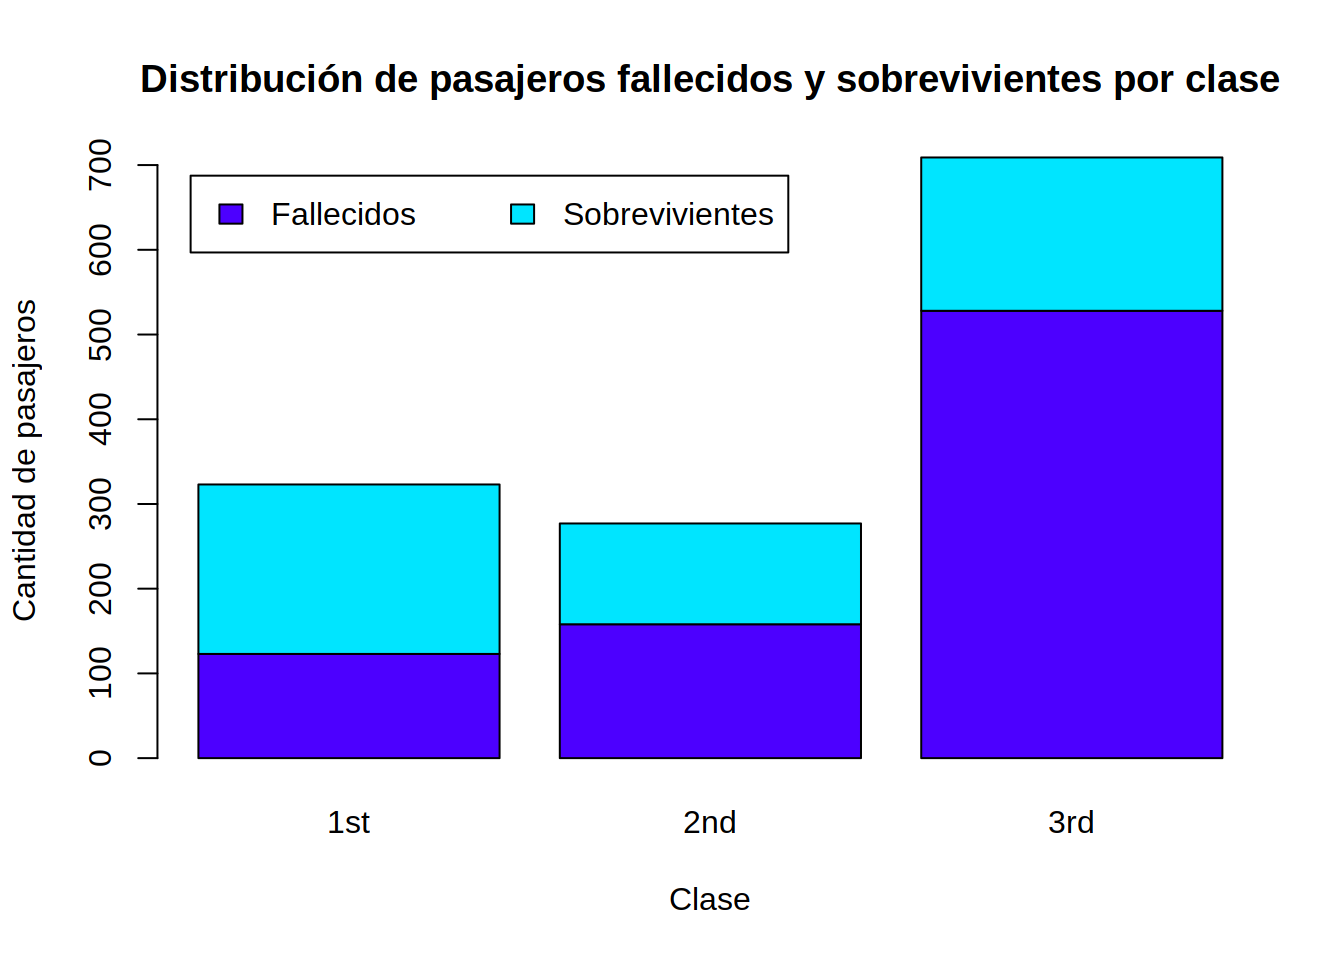
\includegraphics{./05-r-conceptos_basicos_files/figure-pdf/code-titanic-barplot-stacked-sobrevivientes-clase-1.pdf}

}

\end{figure}

La misma información se muestra seguidamente en un gráfico de barras
agrupadas. Note el uso del argumento \texttt{beside}.

\begin{Shaded}
\begin{Highlighting}[]
\CommentTok{\# Gráfico de barras agrupadas}
\FunctionTok{barplot}\NormalTok{(}
  \AttributeTok{height =} \FunctionTok{table}\NormalTok{(TITANIC3}\SpecialCharTok{$}\NormalTok{survived, TITANIC3}\SpecialCharTok{$}\NormalTok{pclass),}
  \AttributeTok{main =} \StringTok{"Distribución de pasajeros fallecidos y sobrevivientes por clase"}\NormalTok{,}
  \AttributeTok{xlab =} \StringTok{"Clase"}\NormalTok{,}
  \AttributeTok{ylab =} \StringTok{"Cantidad de pasajeros"}\NormalTok{,  }
  \AttributeTok{col =} \FunctionTok{topo.colors}\NormalTok{(}\DecValTok{2}\NormalTok{),}
  \AttributeTok{beside =} \ConstantTok{TRUE}
\NormalTok{)}

\CommentTok{\# Leyenda}
\FunctionTok{legend}\NormalTok{(}
  \AttributeTok{x =} \StringTok{"topleft"}\NormalTok{,}
  \AttributeTok{inset =} \FloatTok{0.03}\NormalTok{,}
  \AttributeTok{legend =} \FunctionTok{c}\NormalTok{(}\StringTok{"Fallecidos"}\NormalTok{, }\StringTok{"Sobrevivientes"}\NormalTok{),}
  \AttributeTok{fill =} \FunctionTok{topo.colors}\NormalTok{(}\DecValTok{2}\NormalTok{),}
  \AttributeTok{horiz =} \ConstantTok{TRUE}
\NormalTok{)}
\end{Highlighting}
\end{Shaded}

\begin{figure}[H]

{\centering 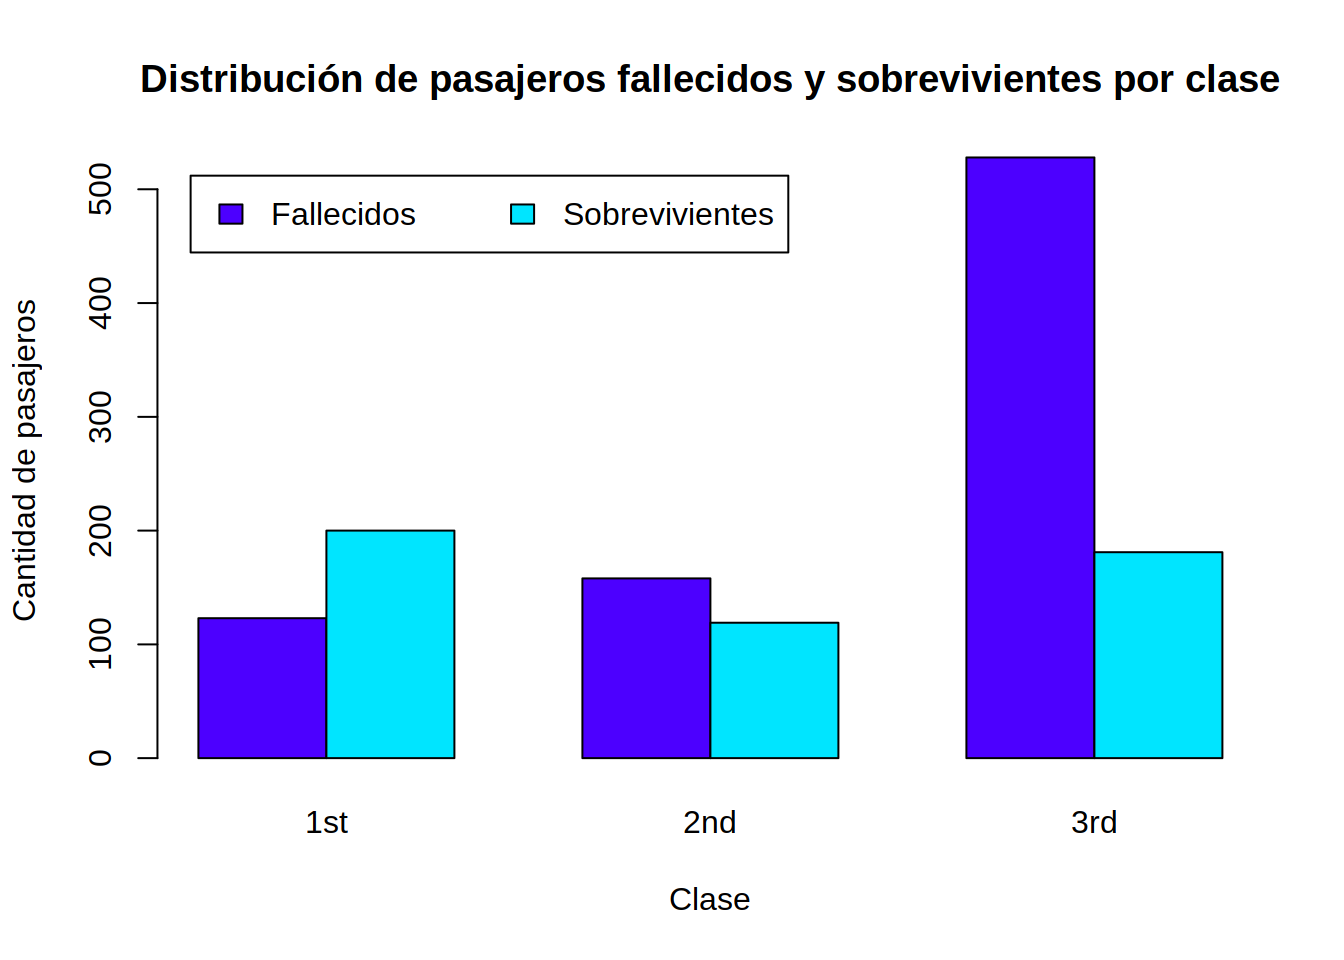
\includegraphics{./05-r-conceptos_basicos_files/figure-pdf/code-titanic-barplot-grouped-sobrevivientes-clase-1.pdf}

}

\end{figure}

\hypertarget{ejercicios-3}{%
\subsection{Ejercicios}\label{ejercicios-3}}

\begin{enumerate}
\def\labelenumi{\arabic{enumi}.}
\tightlist
\item
  Muestre la distribución de pasajeros fallecidos y sobrevivientes por
  sexo en un gráfico de barras apiladas.
\item
  Muestre la distribución de pasajeros fallecidos y sobrevivientes por
  sexo en un gráfico de barras agrupadas.
\end{enumerate}

\hypertarget{tipos-de-datos}{%
\section{Tipos de datos}\label{tipos-de-datos}}

R puede trabajar con varios
\href{https://cran.r-project.org/doc/manuals/r-release/R-lang.html\#Basic-types}{tipos
de datos básicos}, entre los que están números, caracteres (i.e.~textos)
y lógicos. También puede trabajar con
\href{https://cran.r-project.org/doc/manuals/r-release/R-lang.html\#Special-compound-objects}{tipos
compuestos}, como factores y \emph{data frames}.

R proporciona acceso a los datos a través de objetos. Un objeto es una
entidad que tiene asociadas propiedades (i.e.~datos) y métodos
(i.e.~funciones) para manipular esas propiedades. Un objeto puede ser,
por ejemplo, un número, una hilera de texto, un vector o una matriz. R
también permite que el programador defina sus propios objetos.

Hay muchas formas de crear objetos en R. Una de las más sencillas es con
los operadores de asignación. Estos son \texttt{=} y
\texttt{\textless{}-} (o \texttt{-\textgreater{}}). Por ejemplo, las
siguientes sentencias crean un número, un texto y un vector.

\begin{Shaded}
\begin{Highlighting}[]
\CommentTok{\# Número}
\NormalTok{x }\OtherTok{\textless{}{-}} \DecValTok{10}
\NormalTok{x}
\DocumentationTok{\#\# [1] 10}

\CommentTok{\# Otro número}
\DecValTok{20} \OtherTok{{-}\textgreater{}}\NormalTok{ y}
\NormalTok{y}
\DocumentationTok{\#\# [1] 20}

\CommentTok{\# Hilera de caracteres}
\NormalTok{nombre }\OtherTok{\textless{}{-}} \StringTok{\textquotesingle{}Manuel\textquotesingle{}}
\NormalTok{nombre}
\DocumentationTok{\#\# [1] "Manuel"}

\CommentTok{\# Vector de hileras de caracteres}
\NormalTok{dias }\OtherTok{\textless{}{-}} \FunctionTok{c}\NormalTok{(}\StringTok{\textquotesingle{}Domingo\textquotesingle{}}\NormalTok{, }\StringTok{\textquotesingle{}Lunes\textquotesingle{}}\NormalTok{, }\StringTok{\textquotesingle{}Martes\textquotesingle{}}\NormalTok{, }\StringTok{\textquotesingle{}Miércoles\textquotesingle{}}\NormalTok{, }\StringTok{\textquotesingle{}Jueves\textquotesingle{}}\NormalTok{, }\StringTok{\textquotesingle{}Viernes\textquotesingle{}}\NormalTok{, }\StringTok{\textquotesingle{}Sábado\textquotesingle{}}\NormalTok{)}
\NormalTok{dias}
\DocumentationTok{\#\# [1] "Domingo"   "Lunes"     "Martes"    "Miércoles" "Jueves"    "Viernes"  }
\DocumentationTok{\#\# [7] "Sábado"}
\end{Highlighting}
\end{Shaded}

Tanto \texttt{x}, como \texttt{nombre} como \texttt{dias} son variables.
Una variable es una etiqueta que se le asigna a un objeto. Una variable
debe comenzar con una letra.

El tipo de un objeto puede consultarse con la función
\href{https://rdrr.io/r/base/typeof.html}{typeof()}. Por ejemplo:

\begin{Shaded}
\begin{Highlighting}[]
\FunctionTok{typeof}\NormalTok{(x)}
\DocumentationTok{\#\# [1] "double"}
\FunctionTok{typeof}\NormalTok{(y)}
\DocumentationTok{\#\# [1] "double"}
\FunctionTok{typeof}\NormalTok{(nombre)}
\DocumentationTok{\#\# [1] "character"}
\FunctionTok{typeof}\NormalTok{(dias)}
\DocumentationTok{\#\# [1] "character"}
\end{Highlighting}
\end{Shaded}

A continuación, se describen con más detalle algunos de los tipos de
datos utilizados en el lenguaje R.

\hypertarget{tipos-buxe1sicos}{%
\subsection{Tipos básicos}\label{tipos-buxe1sicos}}

R define
\href{https://cran.r-project.org/doc/manuals/r-release/R-lang.html\#Basic-types}{seis
tipos de datos básicos}. En esta sección, se describen los más
utilizados durante este curso.

\hypertarget{nuxfameros}{%
\subsubsection{Números}\label{nuxfameros}}

Pueden ser enteros (\texttt{integer}) o decimales (\texttt{double}). Se
utilizan en diversos tipos de operaciones, incluyendo las aritméticas
(ej. suma, resta, multiplicación, división).

\begin{Shaded}
\begin{Highlighting}[]
\CommentTok{\# Declaración de variables numéricas}
\NormalTok{x }\OtherTok{\textless{}{-}} \DecValTok{5}
\NormalTok{y }\OtherTok{\textless{}{-}} \FloatTok{0.5}

\CommentTok{\# Suma}
\NormalTok{x }\SpecialCharTok{+}\NormalTok{ y}
\DocumentationTok{\#\# [1] 5.5}

\CommentTok{\# Tipos de datos numéricos}
\FunctionTok{typeof}\NormalTok{(x)}
\DocumentationTok{\#\# [1] "double"}
\FunctionTok{typeof}\NormalTok{(y)}
\DocumentationTok{\#\# [1] "double"}
\FunctionTok{typeof}\NormalTok{(x }\SpecialCharTok{+}\NormalTok{ y)}
\DocumentationTok{\#\# [1] "double"}
\end{Highlighting}
\end{Shaded}

Nótese que al declararse una variable numérica, ya sea que tenga o no
punto decimal, R la considera por defecto de tipo \texttt{double}. Para
que se considere de tipo \texttt{integer}, debe utilizarse el sufijo
\texttt{L} o la función \texttt{as.integer()}.

\begin{Shaded}
\begin{Highlighting}[]
\CommentTok{\# Números enteros}
\NormalTok{x }\OtherTok{\textless{}{-}}\NormalTok{ 10L}
\NormalTok{y }\OtherTok{\textless{}{-}} \FunctionTok{as.integer}\NormalTok{(}\DecValTok{15}\NormalTok{)}

\CommentTok{\# Multiplicación}
\NormalTok{x }\SpecialCharTok{*}\NormalTok{ y}
\DocumentationTok{\#\# [1] 150}

\CommentTok{\# Tipos de datos enteros}
\FunctionTok{typeof}\NormalTok{(x)}
\DocumentationTok{\#\# [1] "integer"}
\FunctionTok{typeof}\NormalTok{(y)}
\DocumentationTok{\#\# [1] "integer"}
\FunctionTok{typeof}\NormalTok{(x }\SpecialCharTok{*}\NormalTok{ y)}
\DocumentationTok{\#\# [1] "integer"}
\end{Highlighting}
\end{Shaded}

\hypertarget{caracteres}{%
\subsubsection{Caracteres}\label{caracteres}}

Se utilizan para representar textos. Deben estar entre comillas simples
(\texttt{\textquotesingle{}\textquotesingle{}}) o dobles (\texttt{""}).

\begin{Shaded}
\begin{Highlighting}[]
\CommentTok{\# Hileras de caracteres}
\NormalTok{nombre }\OtherTok{\textless{}{-}} \StringTok{"María"}
\NormalTok{apellido }\OtherTok{\textless{}{-}} \StringTok{"Pérez"}

\CommentTok{\# Concatenación mediante la función paste()}
\FunctionTok{paste}\NormalTok{(nombre, apellido)}
\DocumentationTok{\#\# [1] "María Pérez"}
\end{Highlighting}
\end{Shaded}

\hypertarget{luxf3gicos}{%
\subsubsection{Lógicos}\label{luxf3gicos}}

Los objetos lógicos (también llamados \emph{booleanos}) tienen dos
posibles valores: verdadero (\texttt{TRUE}) o falso (\texttt{FALSE}).

\begin{Shaded}
\begin{Highlighting}[]
\CommentTok{\# Variable lógica}
\NormalTok{a }\OtherTok{\textless{}{-}} \DecValTok{1} \SpecialCharTok{\textless{}} \DecValTok{2}
\NormalTok{a}
\DocumentationTok{\#\# [1] TRUE}

\CommentTok{\# Variable lógica}
\NormalTok{b }\OtherTok{\textless{}{-}} \DecValTok{1} \SpecialCharTok{\textgreater{}} \DecValTok{2}
\NormalTok{b}
\DocumentationTok{\#\# [1] FALSE}
\end{Highlighting}
\end{Shaded}

Las expresiones lógicas pueden combinarse con operadores como:

\begin{itemize}
\tightlist
\item
  \texttt{\&} (Y, en inglés \emph{AND})
\item
  \texttt{\textbar{}} (O, en inglés \emph{OR})
\item
  \texttt{!} (NO, en inglés \emph{NOT})
\end{itemize}

\begin{Shaded}
\begin{Highlighting}[]
\CommentTok{\# Operador lógico AND}
\NormalTok{(}\DecValTok{1} \SpecialCharTok{\textless{}} \DecValTok{2}\NormalTok{) }\SpecialCharTok{\&}\NormalTok{ (}\DecValTok{3} \SpecialCharTok{\textless{}} \DecValTok{4}\NormalTok{)}
\DocumentationTok{\#\# [1] TRUE}

\CommentTok{\# Operador lógico OR}
\NormalTok{(}\DecValTok{2} \SpecialCharTok{+} \DecValTok{2} \SpecialCharTok{==} \DecValTok{5}\NormalTok{) }\SpecialCharTok{|}\NormalTok{ (}\DecValTok{20} \SpecialCharTok{\textless{}=} \DecValTok{10}\NormalTok{)}
\DocumentationTok{\#\# [1] FALSE}

\CommentTok{\# Operador lógico NOT}
\SpecialCharTok{!}\NormalTok{(}\DecValTok{2} \SpecialCharTok{+} \DecValTok{2} \SpecialCharTok{==} \DecValTok{5}\NormalTok{)}
\DocumentationTok{\#\# [1] TRUE}
\end{Highlighting}
\end{Shaded}

\hypertarget{vectores}{%
\subsubsection{Vectores}\label{vectores}}

Un
\href{https://cran.r-project.org/doc/manuals/r-release/R-lang.html\#Vector-objects}{vector}
es una estructura unidimensional que combina objetos del mismo tipo.

\hypertarget{definiciuxf3n}{%
\paragraph{Definición}\label{definiciuxf3n}}

Los vectores pueden definirse de varias formas como, por ejemplo, con la
función \href{https://rdrr.io/r/base/c.html}{c()} (del inglés
\emph{combine}):

\begin{Shaded}
\begin{Highlighting}[]
\CommentTok{\# Definición de un vector de números}
\NormalTok{vector\_numeros }\OtherTok{\textless{}{-}} \FunctionTok{c}\NormalTok{(}\DecValTok{1}\NormalTok{, }\DecValTok{7}\NormalTok{, }\DecValTok{32}\NormalTok{, }\DecValTok{45}\NormalTok{, }\DecValTok{57}\NormalTok{)}
\NormalTok{vector\_numeros}
\DocumentationTok{\#\# [1]  1  7 32 45 57}

\CommentTok{\# Definición de un vector de hileras de caracteres}
\NormalTok{vector\_nombres }\OtherTok{\textless{}{-}} \FunctionTok{c}\NormalTok{(}\StringTok{"Álvaro"}\NormalTok{, }\StringTok{"Ana"}\NormalTok{, }\StringTok{"Berta"}\NormalTok{, }\StringTok{"Bernardo"}\NormalTok{)}
\NormalTok{vector\_nombres}
\DocumentationTok{\#\# [1] "Álvaro"   "Ana"      "Berta"    "Bernardo"}
\end{Highlighting}
\end{Shaded}

Los vectores también pueden crearse con el operador \texttt{:}, el cual
especifica una secuencia (i.e.~una lista ordenada):

\begin{Shaded}
\begin{Highlighting}[]
\CommentTok{\# Definición de un vector de números con la secuencia de 1 a 10}
\NormalTok{vector\_secuencia }\OtherTok{\textless{}{-}} \DecValTok{1}\SpecialCharTok{:}\DecValTok{10}
\NormalTok{vector\_secuencia}
\DocumentationTok{\#\#  [1]  1  2  3  4  5  6  7  8  9 10}

\CommentTok{\# Definición de un vector de números con la secuencia de {-}5 a 5}
\NormalTok{vector\_secuencia }\OtherTok{\textless{}{-}} \SpecialCharTok{{-}}\DecValTok{5}\SpecialCharTok{:}\DecValTok{5}
\NormalTok{vector\_secuencia}
\DocumentationTok{\#\#  [1] {-}5 {-}4 {-}3 {-}2 {-}1  0  1  2  3  4  5}

\CommentTok{\# Definición de un vector de números con la secuencia de {-}0.5 a 3.7}
\NormalTok{vector\_secuencia }\OtherTok{\textless{}{-}} \SpecialCharTok{{-}}\FloatTok{0.5}\SpecialCharTok{:}\FloatTok{3.7}
\NormalTok{vector\_secuencia}
\DocumentationTok{\#\# [1] {-}0.5  0.5  1.5  2.5  3.5}
\end{Highlighting}
\end{Shaded}

La función \href{https://rdrr.io/r/base/seq.html}{seq()} también crea un
vector con base en una secuencia y permite especificar argumentos como
un valor de incremento y la longitud de la secuencia.

\begin{Shaded}
\begin{Highlighting}[]
\CommentTok{\# Definición de un vector de números en secuencia de 1 a 10}
\NormalTok{vector\_secuencia }\OtherTok{\textless{}{-}} \FunctionTok{seq}\NormalTok{(}\DecValTok{1}\NormalTok{, }\DecValTok{10}\NormalTok{)}
\NormalTok{vector\_secuencia}
\DocumentationTok{\#\#  [1]  1  2  3  4  5  6  7  8  9 10}

\CommentTok{\# Definición de un vector de números en secuencia de 0.5 a 15.3, con incremento de 2}
\NormalTok{vector\_secuencia }\OtherTok{\textless{}{-}} \FunctionTok{seq}\NormalTok{(}\AttributeTok{from=}\FloatTok{0.5}\NormalTok{, }\AttributeTok{to=}\FloatTok{15.3}\NormalTok{, }\AttributeTok{by=}\DecValTok{2}\NormalTok{)}
\NormalTok{vector\_secuencia}
\DocumentationTok{\#\# [1]  0.5  2.5  4.5  6.5  8.5 10.5 12.5 14.5}

\CommentTok{\# Definición de un vector de números en secuencia de 1.5 a 9.4, con longitud de 4}
\NormalTok{vector\_secuencia }\OtherTok{\textless{}{-}} \FunctionTok{seq}\NormalTok{(}\AttributeTok{from=}\FloatTok{1.5}\NormalTok{, }\AttributeTok{to=}\FloatTok{9.4}\NormalTok{, }\AttributeTok{length.out=}\DecValTok{4}\NormalTok{)}
\NormalTok{vector\_secuencia}
\DocumentationTok{\#\# [1] 1.500000 4.133333 6.766667 9.400000}
\end{Highlighting}
\end{Shaded}

\hypertarget{indexaciuxf3n}{%
\paragraph{Indexación}\label{indexaciuxf3n}}

Los elementos de un vector se acceden a través de sus
\href{https://cran.r-project.org/doc/manuals/r-release/R-lang.html\#Indexing}{índices}
(i.e.~posiciones). La primera posición corresponde al índice 1, la
segunda al índice 2 y así sucesivamente. Los índices se especifican
entre paréntesis cuadrados (\texttt{{[}{]}}), ya sea para una posición
específica o para un rango de posiciones. También es posible especificar
los índices que se desea excluir.

\begin{Shaded}
\begin{Highlighting}[]
\CommentTok{\# Vector de nombres de países}
\NormalTok{paises }\OtherTok{\textless{}{-}} \FunctionTok{c}\NormalTok{(}\StringTok{"Argentina"}\NormalTok{, }\StringTok{"Francia"}\NormalTok{, }\StringTok{"China"}\NormalTok{, }\StringTok{"Australia"}\NormalTok{, }\StringTok{"México"}\NormalTok{)}
\NormalTok{paises}
\DocumentationTok{\#\# [1] "Argentina" "Francia"   "China"     "Australia" "México"}

\CommentTok{\# Elemento en el índice 3}
\NormalTok{paises[}\DecValTok{3}\NormalTok{]}
\DocumentationTok{\#\# [1] "China"}
\end{Highlighting}
\end{Shaded}

El operador \texttt{:} puede utilizarse para especificar un rango de
índices:

\begin{Shaded}
\begin{Highlighting}[]
\CommentTok{\# Elementos entre los índices 2 y 4 (2, 3 y 4)}
\NormalTok{paises[}\DecValTok{2}\SpecialCharTok{:}\DecValTok{4}\NormalTok{]}
\DocumentationTok{\#\# [1] "Francia"   "China"     "Australia"}
\end{Highlighting}
\end{Shaded}

Con la función \texttt{c()}, es posible especificar un conjunto de
índices particulares:

\begin{Shaded}
\begin{Highlighting}[]
\CommentTok{\# Elementos entre los índices 1, 4 y 5}
\NormalTok{paises[}\FunctionTok{c}\NormalTok{(}\DecValTok{1}\NormalTok{, }\DecValTok{4}\NormalTok{, }\DecValTok{5}\NormalTok{)]}
\DocumentationTok{\#\# [1] "Argentina" "Australia" "México"}
\end{Highlighting}
\end{Shaded}

Los números negativos pueden usarse para excluir índices:

\begin{Shaded}
\begin{Highlighting}[]
\CommentTok{\# Exclusión de los índices 3 y 4}
\NormalTok{paises[}\FunctionTok{c}\NormalTok{(}\SpecialCharTok{{-}}\DecValTok{3}\NormalTok{, }\SpecialCharTok{{-}}\DecValTok{4}\NormalTok{)]}
\DocumentationTok{\#\# [1] "Argentina" "Francia"   "México"}
\end{Highlighting}
\end{Shaded}

Los valores lógicos \texttt{TRUE} y \texttt{FALSE} también pueden usarse
para incluir y excluir índices de un vector:

\begin{Shaded}
\begin{Highlighting}[]
\CommentTok{\# Se incluyen los índices 1, 2 y 4; y se excluyen los índices 3 y 5}
\NormalTok{paises[}\FunctionTok{c}\NormalTok{(}\ConstantTok{TRUE}\NormalTok{, }\ConstantTok{TRUE}\NormalTok{, }\ConstantTok{FALSE}\NormalTok{, }\ConstantTok{TRUE}\NormalTok{, }\ConstantTok{FALSE}\NormalTok{)]}
\DocumentationTok{\#\# [1] "Argentina" "Francia"   "Australia"}
\end{Highlighting}
\end{Shaded}

\hypertarget{operaciones}{%
\paragraph{Operaciones}\label{operaciones}}

En los vectores pueden aplicarse operaciones aritméticas:

\begin{Shaded}
\begin{Highlighting}[]
\NormalTok{a }\OtherTok{\textless{}{-}} \FunctionTok{c}\NormalTok{(}\DecValTok{1}\NormalTok{, }\DecValTok{3}\NormalTok{, }\DecValTok{5}\NormalTok{, }\DecValTok{7}\NormalTok{)}
\NormalTok{b }\OtherTok{\textless{}{-}} \FunctionTok{c}\NormalTok{(}\DecValTok{2}\NormalTok{, }\DecValTok{4}\NormalTok{, }\DecValTok{6}\NormalTok{, }\DecValTok{8}\NormalTok{)}

\CommentTok{\# Suma de vectores}
\NormalTok{a }\SpecialCharTok{+}\NormalTok{ b}
\DocumentationTok{\#\# [1]  3  7 11 15}

\CommentTok{\# Multiplicación de vectores}
\NormalTok{a }\SpecialCharTok{*}\NormalTok{ b}
\DocumentationTok{\#\# [1]  2 12 30 56}
\end{Highlighting}
\end{Shaded}

Y también pueden realizarse operaciones relacionales:

\begin{Shaded}
\begin{Highlighting}[]
\CommentTok{\# Comparación con el operador \textless{}}
\NormalTok{a }\SpecialCharTok{\textless{}}\NormalTok{ b}
\DocumentationTok{\#\# [1] TRUE TRUE TRUE TRUE}
\end{Highlighting}
\end{Shaded}

\hypertarget{matrices}{%
\subsubsection{Matrices}\label{matrices}}

Una matriz es una estructura bidimensional de filas y columnas.

\hypertarget{definiciuxf3n-1}{%
\paragraph{Definición}\label{definiciuxf3n-1}}

Las matrices se definen mediante la función
\href{https://rdrr.io/r/base/matrix.html}{matrix()}.

\begin{Shaded}
\begin{Highlighting}[]
\CommentTok{\# Definición de una matriz de 3 x 3 con elementos de la secuencia 1:9 distribuidos en las columnas}
\NormalTok{m }\OtherTok{\textless{}{-}} \FunctionTok{matrix}\NormalTok{(}\DecValTok{1}\SpecialCharTok{:}\DecValTok{9}\NormalTok{, }\AttributeTok{nrow=}\DecValTok{3}\NormalTok{, }\AttributeTok{ncol=}\DecValTok{3}\NormalTok{)}
\NormalTok{m}
\DocumentationTok{\#\#      [,1] [,2] [,3]}
\DocumentationTok{\#\# [1,]    1    4    7}
\DocumentationTok{\#\# [2,]    2    5    8}
\DocumentationTok{\#\# [3,]    3    6    9}

\CommentTok{\# Definición de una matriz de 3 x 3 con elementos de la secuencia 1:9 distribuidos en las filas}
\NormalTok{m }\OtherTok{\textless{}{-}} \FunctionTok{matrix}\NormalTok{(}\DecValTok{1}\SpecialCharTok{:}\DecValTok{9}\NormalTok{, }\AttributeTok{nrow=}\DecValTok{3}\NormalTok{, }\AttributeTok{ncol=}\DecValTok{3}\NormalTok{, }\AttributeTok{byrow=}\ConstantTok{TRUE}\NormalTok{)}
\NormalTok{m}
\DocumentationTok{\#\#      [,1] [,2] [,3]}
\DocumentationTok{\#\# [1,]    1    2    3}
\DocumentationTok{\#\# [2,]    4    5    6}
\DocumentationTok{\#\# [3,]    7    8    9}

\CommentTok{\# Definición de una matriz de 3 x 2 con nombres para las filas y las columnas}
\NormalTok{datos }\OtherTok{\textless{}{-}} \FunctionTok{c}\NormalTok{(}\DecValTok{18}\NormalTok{, }\DecValTok{500}\NormalTok{, }\DecValTok{25}\NormalTok{, }\DecValTok{1000}\NormalTok{, }\DecValTok{30}\NormalTok{, }\DecValTok{2000}\NormalTok{)}
\NormalTok{filas }\OtherTok{\textless{}{-}} \FunctionTok{c}\NormalTok{(}\StringTok{"Ana"}\NormalTok{, }\StringTok{"Mario"}\NormalTok{, }\StringTok{"Laura"}\NormalTok{)}
\NormalTok{columnas }\OtherTok{\textless{}{-}} \FunctionTok{c}\NormalTok{(}\StringTok{"Edad"}\NormalTok{, }\StringTok{"Salario"}\NormalTok{)}

\NormalTok{m }\OtherTok{\textless{}{-}} \FunctionTok{matrix}\NormalTok{(datos, }\AttributeTok{nrow=}\DecValTok{3}\NormalTok{, }\AttributeTok{ncol=}\DecValTok{2}\NormalTok{, }\AttributeTok{byrow=}\ConstantTok{TRUE}\NormalTok{, }\AttributeTok{dimnames=}\FunctionTok{list}\NormalTok{(filas, columnas))}
\NormalTok{m}
\DocumentationTok{\#\#       Edad Salario}
\DocumentationTok{\#\# Ana     18     500}
\DocumentationTok{\#\# Mario   25    1000}
\DocumentationTok{\#\# Laura   30    2000}
\end{Highlighting}
\end{Shaded}

La función \href{https://rdrr.io/r/base/list.html}{list()} se utiliza,
en este caso, para combinar vectores. En general, se usa para combinar
datos de cualquier tipo.

\hypertarget{indexaciuxf3n-1}{%
\paragraph{Indexación}\label{indexaciuxf3n-1}}

La indexación de matrices es similar a la de vectores, pero deben
especificarse índices tanto para filas como para columnas.

\begin{Shaded}
\begin{Highlighting}[]
\CommentTok{\# Elemento en la posición [2,2] (segunda fila, segunda columna)}
\NormalTok{m[}\DecValTok{2}\NormalTok{, }\DecValTok{2}\NormalTok{]}
\DocumentationTok{\#\# [1] 1000}

\CommentTok{\# Elementos de la primera fila}
\NormalTok{m[}\DecValTok{1}\NormalTok{,]}
\DocumentationTok{\#\#    Edad Salario }
\DocumentationTok{\#\#      18     500}

\CommentTok{\# Elementos de la segunda columna}
\NormalTok{m[, }\DecValTok{2}\NormalTok{]}
\DocumentationTok{\#\#   Ana Mario Laura }
\DocumentationTok{\#\#   500  1000  2000}

\CommentTok{\# Elementos de las filas 1 y 2}
\NormalTok{m[}\DecValTok{1}\SpecialCharTok{:}\DecValTok{2}\NormalTok{, ]}
\DocumentationTok{\#\#       Edad Salario}
\DocumentationTok{\#\# Ana     18     500}
\DocumentationTok{\#\# Mario   25    1000}

\CommentTok{\# Elementos de la fila "Mario"}
\NormalTok{m[}\StringTok{"Mario"}\NormalTok{, ]}
\DocumentationTok{\#\#    Edad Salario }
\DocumentationTok{\#\#      25    1000}

\CommentTok{\# Elementos de la columna "Salario"}
\NormalTok{m[, }\StringTok{"Salario"}\NormalTok{]}
\DocumentationTok{\#\#   Ana Mario Laura }
\DocumentationTok{\#\#   500  1000  2000}
\end{Highlighting}
\end{Shaded}

\hypertarget{operaciones-1}{%
\paragraph{Operaciones}\label{operaciones-1}}

De manera similar a los vectores, en las matrices pueden realizarse
operaciones aritméticas y relacionales.

\begin{Shaded}
\begin{Highlighting}[]
\NormalTok{a }\OtherTok{\textless{}{-}} \FunctionTok{matrix}\NormalTok{(}\DecValTok{1}\SpecialCharTok{:}\DecValTok{4}\NormalTok{, }\AttributeTok{nrow=}\DecValTok{2}\NormalTok{, }\AttributeTok{ncol=}\DecValTok{2}\NormalTok{)}
\NormalTok{a}
\DocumentationTok{\#\#      [,1] [,2]}
\DocumentationTok{\#\# [1,]    1    3}
\DocumentationTok{\#\# [2,]    2    4}

\NormalTok{b }\OtherTok{\textless{}{-}} \FunctionTok{matrix}\NormalTok{(}\DecValTok{5}\SpecialCharTok{:}\DecValTok{8}\NormalTok{, }\AttributeTok{nrow=}\DecValTok{2}\NormalTok{, }\AttributeTok{ncol=}\DecValTok{2}\NormalTok{)}
\NormalTok{b}
\DocumentationTok{\#\#      [,1] [,2]}
\DocumentationTok{\#\# [1,]    5    7}
\DocumentationTok{\#\# [2,]    6    8}

\CommentTok{\# Suma de matrices}
\NormalTok{a }\SpecialCharTok{+}\NormalTok{ b}
\DocumentationTok{\#\#      [,1] [,2]}
\DocumentationTok{\#\# [1,]    6   10}
\DocumentationTok{\#\# [2,]    8   12}

\CommentTok{\# Multiplicación de matrices}
\NormalTok{a }\SpecialCharTok{*}\NormalTok{ b}
\DocumentationTok{\#\#      [,1] [,2]}
\DocumentationTok{\#\# [1,]    5   21}
\DocumentationTok{\#\# [2,]   12   32}

\CommentTok{\# Comparación de matrices con el operador \textgreater{}}
\NormalTok{a }\SpecialCharTok{\textgreater{}}\NormalTok{ b}
\DocumentationTok{\#\#       [,1]  [,2]}
\DocumentationTok{\#\# [1,] FALSE FALSE}
\DocumentationTok{\#\# [2,] FALSE FALSE}
\end{Highlighting}
\end{Shaded}

\hypertarget{tipos-compuestos}{%
\subsection{Tipos compuestos}\label{tipos-compuestos}}

\hypertarget{factores}{%
\subsubsection{Factores}\label{factores}}

Los
\href{https://cran.r-project.org/doc/manuals/r-release/R-lang.html\#Factors}{factores}
se utilizan para representar
\href{https://es.wikipedia.org/wiki/Variable_categ\%C3\%B3rica}{datos
categóricos}. Un factor corresponde a un conjunto de categorías
correspondientes a un concepto (ej. {[}``Sí'', ``No''{]}, {[}``Casado'',
``Soltero''{]}, {[}``Alto'', ``Medio'', ``Bajo''{]}).

Internamente, los factores se representan en R como números enteros con
etiquetas asociadas. A pesar de que los factores parecen (y pueden
funcionar como) hileras de caracteres, en realidad son números y debe
tenerse cuidado de no manejarlos como caracteres.

Los elementos de un factor se denominan niveles (\emph{levels}) y, por
defecto, se almacenan en orden alfabético.

\hypertarget{definiciuxf3n-2}{%
\paragraph{Definición}\label{definiciuxf3n-2}}

Un factor se crea con la función
\href{https://rdrr.io/r/base/factor.html}{factor()}.

\begin{Shaded}
\begin{Highlighting}[]
\CommentTok{\# Factor de valores de sexo}
\NormalTok{sexo }\OtherTok{\textless{}{-}} \FunctionTok{factor}\NormalTok{(}\FunctionTok{c}\NormalTok{(}\StringTok{"Masculino"}\NormalTok{, }\StringTok{"Femenino"}\NormalTok{, }\StringTok{"Femenino"}\NormalTok{, }\StringTok{"Masculino"}\NormalTok{))}
\end{Highlighting}
\end{Shaded}

\hypertarget{operaciones-2}{%
\paragraph{Operaciones}\label{operaciones-2}}

R proporciona una gran variedad de funciones para manejar factores.
Seguidamente, se ejemplifican algunas de estas.

\begin{Shaded}
\begin{Highlighting}[]
\CommentTok{\# Etiquetas de los niveles}
\FunctionTok{levels}\NormalTok{(sexo)}
\DocumentationTok{\#\# [1] "Femenino"  "Masculino"}

\CommentTok{\# Cantidad de niveles}
\FunctionTok{nlevels}\NormalTok{(sexo)}
\DocumentationTok{\#\# [1] 2}

\CommentTok{\# Conteo de elementos de cada uno de los niveles del factor}
\FunctionTok{table}\NormalTok{(sexo)}
\DocumentationTok{\#\# sexo}
\DocumentationTok{\#\#  Femenino Masculino }
\DocumentationTok{\#\#         2         2}
\end{Highlighting}
\end{Shaded}

\hypertarget{data-frames}{%
\subsubsection{Data Frames}\label{data-frames}}

Un
\href{https://cran.r-project.org/doc/manuals/r-release/R-lang.html\#Data-frame-objects}{data
frame} es una estructura bidimensional similar a lo que comúnmente se
conoce como una tabla. Sus filas corresponden a las
\href{https://es.wikipedia.org/wiki/Observaci\%C3\%B3n}{observaciones}
de un conjunto de datos y sus columnas a las
\href{https://es.wikipedia.org/wiki/Variable_estad\%C3\%ADstica}{variables}.
Internamente, se componen de varios vectores, factores y/o matrices de
la misma longitud. La definición de un data frame puede incluir nombres
para cada observación y para cada variable. Los data frames implementan
un conjunto de funciones similares a las de una hoja electrónica o una
tabla de una base de datos relacional. Son fundamentales para el manejo
de datos en R.

\hypertarget{definiciuxf3n-3}{%
\paragraph{Definición}\label{definiciuxf3n-3}}

La función \href{https://rdrr.io/r/base/data.frame.html}{data.frame()}
crea un data frame a partir de vectores que serán las columnas del data
frame.

\begin{Shaded}
\begin{Highlighting}[]
\CommentTok{\# Vector de nombres de países}
\NormalTok{paises }\OtherTok{\textless{}{-}}
  \FunctionTok{c}\NormalTok{(}\StringTok{"Panamá"}\NormalTok{,}
    \StringTok{"Costa Rica"}\NormalTok{,}
    \StringTok{"Nicaragua"}\NormalTok{,}
    \StringTok{"El Salvador"}\NormalTok{,}
    \StringTok{"Honduras"}\NormalTok{,}
    \StringTok{"Guatemala"}\NormalTok{,}
    \StringTok{"Belice"}\NormalTok{)}

\CommentTok{\# Vector de cantidades de habitantes de cada país (en millones)}
\NormalTok{poblaciones }\OtherTok{\textless{}{-}} \FunctionTok{c}\NormalTok{(}\FloatTok{4.1}\NormalTok{, }\FloatTok{5.0}\NormalTok{, }\FloatTok{6.2}\NormalTok{, }\FloatTok{6.4}\NormalTok{, }\FloatTok{9.2}\NormalTok{, }\FloatTok{16.9}\NormalTok{, }\FloatTok{0.3}\NormalTok{)}

\CommentTok{\# Creación de un data frame a partir de los dos vectores}
\NormalTok{poblaciones\_paises }\OtherTok{\textless{}{-}} 
  \FunctionTok{data.frame}\NormalTok{(}
    \AttributeTok{pais =}\NormalTok{ paises, }
    \AttributeTok{poblacion =}\NormalTok{ poblaciones}
\NormalTok{  )}

\CommentTok{\# Impresión del data frame}
\NormalTok{poblaciones\_paises}
\DocumentationTok{\#\#          pais poblacion}
\DocumentationTok{\#\# 1      Panamá       4.1}
\DocumentationTok{\#\# 2  Costa Rica       5.0}
\DocumentationTok{\#\# 3   Nicaragua       6.2}
\DocumentationTok{\#\# 4 El Salvador       6.4}
\DocumentationTok{\#\# 5    Honduras       9.2}
\DocumentationTok{\#\# 6   Guatemala      16.9}
\DocumentationTok{\#\# 7      Belice       0.3}
\end{Highlighting}
\end{Shaded}

\hypertarget{indexaciuxf3n-2}{%
\paragraph{Indexación}\label{indexaciuxf3n-2}}

Los datos de un data frame pueden accederse principalmente de dos
formas. La primera es mediante la misma sintaxis
\texttt{{[}fila,\ columna{]}} que se utiliza en las matrices.

\begin{Shaded}
\begin{Highlighting}[]
\CommentTok{\# Fila 1}
\NormalTok{poblaciones\_paises[}\DecValTok{1}\NormalTok{, ]}
\DocumentationTok{\#\#     pais poblacion}
\DocumentationTok{\#\# 1 Panamá       4.1}

\CommentTok{\# Filas 1, 5 y 7}
\NormalTok{poblaciones\_paises[}\FunctionTok{c}\NormalTok{(}\DecValTok{1}\NormalTok{, }\DecValTok{5}\NormalTok{, }\DecValTok{7}\NormalTok{), ]}
\DocumentationTok{\#\#       pais poblacion}
\DocumentationTok{\#\# 1   Panamá       4.1}
\DocumentationTok{\#\# 5 Honduras       9.2}
\DocumentationTok{\#\# 7   Belice       0.3}

\CommentTok{\# Columna 2}
\NormalTok{poblaciones\_paises[, }\DecValTok{2}\NormalTok{]}
\DocumentationTok{\#\# [1]  4.1  5.0  6.2  6.4  9.2 16.9  0.3}

\CommentTok{\# Fila 1, columna 2}
\NormalTok{poblaciones\_paises[}\DecValTok{1}\NormalTok{, }\DecValTok{2}\NormalTok{]}
\DocumentationTok{\#\# [1] 4.1}

\CommentTok{\# Filas 1:4, columna 2}
\NormalTok{poblaciones\_paises[}\DecValTok{1}\SpecialCharTok{:}\DecValTok{4}\NormalTok{, }\DecValTok{2}\NormalTok{]}
\DocumentationTok{\#\# [1] 4.1 5.0 6.2 6.4}
\end{Highlighting}
\end{Shaded}

Además, mediante el operador \texttt{\$}, es posible acceder a las
columnas (i.e.~variables) del data frame.

\begin{Shaded}
\begin{Highlighting}[]
\CommentTok{\# Columna de nombres de países}
\NormalTok{poblaciones\_paises}\SpecialCharTok{$}\NormalTok{pais}
\DocumentationTok{\#\# [1] "Panamá"      "Costa Rica"  "Nicaragua"   "El Salvador" "Honduras"   }
\DocumentationTok{\#\# [6] "Guatemala"   "Belice"}

\CommentTok{\# Modificación de los valores de toda una columna}
\NormalTok{poblaciones\_paises}\SpecialCharTok{$}\NormalTok{poblacion }\OtherTok{=}\NormalTok{ poblaciones\_paises}\SpecialCharTok{$}\NormalTok{poblacion}\SpecialCharTok{*}\DecValTok{2}
\NormalTok{poblaciones\_paises}
\DocumentationTok{\#\#          pais poblacion}
\DocumentationTok{\#\# 1      Panamá       8.2}
\DocumentationTok{\#\# 2  Costa Rica      10.0}
\DocumentationTok{\#\# 3   Nicaragua      12.4}
\DocumentationTok{\#\# 4 El Salvador      12.8}
\DocumentationTok{\#\# 5    Honduras      18.4}
\DocumentationTok{\#\# 6   Guatemala      33.8}
\DocumentationTok{\#\# 7      Belice       0.6}
\end{Highlighting}
\end{Shaded}

\hypertarget{operaciones-3}{%
\paragraph{Operaciones}\label{operaciones-3}}

R proporciona una gran variedad de funciones para manejar data frames.
Las siguientes son algunas de las más utilizadas.

La función \href{https://rdrr.io/r/utils/read.table.html}{read.table()}
lee los datos contenidos en un archivo de texto y los retorna en un data
frame. \href{https://rdrr.io/r/utils/read.table.html}{read.csv()} es una
función derivada, con valores por defecto orientados a los archivos de
valores separados por comas (CSV, \emph{Comma Separated Values}). Como
argumento principal, \texttt{read.csv()} recibe la ruta del archivo CSV,
el cual puede encontrarse en un disco local, en la Web o en otra
ubicación.

\begin{Shaded}
\begin{Highlighting}[]
\CommentTok{\# Lectura de archivo CSV ubicado en la Web}
\NormalTok{covid }\OtherTok{\textless{}{-}}
  \FunctionTok{read.csv}\NormalTok{(}
    \StringTok{"https://raw.githubusercontent.com/pf0953{-}programacionr/2022{-}ii/main/datos/cepredenac/covid/covid{-}20210422.csv"}
\NormalTok{  )}

\CommentTok{\# Despliegue de los datos del data frame}
\NormalTok{covid}
\DocumentationTok{\#\#          pais fallecidos recuperados activos positivos}
\DocumentationTok{\#\# 1      Panamá       6198      351949    3845    361992}
\DocumentationTok{\#\# 2  Costa Rica       3125      199779   32370    235274}
\DocumentationTok{\#\# 3   Guatemala       7345      194075   16725    218145}
\DocumentationTok{\#\# 4    Honduras       4981       77020  121358    203359}
\DocumentationTok{\#\# 5 El Salvador       2089       64208    1864     68161}
\DocumentationTok{\#\# 6      Belice        318       12164     114     12596}
\DocumentationTok{\#\# 7   Nicaragua        181        5212      57      5450}
\end{Highlighting}
\end{Shaded}

La función \href{https://rdrr.io/r/utils/str.html}{str()} despliega la
estructura de un data frame u otro objeto R.

\begin{Shaded}
\begin{Highlighting}[]
\CommentTok{\# Estructura del data frame}
\FunctionTok{str}\NormalTok{(poblaciones\_paises)}
\end{Highlighting}
\end{Shaded}

\begin{verbatim}
'data.frame':   7 obs. of  2 variables:
 $ pais     : chr  "Panamá" "Costa Rica" "Nicaragua" "El Salvador" ...
 $ poblacion: num  8.2 10 12.4 12.8 18.4 33.8 0.6
\end{verbatim}

La función \href{https://rdrr.io/r/base/summary.html}{summary()}
proporciona un resumen de los contenidos de un data frame:

\begin{Shaded}
\begin{Highlighting}[]
\CommentTok{\# Resumen de los contenidos del data frame}
\FunctionTok{summary}\NormalTok{(poblaciones\_paises)}
\end{Highlighting}
\end{Shaded}

\begin{verbatim}
     pais             poblacion    
 Length:7           Min.   : 0.60  
 Class :character   1st Qu.: 9.10  
 Mode  :character   Median :12.40  
                    Mean   :13.74  
                    3rd Qu.:15.60  
                    Max.   :33.80  
\end{verbatim}

La función \href{https://rdrr.io/r/utils/View.html}{View()} invoca un
visor de datos que permite visualizar un objeto R en un formato de tabla
en una hoja de cálculo. Ejecute en su computadora la siguiente línea de
código para apreciar el funcionamiento de \texttt{View()}.

\begin{Shaded}
\begin{Highlighting}[]
\CommentTok{\# Vista de los casos de COVID{-}19}
\FunctionTok{View}\NormalTok{(covid, }\StringTok{"Casos de COVID{-}19 en Centramérica"}\NormalTok{)}
\end{Highlighting}
\end{Shaded}

\hypertarget{ejercicios-4}{%
\subparagraph{Ejercicios}\label{ejercicios-4}}

\begin{enumerate}
\def\labelenumi{\arabic{enumi}.}
\tightlist
\item
  Descargue el archivo de datos de covid de Centroamérica
  (https://raw.githubusercontent.com/pf0953-programacionr/2022-ii/main/datos/cepredenac/covid/covid-20210422.csv)
  en su computadora y cárguelo en otro data frame mediante
  \texttt{read.csv()}, accediendo a la dirección en su disco (ej.
  C:/Usuarios/\ldots).
\end{enumerate}

\hypertarget{otros-2}{%
\subsection{Otros}\label{otros-2}}

\hypertarget{fechas}{%
\subsubsection{Fechas}\label{fechas}}

Las fechas se manejan en R mediante un tipo especial que permite
realizar operaciones como diferencias, agrupamientos y otras.
Internamente, una fecha en R se almacena como un número que representa
la cantidad de días transcurridos desde el 1 de enero de 1970
(1970-01-01).

\hypertarget{operaciones-4}{%
\paragraph{Operaciones}\label{operaciones-4}}

La función \href{https://rdrr.io/r/base/Sys.time.html}{Sys.Date()}
retorna la fecha actual.

\begin{Shaded}
\begin{Highlighting}[]
\CommentTok{\# Fecha actual}
\NormalTok{fecha\_actual }\OtherTok{\textless{}{-}} \FunctionTok{Sys.Date}\NormalTok{()}
\NormalTok{fecha\_actual}
\DocumentationTok{\#\# [1] "2022{-}10{-}04"}

\CommentTok{\# Tipo de datos}
\FunctionTok{typeof}\NormalTok{(fecha\_actual)}
\DocumentationTok{\#\# [1] "double"}

\CommentTok{\# Clase}
\FunctionTok{class}\NormalTok{(fecha\_actual)}
\DocumentationTok{\#\# [1] "Date"}
\end{Highlighting}
\end{Shaded}

La función \href{https://rdrr.io/r/base/as.Date.html}{as.Date()}
convierte datos entre los tipos fecha y carácter, de acuerdo con un
formato. El formato que se usa por defecto (y el recomendado) es el que
corresponde a la norma \href{https://es.wikipedia.org/wiki/ISO_8601}{ISO
8601} (ej. 2023-12-03), pero pueden emplearse otros también.

\begin{Shaded}
\begin{Highlighting}[]
\CommentTok{\# Conversión de fecha en formato año{-}mes{-}día}
\NormalTok{fecha\_caracter\_01 }\OtherTok{\textless{}{-}} \StringTok{"2020{-}01{-}01"}
\NormalTok{fecha\_01 }\OtherTok{\textless{}{-}} \FunctionTok{as.Date}\NormalTok{(fecha\_caracter\_01, }\AttributeTok{format=}\StringTok{"\%Y{-}\%m{-}\%d"}\NormalTok{)}
\NormalTok{fecha\_01}
\end{Highlighting}
\end{Shaded}

\begin{verbatim}
[1] "2020-01-01"
\end{verbatim}

\begin{Shaded}
\begin{Highlighting}[]
\CommentTok{\# Conversión de fecha en formato día/mes/año}
\NormalTok{fecha\_caracter\_02 }\OtherTok{\textless{}{-}} \StringTok{"31/01/2020"}
\NormalTok{fecha\_02 }\OtherTok{\textless{}{-}} \FunctionTok{as.Date}\NormalTok{(fecha\_caracter\_02, }\AttributeTok{format=}\StringTok{"\%d/\%m/\%Y"}\NormalTok{)}
\NormalTok{fecha\_02}
\end{Highlighting}
\end{Shaded}

\begin{verbatim}
[1] "2020-01-31"
\end{verbatim}

\begin{Shaded}
\begin{Highlighting}[]
\CommentTok{\# Diferencia entre fechas}
\NormalTok{fecha\_02 }\SpecialCharTok{{-}}\NormalTok{ fecha\_01}
\end{Highlighting}
\end{Shaded}

\begin{verbatim}
Time difference of 30 days
\end{verbatim}

Hay una lista de formatos de fechas en
\href{https://www.r-bloggers.com/date-formats-in-r/}{Date Formats in R -
R-bloggers}.

\hypertarget{definiciuxf3n-de-funciones}{%
\section{Definición de funciones}\label{definiciuxf3n-de-funciones}}

Además de todas las funciones disponibles en la distribución base de R y
en sus diferentes paquetes, R permite que los programadores definan sus
propias funciones.

Toda función tiene tres partes esenciales:

\begin{itemize}
\tightlist
\item
  Un nombre.
\item
  Un conjunto de argumentos.
\item
  Un conjunto de líneas de código, también llamado \emph{el cuerpo} de
  la función.
\end{itemize}

Para programar una función, debe definirse cada una de esas partes por
medio de la palabra reservada \texttt{function}
\href{https://rdrr.io/r/base/function.html}{function()}.

Por ejemplo, la siguiente función calcula la nota final de un curso con
base en los argumentos correspondientes a los promedios de exámenes,
proyectos y tareas.

\begin{Shaded}
\begin{Highlighting}[]
\CommentTok{\# Función que calcula la nota final de un curso}
\NormalTok{nota\_final }\OtherTok{\textless{}{-}} \ControlFlowTok{function}\NormalTok{(promedio\_examenes,}
\NormalTok{                       promedio\_proyectos,}
\NormalTok{                       promedio\_tareas) \{}
\NormalTok{  factor\_examenes }\OtherTok{\textless{}{-}}\NormalTok{ promedio\_examenes }\SpecialCharTok{*} \FloatTok{0.5}
\NormalTok{  factor\_proyectos }\OtherTok{\textless{}{-}}\NormalTok{ promedio\_proyectos }\SpecialCharTok{*} \FloatTok{0.4}
\NormalTok{  factor\_tareas }\OtherTok{\textless{}{-}}\NormalTok{ promedio\_tareas }\SpecialCharTok{*} \FloatTok{0.1}
  
  \FunctionTok{return}\NormalTok{(factor\_examenes }\SpecialCharTok{+}\NormalTok{ factor\_proyectos }\SpecialCharTok{+}\NormalTok{ factor\_tareas)}
\NormalTok{\}}
\end{Highlighting}
\end{Shaded}

La función \href{https://rdrr.io/r/base/function.html}{return()} es la
que define el valor de retorno de la función. Si no se incluye, la
función retorna la última expresión evaluada.

Ahora que está definida, la función \texttt{nota\_final()} puede ser
``llamada'', con diferentes argumentos:

\begin{Shaded}
\begin{Highlighting}[]
\CommentTok{\# Si ni se incluyen los nombres de los argumentos, }
\CommentTok{\# la función asume que se ingresan en el mismo orden en el que fueron definidos}
\FunctionTok{nota\_final}\NormalTok{(}\DecValTok{100}\NormalTok{, }\DecValTok{50}\NormalTok{, }\DecValTok{0}\NormalTok{)}
\DocumentationTok{\#\# [1] 70}

\CommentTok{\# El uso de los nombres de argumentos }
\CommentTok{\# permite modificar su orden}
\FunctionTok{nota\_final}\NormalTok{(}\AttributeTok{promedio\_examenes =}  \DecValTok{100}\NormalTok{, }\AttributeTok{promedio\_tareas =}  \DecValTok{0}\NormalTok{, }\AttributeTok{promedio\_proyectos =} \DecValTok{50}\NormalTok{)}
\DocumentationTok{\#\# [1] 70}
\end{Highlighting}
\end{Shaded}

Si se desea darle al usuario la opción de omitir algunos argumentos, se
les puede asignar un valor por defecto.

Seguidamente, la función \texttt{nota\_final()} se redefine asignando
valores por defecto a algunos de los argumentos:

\begin{Shaded}
\begin{Highlighting}[]
\CommentTok{\# Redefinición de la función nota final,}
\CommentTok{\# con valores por defecto para los argumentos}
\NormalTok{nota\_final }\OtherTok{\textless{}{-}} \ControlFlowTok{function}\NormalTok{(promedio\_examenes,}
                       \AttributeTok{promedio\_proyectos =} \DecValTok{0}\NormalTok{,}
                       \AttributeTok{promedio\_tareas =} \DecValTok{0}\NormalTok{) \{}
\NormalTok{  factor\_examenes }\OtherTok{\textless{}{-}}\NormalTok{ promedio\_examenes }\SpecialCharTok{*} \FloatTok{0.5}
\NormalTok{  factor\_proyectos }\OtherTok{\textless{}{-}}\NormalTok{ promedio\_proyectos }\SpecialCharTok{*} \FloatTok{0.4}
\NormalTok{  factor\_tareas }\OtherTok{\textless{}{-}}\NormalTok{ promedio\_tareas }\SpecialCharTok{*} \FloatTok{0.1}
  
  \CommentTok{\# Al no llamarse a la función return(), se retorna la última expresión:}
\NormalTok{  factor\_examenes }\SpecialCharTok{+}\NormalTok{ factor\_proyectos }\SpecialCharTok{+}\NormalTok{ factor\_tareas}
\NormalTok{\}}

\CommentTok{\# Se utiliza el valor por defecto (0) para el argumento promedio\_tareas}
\FunctionTok{nota\_final}\NormalTok{(}\AttributeTok{promedio\_examenes =} \DecValTok{100}\NormalTok{, }\AttributeTok{promedio\_proyectos =} \DecValTok{50}\NormalTok{)}
\DocumentationTok{\#\# [1] 70}

\CommentTok{\# Se llama la función usando la posición del primer argumento y el nombre del segundo}
\FunctionTok{nota\_final}\NormalTok{(}\DecValTok{100}\NormalTok{, }\AttributeTok{promedio\_proyectos =} \DecValTok{50}\NormalTok{)}
\DocumentationTok{\#\# [1] 70}
\end{Highlighting}
\end{Shaded}

\hypertarget{ejercicios-5}{%
\subsection{Ejercicios}\label{ejercicios-5}}

\begin{enumerate}
\def\labelenumi{\arabic{enumi}.}
\tightlist
\item
  Defina una función con nombre \texttt{celsius\_a\_fahrenheit()} que
  reciba como argumento una cantidad en grados Celsius y retorne el
  equivalente en grados Fahrenheit.\\
\item
  Defina una función con nombre \texttt{fahrenheit\_a\_celsius()} que
  reciba como argumento una cantidad en grados Fahrenheit y retorne el
  equivalente en grados Celsius.\\
\item
  Defina una función con nombre \texttt{imc()} para calcular el
  \href{https://es.wikipedia.org/wiki/\%C3\%8Dndice_de_masa_corporal}{índice
  de masa corporal (IMC)} de una persona con base en su peso (en
  kilogramos) y su estatura (en metros).
\end{enumerate}

\hypertarget{condicionales}{%
\section{Condicionales}\label{condicionales}}

Las sentencias condicionales evalúan una expresión lógica
(i.e.~condición) y ejecutan, o no, un bloque de intrucciones dependiendo
de si la expresión es verdadera (\texttt{TRUE}) o falsa
(\texttt{FALSE}). Permiten que los programas ``tomen decisiones'' y
varíen su curso de acción.

\href{https://cran.r-project.org/doc/manuals/r-devel/R-lang.html\#if}{Los
condicionales en R} se implementa mediante la sentencia \texttt{if} y
sus cláusulas \texttt{else} y \texttt{else\ if}.

\hypertarget{la-sentencia-if}{%
\subsection{\texorpdfstring{La sentencia
\texttt{if}}{La sentencia if}}\label{la-sentencia-if}}

La sentencia
\href{https://cran.r-project.org/doc/manuals/r-devel/R-lang.html\#if}{if}
evalúa una condición (i.e.~una expresión lógica) y ejecuta un bloque de
instrucciones, si es verdadera. El bloque se delimita con los caracteres
de ``llaves'': \texttt{\{\}}.

\begin{Shaded}
\begin{Highlighting}[]
\CommentTok{\# Sintaxis de la sentencia if}
\ControlFlowTok{if}\NormalTok{ (condicion) \{}
  \CommentTok{\# bloque de instrucciones a ejecutar si la condicion es verdadera}
\NormalTok{\}}
\end{Highlighting}
\end{Shaded}

Por ejemplo:

\begin{Shaded}
\begin{Highlighting}[]
\CommentTok{\# Edad de una persona}
\NormalTok{edad }\OtherTok{\textless{}{-}} \DecValTok{25}

\CommentTok{\# Se utiliza la sentencia if para determinar }
\CommentTok{\# si la persona es adulta}
\ControlFlowTok{if}\NormalTok{ (edad }\SpecialCharTok{\textgreater{}=} \DecValTok{18}\NormalTok{) \{}
  \FunctionTok{print}\NormalTok{(}\StringTok{"Adulto"}\NormalTok{)}
\NormalTok{\}}
\DocumentationTok{\#\# [1] "Adulto"}
\end{Highlighting}
\end{Shaded}

Ya sea que se ejecute o no el bloque del \texttt{if}, el programa
continúa con las instrucciones que siguen al bloque, si las hay.

\hypertarget{la-cluxe1usula-else}{%
\subsection{\texorpdfstring{La cláusula
\texttt{else}}{La cláusula else}}\label{la-cluxe1usula-else}}

Una sentencia \texttt{if} puede ir seguida de una cláusula
\texttt{else}, la cual define un bloque que se ejecuta si la condición
es falsa. Por ejemplo:

\begin{Shaded}
\begin{Highlighting}[]
\NormalTok{edad }\OtherTok{\textless{}{-}} \DecValTok{15}

\ControlFlowTok{if}\NormalTok{ (edad }\SpecialCharTok{\textgreater{}=} \DecValTok{18}\NormalTok{) \{}
  \FunctionTok{print}\NormalTok{(}\StringTok{"Adulto"}\NormalTok{)}
\NormalTok{\} }\ControlFlowTok{else}\NormalTok{ \{}
  \FunctionTok{print}\NormalTok{(}\StringTok{"Menor"}\NormalTok{)}
\NormalTok{\}}
\end{Highlighting}
\end{Shaded}

\begin{verbatim}
[1] "Menor"
\end{verbatim}

\hypertarget{la-cluxe1usula-else-if}{%
\subsection{\texorpdfstring{La cláusula
\texttt{else\ if}}{La cláusula else if}}\label{la-cluxe1usula-else-if}}

Una sentencia \texttt{if} también puede ir seguida de una o varias
cláusulas \texttt{else\ if}, las cuales evalúan condiciones adicionales.

\begin{Shaded}
\begin{Highlighting}[]
\NormalTok{edad }\OtherTok{\textless{}{-}} \DecValTok{70}

\ControlFlowTok{if}\NormalTok{ (edad }\SpecialCharTok{\textless{}} \DecValTok{18}\NormalTok{) \{}
  \FunctionTok{print}\NormalTok{(}\StringTok{"Menor"}\NormalTok{)}
\NormalTok{\} }\ControlFlowTok{else} \ControlFlowTok{if}\NormalTok{ (edad }\SpecialCharTok{\textless{}} \DecValTok{65}\NormalTok{) \{}
  \FunctionTok{print}\NormalTok{(}\StringTok{"Adulto"}\NormalTok{)}
\NormalTok{\} }\ControlFlowTok{else}\NormalTok{ \{}
  \FunctionTok{print}\NormalTok{(}\StringTok{"Adulto mayor"}\NormalTok{)}
\NormalTok{\}}
\end{Highlighting}
\end{Shaded}

\begin{verbatim}
[1] "Adulto mayor"
\end{verbatim}

Las cláusulas \texttt{else\ if} deben escribirse antes de la cláusula
\texttt{else}, la cual es siempre la última, si es que está presente.
Tanto las cláusulas \texttt{else\ if} como la cláusula \texttt{else} son
opcionales.

\hypertarget{ejercicios-6}{%
\subsection{Ejercicios}\label{ejercicios-6}}

\begin{enumerate}
\def\labelenumi{\arabic{enumi}.}
\tightlist
\item
  Defina una función con nombre \texttt{interpretacion\_imc()} que
  reciba como argumento un número correspondiente al índice de masa
  corporal (IMC) de una persona. Debe retornar una hilera de caracteres
  correspondiente a la interpretación del IMC (``Bajo peso'',
  ``Normal'', ``Sobrepeso'', ``Obesidad''), de acuerdo con la tabla
  disponible en
  \href{https://es.wikipedia.org/wiki/\%C3\%8Dndice_de_masa_corporal\#Interpretaci\%C3\%B3n}{Índice
  de masa corporal - Wikipedia}.
\end{enumerate}

\hypertarget{ciclos}{%
\section{Ciclos}\label{ciclos}}

Los ciclos permiten ejecutar tareas de manera repetitiva en un programa.
Algunos ciclos se ejecutan una cantidad definida de veces, mientras que
otros lo hacen mientras se cumple una condición lógica. Pueden usarse en
combinación con sentencias que terminan anticipadamente el ciclo o que
omiten algunas de sus iteraciones.

\href{https://cran.r-project.org/doc/manuals/r-devel/R-lang.html\#Looping}{Los
ciclos en R} se implementan mediante las sentencias \texttt{for},
\texttt{while} y \texttt{repeat}, en combinación con las sentencias
\texttt{break} y \texttt{next}.

R provee varias funciones que implementan ciclos de manera implícita,
tales como \href{https://rdrr.io/r/base/apply.html}{apply()},
\href{https://rdrr.io/r/base/tapply.html}{tapply()} y
\href{https://rdrr.io/r/base/lapply.html}{lapply()}. Adicionalmente, hay
muchas operaciones (ej. las aritméticas) que están ``vectorizadas'', por
lo que no es necesario utilizarlas en ciclos. El uso de código
vectorizado es muy recomendado en R, por ser muy eficiente.

\hypertarget{la-sentencia-for}{%
\subsection{\texorpdfstring{La sentencia
\texttt{for}}{La sentencia for}}\label{la-sentencia-for}}

La sentencia
\href{https://cran.r-project.org/doc/manuals/r-devel/R-lang.html\#for}{for}
repite las instrucciones contenidas en un bloque para cada uno de los
elementos de un vector o lista. En cada iteración (i.e.~cada ``vuelta''
del ciclo), el valor del elemento que está siendo procesado se almacena
en una variable.

\begin{Shaded}
\begin{Highlighting}[]
\CommentTok{\# Sintaxis de la sentencia for}
\ControlFlowTok{for}\NormalTok{ (variable }\ControlFlowTok{in}\NormalTok{ vector) \{}
  \CommentTok{\# bloque de instrucciones}
\NormalTok{\}}
\end{Highlighting}
\end{Shaded}

Por ejemplo, el siguiente bloque de código utiliza un ciclo de tipo
\texttt{for} para recorrer un vector de nombres e imprimir un saludo
para cada uno.

\begin{Shaded}
\begin{Highlighting}[]
\CommentTok{\# Vector con nombres de personas}
\NormalTok{vector\_nombres }\OtherTok{\textless{}{-}} \FunctionTok{c}\NormalTok{(}\StringTok{"Andrés"}\NormalTok{, }\StringTok{"Beatriz"}\NormalTok{, }\StringTok{"Carlos"}\NormalTok{, }\StringTok{"Marta"}\NormalTok{, }\StringTok{"Pedro"}\NormalTok{, }\StringTok{"Sara"}\NormalTok{)}

\CommentTok{\# Recorrido del vector}
\ControlFlowTok{for}\NormalTok{ (nombre }\ControlFlowTok{in}\NormalTok{ vector\_nombres) \{}
  \FunctionTok{cat}\NormalTok{(}\StringTok{"Hola"}\NormalTok{, nombre, }\StringTok{"}\SpecialCharTok{\textbackslash{}n}\StringTok{"}\NormalTok{)}
\NormalTok{\}}
\DocumentationTok{\#\# Hola Andrés }
\DocumentationTok{\#\# Hola Beatriz }
\DocumentationTok{\#\# Hola Carlos }
\DocumentationTok{\#\# Hola Marta }
\DocumentationTok{\#\# Hola Pedro }
\DocumentationTok{\#\# Hola Sara}
\end{Highlighting}
\end{Shaded}

En el siguiente ejemplo, se utiliza otro ciclo \texttt{for} para
recorrer un vector de números y sumar sus elementos.

\begin{Shaded}
\begin{Highlighting}[]
\CommentTok{\# Vector de números}
\NormalTok{vector\_numeros }\OtherTok{\textless{}{-}} \FunctionTok{c}\NormalTok{(}\FloatTok{29.6}\NormalTok{, }\SpecialCharTok{{-}}\FloatTok{36.81}\NormalTok{, }\FloatTok{31.85}\NormalTok{, }\FloatTok{25.71}\NormalTok{, }\FloatTok{90.2}\NormalTok{, }\FloatTok{0.4}\NormalTok{)}

\CommentTok{\# Variable para la suma de los números}
\NormalTok{suma }\OtherTok{\textless{}{-}} \DecValTok{0}

\CommentTok{\# Recorrido del vector}
\ControlFlowTok{for}\NormalTok{ (x }\ControlFlowTok{in}\NormalTok{ vector\_numeros) \{}
\NormalTok{  suma }\OtherTok{\textless{}{-}}\NormalTok{ suma }\SpecialCharTok{+}\NormalTok{ x}
\NormalTok{\}}

\CommentTok{\# Impresión de la suma}
\FunctionTok{cat}\NormalTok{(}\StringTok{"Suma:"}\NormalTok{, suma)}
\DocumentationTok{\#\# Suma: 140.95}
\end{Highlighting}
\end{Shaded}

Seguidamente, se utiliza dos \texttt{for} ``anidados'' para sumar los
elementos de cada una de las columnas de una matriz.

\begin{Shaded}
\begin{Highlighting}[]
\CommentTok{\# Matriz de números}
\NormalTok{matriz\_numeros }\OtherTok{\textless{}{-}} \FunctionTok{matrix}\NormalTok{(}\DecValTok{1}\SpecialCharTok{:}\DecValTok{12}\NormalTok{, }\AttributeTok{nrow=}\DecValTok{3}\NormalTok{, }\AttributeTok{ncol=}\DecValTok{4}\NormalTok{)}
\NormalTok{matriz\_numeros}
\DocumentationTok{\#\#      [,1] [,2] [,3] [,4]}
\DocumentationTok{\#\# [1,]    1    4    7   10}
\DocumentationTok{\#\# [2,]    2    5    8   11}
\DocumentationTok{\#\# [3,]    3    6    9   12}

\CommentTok{\# Ciclo externo para recorrer las columnas de la matriz}
\ControlFlowTok{for}\NormalTok{ (j }\ControlFlowTok{in} \DecValTok{1}\SpecialCharTok{:}\FunctionTok{ncol}\NormalTok{(matriz\_numeros)) \{}
\NormalTok{  suma\_columna }\OtherTok{\textless{}{-}} \DecValTok{0}
  \CommentTok{\# Ciclo interno para recorrer las elementos de cada columna}
  \ControlFlowTok{for}\NormalTok{ (i }\ControlFlowTok{in} \DecValTok{1}\SpecialCharTok{:}\FunctionTok{nrow}\NormalTok{(matriz\_numeros)) \{}
\NormalTok{    suma\_columna }\OtherTok{\textless{}{-}}\NormalTok{ suma\_columna }\SpecialCharTok{+}\NormalTok{ matriz\_numeros[i, j]}
\NormalTok{  \}}
  \FunctionTok{print}\NormalTok{(suma\_columna)}
\NormalTok{\}}
\DocumentationTok{\#\# [1] 6}
\DocumentationTok{\#\# [1] 15}
\DocumentationTok{\#\# [1] 24}
\DocumentationTok{\#\# [1] 33}
\end{Highlighting}
\end{Shaded}

\hypertarget{ejercicios-7}{%
\subsubsection{Ejercicios}\label{ejercicios-7}}

Utilice un ciclo \texttt{for} para recorrer el vector
\texttt{vector\_numeros} y calcular el promedio de sus elementos.

Utilice dos ciclos \texttt{for} anidados para recorrer la matriz
\texttt{vector\_numeros} y calcular el promedio de cada una de sus
columnas.

\hypertarget{la-sentencia-while}{%
\subsection{\texorpdfstring{La sentencia
\texttt{while}}{La sentencia while}}\label{la-sentencia-while}}

La sentencia
\href{https://cran.r-project.org/doc/manuals/r-devel/R-lang.html\#while}{while}
evalúa una condición (i.e.~una expresión lógica) en cada iteración de un
ciclo y ejecuta las intrucciones del bloque mientras la condición sea
verdadera. Generalmente, en algún momento la condición se vuelve falsa y
así finaliza el ciclo.

\begin{Shaded}
\begin{Highlighting}[]
\CommentTok{\# Sintaxis de la sentencia while}
\ControlFlowTok{while}\NormalTok{ (condicion) \{}
  \CommentTok{\# bloque de instrucciones }
\NormalTok{\}}
\end{Highlighting}
\end{Shaded}

En el siguiente ejemplo, se utiliza un ciclo \texttt{while} para
preguntarle al usuario cuál es la
\href{https://en.wikipedia.org/wiki/42_(number)\#The_Hitchhiker's_Guide_to_the_Galaxy}{respuesta
definitiva al sentido de la vida, el universo y todo lo demás} y se
continúa haciendo la pregunta hasta que responda correctamente:

\begin{Shaded}
\begin{Highlighting}[]
\CommentTok{\# Función para leer una respuesta desde la pantalla}
\NormalTok{leer\_respuesta }\OtherTok{\textless{}{-}} \ControlFlowTok{function}\NormalTok{() \{}
  \FunctionTok{readline}\NormalTok{(}\AttributeTok{prompt=}\StringTok{"¿Cual es la respuesta definitiva al sentido de la vida, el universo y todo lo demás? "}\NormalTok{)}
\NormalTok{\}}

\CommentTok{\# Si la respuesta es incorrecta, se repite la pregunta hasta que el usuario conteste correctamente}
\ControlFlowTok{while}\NormalTok{ (}\FunctionTok{leer\_respuesta}\NormalTok{() }\SpecialCharTok{!=} \StringTok{"42"}\NormalTok{) \{   }
  \FunctionTok{print}\NormalTok{(}\StringTok{"¡Su respuesta es incorrecta!"}\NormalTok{)}
\NormalTok{\}}
\end{Highlighting}
\end{Shaded}

\hypertarget{ejercicios-8}{%
\subsubsection{Ejercicios}\label{ejercicios-8}}

Utilice un ciclo \texttt{while} para implementar el cálculo del promedio
de los elementos de un vector. Sugerencia: utilice la función
\href{https://rdrr.io/r/base/length.html}{length()} para obtener la
longitud del vector y así saber cuando terminar de recorrerlo.

\hypertarget{la-sentencia-repeat}{%
\subsection{\texorpdfstring{La sentencia
\texttt{repeat}}{La sentencia repeat}}\label{la-sentencia-repeat}}

La sentencia
\href{https://cran.r-project.org/doc/manuals/r-devel/R-lang.html\#repeat}{repeat}
implementa un ciclo que se repite indefinidamente. Puede interrumpirse
con una sentencia \texttt{break}.

\begin{Shaded}
\begin{Highlighting}[]
\CommentTok{\# Sintaxis de la sentencia repeat}
\ControlFlowTok{repeat}\NormalTok{ \{}
  \CommentTok{\# bloque de instrucciones }
\NormalTok{\}}
\end{Highlighting}
\end{Shaded}

Los ciclos \texttt{repeat} tienen una estructura más sencilla que los
\texttt{while}. Algo que los diferencia es que los bloques de los ciclos
\texttt{repeat} se ejecutan al menos una vez.

En el siguiente ejemplo, se utiliza un ciclo \texttt{repeat} para
implementar la pregunta y lectura de la respuesta que anteriormente se
implementó con un ciclo \texttt{while}.

\begin{Shaded}
\begin{Highlighting}[]
\CommentTok{\# Función para leer una respuesta desde la pantalla}
\NormalTok{leer\_respuesta }\OtherTok{\textless{}{-}} \ControlFlowTok{function}\NormalTok{() \{}
  \FunctionTok{readline}\NormalTok{(}\AttributeTok{prompt=}\StringTok{"¿Cual es la respuesta definitiva al sentido de la vida, el universo y todo lo demás? "}\NormalTok{)}
\NormalTok{\}}

\CommentTok{\# Ciclo para imprimir la pregunta y leer la respuesta hasta que esta sea correcta}
\ControlFlowTok{repeat}\NormalTok{ \{}
\NormalTok{  respuesta }\OtherTok{\textless{}{-}} \FunctionTok{leer\_respuesta}\NormalTok{()}
  \ControlFlowTok{if}\NormalTok{ (respuesta }\SpecialCharTok{!=} \StringTok{"42"}\NormalTok{) \{}
    \CommentTok{\# Respuesta incorrecta}
    \FunctionTok{print}\NormalTok{(}\StringTok{"¡Su respuesta es incorrecta!"}\NormalTok{)}
\NormalTok{  \} }\ControlFlowTok{else}\NormalTok{ \{}
    \CommentTok{\# Respuesta correcta. Se interrumpe el ciclo.}
    \ControlFlowTok{break}
\NormalTok{  \}}
\NormalTok{\}}
\end{Highlighting}
\end{Shaded}

\hypertarget{las-sentencias-break-y-next}{%
\subsection{\texorpdfstring{Las sentencias \texttt{break} y
\texttt{next}}{Las sentencias break y next}}\label{las-sentencias-break-y-next}}

La sentencia \texttt{break} interrumpe un ciclo. La ejecución del
programa continúa con la instrucción siguiente al bloque del ciclo.

En el siguiente ciclo \texttt{for}, se suman uno a uno los números de un
vector, pero se usa un \texttt{break} para interrumpir el ciclo cuando
el acumulado es mayor que 100.

\begin{Shaded}
\begin{Highlighting}[]
\NormalTok{vector\_numeros }\OtherTok{\textless{}{-}} \FunctionTok{c}\NormalTok{(}\DecValTok{17}\NormalTok{, }\DecValTok{23}\NormalTok{, }\DecValTok{37}\NormalTok{, }\DecValTok{41}\NormalTok{, }\DecValTok{52}\NormalTok{, }\DecValTok{64}\NormalTok{, }\DecValTok{75}\NormalTok{)}

\NormalTok{acumulado }\OtherTok{\textless{}{-}} \DecValTok{0}

\ControlFlowTok{for}\NormalTok{ (x }\ControlFlowTok{in}\NormalTok{ vector\_numeros) \{}
\NormalTok{  acumulado }\OtherTok{\textless{}{-}}\NormalTok{ acumulado }\SpecialCharTok{+}\NormalTok{ x}
  \FunctionTok{cat}\NormalTok{(}\StringTok{"Acumulado:"}\NormalTok{, acumulado, }\StringTok{"}\SpecialCharTok{\textbackslash{}n}\StringTok{"}\NormalTok{)}
  \ControlFlowTok{if}\NormalTok{ (acumulado }\SpecialCharTok{\textgreater{}=} \DecValTok{100}\NormalTok{) \{}
    \FunctionTok{cat}\NormalTok{(}\StringTok{"Se superó el límite de 100 en el acumulado"}\NormalTok{)}
    \ControlFlowTok{break}
\NormalTok{  \}}
\NormalTok{\}}
\DocumentationTok{\#\# Acumulado: 17 }
\DocumentationTok{\#\# Acumulado: 40 }
\DocumentationTok{\#\# Acumulado: 77 }
\DocumentationTok{\#\# Acumulado: 118 }
\DocumentationTok{\#\# Se superó el límite de 100 en el acumulado}
\end{Highlighting}
\end{Shaded}

Por su parte, la sentencia \texttt{next} retorna el control al principio
del bloque. Las instrucciones que hay después del \texttt{next} no se
ejecutan. La siguiente iteración del ciclo (si la hay), se inicia
entonces.

El siguiente ciclo recorre un vector de números. Se utiliza la sentencia
\texttt{next} para ``saltar'' los números impares y sumar solo los
pares.

\begin{Shaded}
\begin{Highlighting}[]
\NormalTok{vector\_numeros }\OtherTok{\textless{}{-}} \FunctionTok{c}\NormalTok{(}\DecValTok{17}\NormalTok{, }\DecValTok{23}\NormalTok{, }\DecValTok{37}\NormalTok{, }\DecValTok{41}\NormalTok{, }\DecValTok{52}\NormalTok{, }\DecValTok{64}\NormalTok{, }\DecValTok{75}\NormalTok{)}

\NormalTok{suma\_pares }\OtherTok{\textless{}{-}} \DecValTok{0}

\ControlFlowTok{for}\NormalTok{ (x }\ControlFlowTok{in}\NormalTok{ vector\_numeros) \{}
  \ControlFlowTok{if}\NormalTok{ (x }\SpecialCharTok{\%\%} \DecValTok{2} \SpecialCharTok{==} \DecValTok{0}\NormalTok{) \{}
    \CommentTok{\# Número par: se suma}
\NormalTok{    suma\_pares }\OtherTok{\textless{}{-}}\NormalTok{ suma\_pares }\SpecialCharTok{+}\NormalTok{ x}
\NormalTok{  \} }\ControlFlowTok{else}\NormalTok{ \{}
    \CommentTok{\# Número impar: se "salta" al siguiente número}
    \ControlFlowTok{next}
\NormalTok{  \}}
\NormalTok{\}}

\FunctionTok{cat}\NormalTok{(}\StringTok{"Suma de los números pares:"}\NormalTok{, suma\_pares)}
\DocumentationTok{\#\# Suma de los números pares: 116}
\end{Highlighting}
\end{Shaded}

\hypertarget{la-familia-de-funciones-apply}{%
\subsection{\texorpdfstring{La familia de funciones
\texttt{apply()}}{La familia de funciones apply()}}\label{la-familia-de-funciones-apply}}

Esta es una familia de funciones que manipulan subconjuntos de datos
obtenidos a partir de matrices, listas y data frames, los cuales son
recorridos de una forma repetitiva. Pueden funcionar como una
alternativa a los ciclos y aplicar funciones en los subconjuntos de
datos como, por ejemplo, funciones estadísticas en las columnas de una
matriz o de un data frame. Su uso es muy recomendado por su eficiencia,
flexibilidad y simplicidad.

Entre estas funciones, pueden mencionarse
\href{https://rdrr.io/r/base/apply.html}{apply()},
\href{https://rdrr.io/r/base/lapply.html}{lapply()},
\href{https://rdrr.io/cran/functools/man/Sapply.html}{sapply()},
\href{https://rdrr.io/cran/functools/man/Vapply.html}{vapply()},
\href{https://rdrr.io/r/base/mapply.html}{mapply()},
\href{https://rdrr.io/r/base/rapply.html}{rapply()} y
\href{https://rdrr.io/r/base/tapply.html}{tapply()}.

\hypertarget{la-funciuxf3n-apply}{%
\subsubsection{\texorpdfstring{La función
\texttt{apply()}}{La función apply()}}\label{la-funciuxf3n-apply}}

La función \href{https://rdrr.io/r/base/apply.html}{apply()} toma como
entrada un arreglo o una matriz y aplica alguna función sobre sus filas
o columnas.

La sintaxis de la función es:

\begin{Shaded}
\begin{Highlighting}[]
\CommentTok{\# Sintaxis de la función apply()}
\FunctionTok{apply}\NormalTok{(X, MARGIN, FUN, ...)}
\end{Highlighting}
\end{Shaded}

En donde:\\
- \texttt{X}: es un arreglo o matriz.\\
- \texttt{MARGIN}: \texttt{MARGIN\ =\ 1} significa que la función actúa
en las filas, \texttt{MARGIN\ =\ 2} significa que la función actúa en
las columnas y \texttt{MARGIN\ =\ c(1,\ 2)} significa que la función
actúa en las filas y en las columnas.\\
- \texttt{FUN}: es la función que se aplicará a cada uno de los
elementos de \texttt{X}.

En el siguiente ejemplo, se utiliza la función \texttt{apply()} para
sumar los elementos de las columnas de una matriz.

\begin{Shaded}
\begin{Highlighting}[]
\NormalTok{m }\OtherTok{\textless{}{-}} \FunctionTok{matrix}\NormalTok{(}\DecValTok{1}\SpecialCharTok{:}\DecValTok{12}\NormalTok{, }\AttributeTok{nrow=}\DecValTok{3}\NormalTok{, }\AttributeTok{ncol=}\DecValTok{4}\NormalTok{)}
\NormalTok{m}
\end{Highlighting}
\end{Shaded}

\begin{verbatim}
     [,1] [,2] [,3] [,4]
[1,]    1    4    7   10
[2,]    2    5    8   11
[3,]    3    6    9   12
\end{verbatim}

\begin{Shaded}
\begin{Highlighting}[]
\CommentTok{\# Suma de las columnas}
\FunctionTok{apply}\NormalTok{(m, }\DecValTok{2}\NormalTok{, sum)}
\end{Highlighting}
\end{Shaded}

\begin{verbatim}
[1]  6 15 24 33
\end{verbatim}

\hypertarget{ejercicios-9}{%
\paragraph{Ejercicios}\label{ejercicios-9}}

Utilice la función \texttt{apply()} para obtener el promedio de los
elementos de cada columna de la matriz del ejemplo anterior.

\hypertarget{la-funciuxf3n-lapply}{%
\subsubsection{\texorpdfstring{La función
\texttt{lapply()}}{La función lapply()}}\label{la-funciuxf3n-lapply}}

La función \href{https://rdrr.io/r/base/lapply.html}{lapply()} toma como
entrada un vector o lista y retorna una lista de la misma longitud en la
que cada uno de sus elementos es el resultado de aplicar una función al
vector o lista de entrada.

La sintaxis de la función es:

\begin{Shaded}
\begin{Highlighting}[]
\CommentTok{\# Sintaxis de la función lapply()}
\FunctionTok{lapply}\NormalTok{(X, FUN, ...)}
\end{Highlighting}
\end{Shaded}

En donde:\\
- \texttt{X}: es un vector o lista.\\
- \texttt{FUN}: es la función que se aplicará a cada elemento de X.
Algunas funciones predefinidas que pueden utilizarse incluyen
\texttt{mean()}, \texttt{median()}, \texttt{sum()}, \texttt{min()} y
\texttt{max()}. También pueden usarse funciones definidas por el
usuario.

En los siguientes ejemplos, se utiliza \texttt{lapply()} para aplicar
diferentes funciones a un vector de nombres de personas.

\begin{Shaded}
\begin{Highlighting}[]
\NormalTok{nombres }\OtherTok{\textless{}{-}} \FunctionTok{c}\NormalTok{(}\StringTok{"Andrés"}\NormalTok{, }\StringTok{"Beatriz"}\NormalTok{, }\StringTok{"Carlos"}\NormalTok{, }\StringTok{"Marta"}\NormalTok{, }\StringTok{"Pedro"}\NormalTok{, }\StringTok{"Sara"}\NormalTok{)}

\CommentTok{\# Los nombres de la lista se transforman a minúscula}
\NormalTok{nombres\_en\_minuscula }\OtherTok{\textless{}{-}} \FunctionTok{lapply}\NormalTok{(nombres, tolower)}
\NormalTok{nombres\_en\_minuscula}
\end{Highlighting}
\end{Shaded}

\begin{verbatim}
[[1]]
[1] "andrés"

[[2]]
[1] "beatriz"

[[3]]
[1] "carlos"

[[4]]
[1] "marta"

[[5]]
[1] "pedro"

[[6]]
[1] "sara"
\end{verbatim}

\begin{Shaded}
\begin{Highlighting}[]
\CommentTok{\# Se genera un saludo para cada nombre}
\NormalTok{nombres\_con\_saludo }\OtherTok{\textless{}{-}} \FunctionTok{lapply}\NormalTok{(nombres, }\ControlFlowTok{function}\NormalTok{(arg1, arg2) }\FunctionTok{paste}\NormalTok{(arg1, arg2), }\AttributeTok{arg1=}\StringTok{"Hola"}\NormalTok{)}
\NormalTok{nombres\_con\_saludo}
\end{Highlighting}
\end{Shaded}

\begin{verbatim}
[[1]]
[1] "Hola Andrés"

[[2]]
[1] "Hola Beatriz"

[[3]]
[1] "Hola Carlos"

[[4]]
[1] "Hola Marta"

[[5]]
[1] "Hola Pedro"

[[6]]
[1] "Hola Sara"
\end{verbatim}

\hypertarget{la-funciuxf3n-tapply}{%
\subsubsection{\texorpdfstring{La función
\texttt{tapply()}}{La función tapply()}}\label{la-funciuxf3n-tapply}}

La función \href{https://rdrr.io/r/base/tapply.html}{tapply()} aplica
una función a cada nivel de un factor.

La sintaxis de la función es:

\begin{Shaded}
\begin{Highlighting}[]
\CommentTok{\# Sintaxis de la función tapply()}
\FunctionTok{tapply}\NormalTok{(X, INDEX, FUN)}
\end{Highlighting}
\end{Shaded}

En donde:\\
- \texttt{X}: es un objeto, tipicamente un vector.\\
- \texttt{INDEX}: es una lista que contiene un factor.\\
- \texttt{FUN}: es la función que se aplicará a cada elemento de
\texttt{X}.

En el siguiente ejemplo, se utiliza \texttt{tapply()} para calcular la
mediana del ancho del sépalo para cada especie del conjunto de datos
\texttt{iris}.

\begin{Shaded}
\begin{Highlighting}[]
\FunctionTok{data}\NormalTok{(iris)}
\FunctionTok{tapply}\NormalTok{(iris}\SpecialCharTok{$}\NormalTok{Sepal.Width, iris}\SpecialCharTok{$}\NormalTok{Species, median)}
\end{Highlighting}
\end{Shaded}

\begin{verbatim}
    setosa versicolor  virginica 
       3.4        2.8        3.0 
\end{verbatim}

\hypertarget{ejercicios-10}{%
\paragraph{Ejercicios}\label{ejercicios-10}}

Utilice la función \texttt{tapply()} para obtener el promedio de las
longitudes de los pétalos para cada especie del conjunto de datos
\texttt{iris}.

\hypertarget{vectorizaciuxf3n}{%
\subsection{Vectorización}\label{vectorizaciuxf3n}}

En R, muchas operaciones y funciones pueden ser vectorizadas, lo que
significa que pueden aplicarse a los elementos de un vector sin
necesidad de iterar uno por uno en estos.

Por ejemplo, considérese el siguiente fragmento de código no
vectorizado, que utiliza un ciclo para convertir los números de un
vector a sus valores absolutos:

\begin{Shaded}
\begin{Highlighting}[]
\NormalTok{vector\_numeros }\OtherTok{\textless{}{-}} \FunctionTok{c}\NormalTok{(}\DecValTok{23}\NormalTok{, }\SpecialCharTok{{-}}\DecValTok{17}\NormalTok{, }\DecValTok{34}\NormalTok{, }\DecValTok{0}\NormalTok{, }\SpecialCharTok{{-}}\DecValTok{12}\NormalTok{, }\DecValTok{55}\NormalTok{)}

\ControlFlowTok{for}\NormalTok{ (i }\ControlFlowTok{in} \DecValTok{1}\SpecialCharTok{:}\FunctionTok{length}\NormalTok{(vector\_numeros)) \{}
  \ControlFlowTok{if}\NormalTok{ (vector\_numeros[i] }\SpecialCharTok{\textless{}} \DecValTok{0}\NormalTok{) \{}
\NormalTok{    vector\_numeros[i] }\OtherTok{\textless{}{-}} \SpecialCharTok{{-}}\NormalTok{vector\_numeros[i]}
\NormalTok{  \}}
\NormalTok{\}}

\NormalTok{vector\_numeros}
\DocumentationTok{\#\# [1] 23 17 34  0 12 55}
\end{Highlighting}
\end{Shaded}

El siguiente fragmento de código realiza la misma tarea, pero de forma
vectorizada:

\begin{Shaded}
\begin{Highlighting}[]
\NormalTok{vector\_numeros }\OtherTok{\textless{}{-}} \FunctionTok{c}\NormalTok{(}\DecValTok{23}\NormalTok{, }\SpecialCharTok{{-}}\DecValTok{17}\NormalTok{, }\DecValTok{34}\NormalTok{, }\DecValTok{0}\NormalTok{, }\SpecialCharTok{{-}}\DecValTok{12}\NormalTok{, }\DecValTok{55}\NormalTok{)}

\CommentTok{\# Se usa una expresión lógica para seleccionar los elementos del vector \textless{} 0}
\NormalTok{negativos }\OtherTok{\textless{}{-}}\NormalTok{ vector\_numeros }\SpecialCharTok{\textless{}} \DecValTok{0}
\NormalTok{negativos}
\DocumentationTok{\#\# [1] FALSE  TRUE FALSE FALSE  TRUE FALSE}

\CommentTok{\# Se cambian los elementos seleccionados en el paso anterior sin utilizar el for}
\NormalTok{vector\_numeros[negativos] }\OtherTok{\textless{}{-}}\NormalTok{ vector\_numeros[negativos] }\SpecialCharTok{*} \SpecialCharTok{{-}}\DecValTok{1}

\NormalTok{vector\_numeros}
\DocumentationTok{\#\# [1] 23 17 34  0 12 55}
\end{Highlighting}
\end{Shaded}

\hypertarget{ejercicios-11}{%
\subsubsection{Ejercicios}\label{ejercicios-11}}

Utilice código vectorizado para implementar una función que reciba como
argumento un vector de números y retorne el mismo vector con los
elementos impares (solo los impares) elevados al cuadrado.

\hypertarget{recursos-de-interuxe9s-2}{%
\section{Recursos de interés}\label{recursos-de-interuxe9s-2}}

\emph{Find Open Datasets and Machine Learning Projects \textbar{}
Kaggle}. (s. f.). Recuperado 24 de abril de 2022, de
\url{https://www.kaggle.com/datasets}

\emph{Indicators \textbar{} Data}. (s.f.). Recuperado 11 de septiembre
de 2022, de \url{https://data.worldbank.org/indicator}

\emph{Newest «r» Questions}. (s. f.). Stack Overflow. Recuperado 24 de
abril de 2022, de \url{https://stackoverflow.com/questions/tagged/r}

\emph{Papers with Code---Machine Learning Datasets}. (s.f.). Recuperado
11 de septiembre de 2022, de \url{https://paperswithcode.com/datasets}

\emph{R Language Definition}. (s. f.). Recuperado 24 de abril de 2022,
de \url{https://cran.r-project.org/doc/manuals/r-release/R-lang.html}

\emph{R Package Documentation}. (s.f.). Recuperado 11 de septiembre de
2022, de \url{https://rdrr.io/}

\hypertarget{quarto}{%
\chapter{Quarto}\label{quarto}}

\hypertarget{trabajo-previo-5}{%
\section{Trabajo previo}\label{trabajo-previo-5}}

\hypertarget{lecturas-3}{%
\subsection{Lecturas}\label{lecturas-3}}

\emph{Quarto - Tutorial: Hello, Quarto}. (s.f.). Recuperado 22 de agosto
de 2022, de \url{https://quarto.org/docs/get-started/hello/rstudio.html}

Xie, Y., Allaire, J. J., \& Grolemund, G. (2018). \emph{R Markdown: The
definitive guide}. CRC Press.
\url{https://bookdown.org/yihui/rmarkdown/}

Xie, Y., Dervieux, C., \& Riederer, E. (2020). \emph{R Markdown
Cookbook}. CRC Press.
\url{https://bookdown.org/yihui/rmarkdown-cookbook/}

\hypertarget{resumen-4}{%
\section{Resumen}\label{resumen-4}}

Quarto es un sistema de publicación de código abierto de documentos
técnicos y científicos.

\hypertarget{caracteruxedsticas-generales-1}{%
\section{Características
generales}\label{caracteruxedsticas-generales-1}}

\part{Evaluaciones}

\hypertarget{examen-corto-01}{%
\chapter*{Examen corto 01}\label{examen-corto-01}}
\addcontentsline{toc}{chapter}{Examen corto 01}

\hypertarget{fecha}{%
\section*{Fecha}\label{fecha}}
\addcontentsline{toc}{section}{Fecha}

Lunes 5 de setiembre de 2022

\hypertarget{temas-a-evaluar}{%
\section*{Temas a evaluar}\label{temas-a-evaluar}}
\addcontentsline{toc}{section}{Temas a evaluar}

\begin{itemize}
\tightlist
\item
  \href{https://pf0953-programacionr.github.io/2022-ii/01-introduccion-ciencia-datos-geoespaciales.html}{Introducción
  a la ciencia de datos geoespaciales}
\item
  \href{https://pf0953-programacionr.github.io/2022-ii/02-markdown.html}{Markdown
  - lenguaje de marcado}
\item
  \href{https://pf0953-programacionr.github.io/2022-ii/03-git.html}{Git
  - sistema de control de versiones}
\end{itemize}

\hypertarget{tarea-01}{%
\chapter*{Tarea 01}\label{tarea-01}}
\addcontentsline{toc}{chapter}{Tarea 01}

\hypertarget{fecha-y-hora-luxedmite-de-entrega}{%
\section*{Fecha y hora límite de
entrega}\label{fecha-y-hora-luxedmite-de-entrega}}
\addcontentsline{toc}{section}{Fecha y hora límite de entrega}

Lunes 12 de setiembre de 2022, 02:59 p.m.

\hypertarget{entregables}{%
\section*{Entregables}\label{entregables}}
\addcontentsline{toc}{section}{Entregables}

\begin{enumerate}
\def\labelenumi{\arabic{enumi}.}
\tightlist
\item
  Dirección de un repositorio en GitHub llamado
  \texttt{notas-investigacion-reproducible} (ej.
  https://github.com/mfvargas/notas-investigacion-reproducible) que
  contenga un documento escrito en Markdown llamado \texttt{README.md},
  con el contenido especificado en la sección Desarrollo.
\item
  Dirección de un sitio web publicado en GitHub Pages generado a partir
  del repositorio especificado en el punto anterior (ej.
  https://mfvargas.github.io/notas-investigacion-reproducible/).
\end{enumerate}

La entrega debe realizarse a través de la plataforma Mediación Virtual.

\hypertarget{objetivos}{%
\section*{Objetivos}\label{objetivos}}
\addcontentsline{toc}{section}{Objetivos}

Cada estudiante debe mostrar que es capaz de:

\begin{enumerate}
\def\labelenumi{\arabic{enumi}.}
\tightlist
\item
  Escribir documentos en el lenguaje de marcado Markdown.
\item
  Manejar repositorios en GitHub.
\item
  Publicar repositorios en GitHub como sitios web en GitHub Pages.
\end{enumerate}

\hypertarget{consideraciones-adicionales}{%
\section*{Consideraciones
adicionales}\label{consideraciones-adicionales}}
\addcontentsline{toc}{section}{Consideraciones adicionales}

\textbf{Esta tarea es estrictamente individual}.

\hypertarget{desarrollo}{%
\section*{Desarrollo}\label{desarrollo}}
\addcontentsline{toc}{section}{Desarrollo}

El sitio web debe tener los contenidos y formatos que se muestran en las
siguientes imágenes. Deben reproducirse los encabezados, negritas,
itálicas, citas textuales, imágenes e hipervínculos a otros documentos.

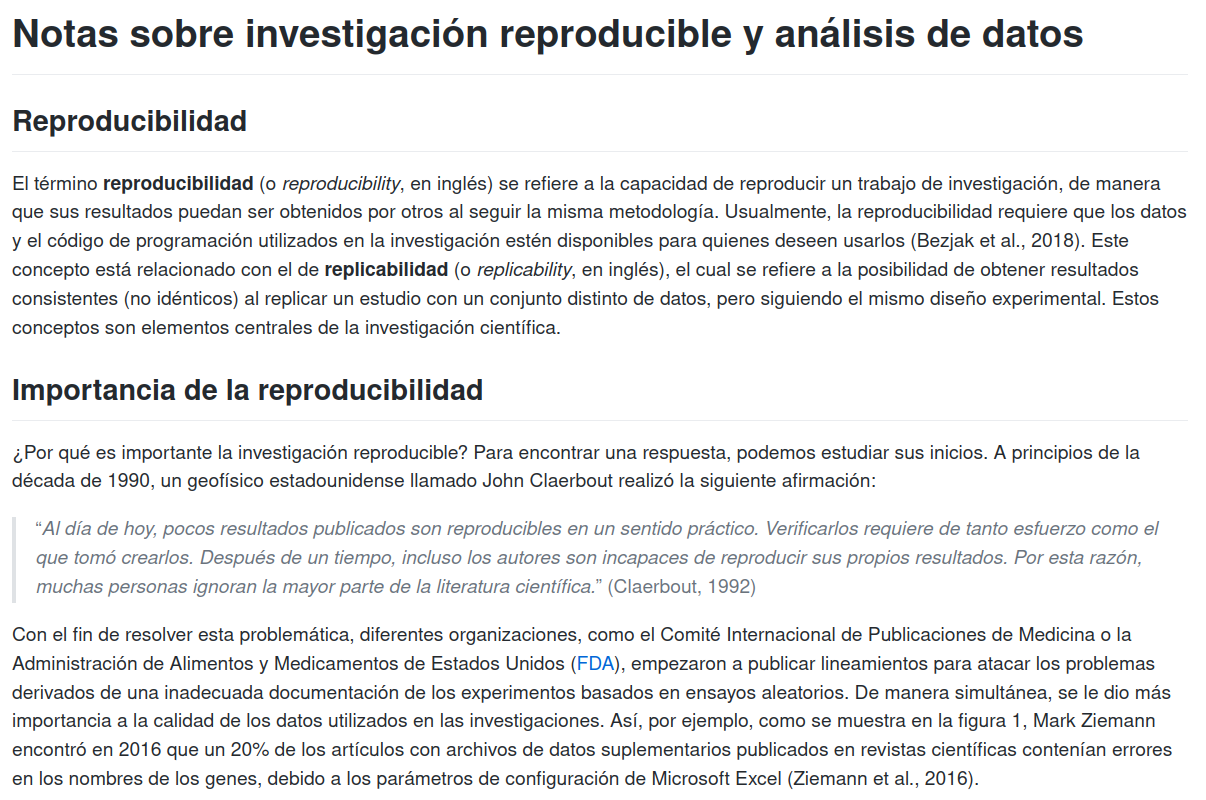
\includegraphics[width=4.02in,height=\textheight]{./img/tarea-01-img-01.png}

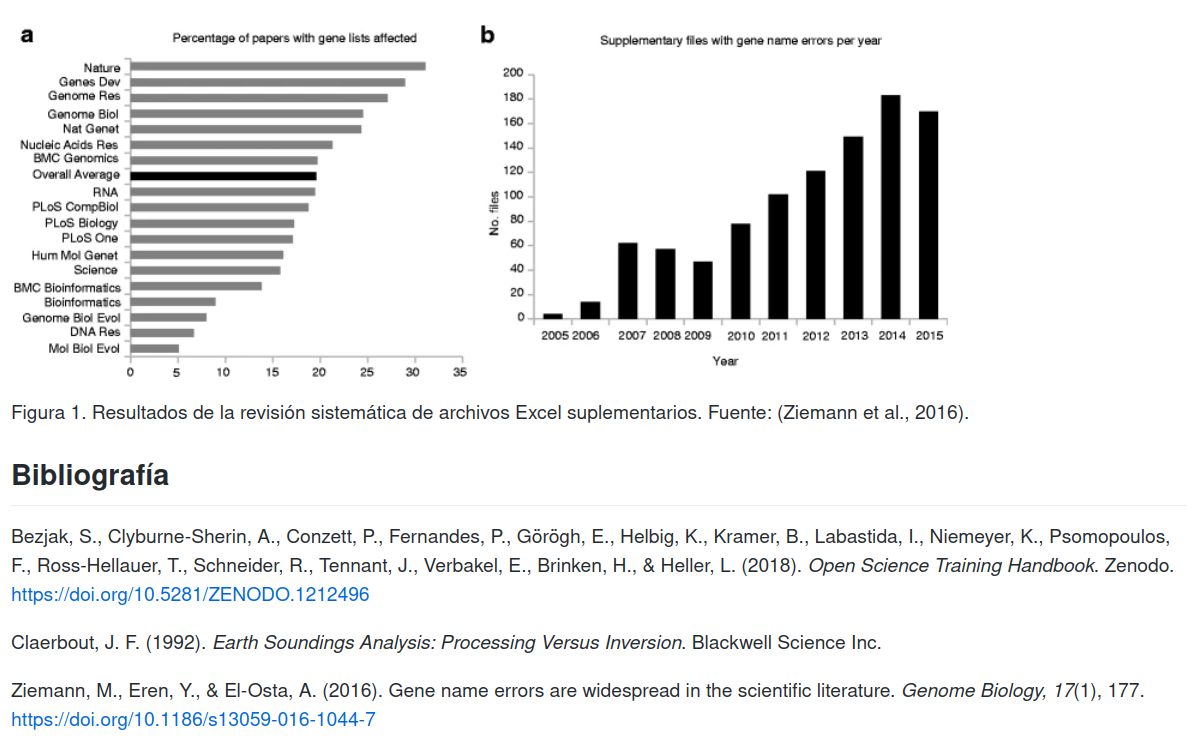
\includegraphics[width=4.01in,height=\textheight]{./img/tarea-01-img-02.png}

Los textos están disponibles en \href{otros/tarea-01-texto.txt}{este
enlace}.

\hypertarget{calificaciuxf3n}{%
\section*{Calificación}\label{calificaciuxf3n}}
\addcontentsline{toc}{section}{Calificación}

Entre paréntesis, se muestra el porcentaje correspondiente a cada
aspecto que se calificará:

Revisión de las direcciones entregadas:\\
- (5\%) Dirección del repositorio en GitHub.\\
- (5\%) Dirección del sitio web publicado en GitHub Pages.

Revisión de los elementos del documento escrito en Markdown:\\
- (10\%) Encabezados.\\
- (20\%) Negritas e itálicas.\\
- (20\%) Citas textuales.\\
- (20\%) Imagen de la figura 1 (el archivo está en
\href{img/ZiemannEtAlFig1.png}{ZiemannEtAlFig1.png}.\\
- (20\%) Hipervínculos (además de los dos de la bibliografía, incluya
uno al sitio web de la FDA en https://www.fda.gov/, en donde se
mencionan las siglas).

\hypertarget{examen-corto-02}{%
\chapter*{Examen corto 02}\label{examen-corto-02}}
\addcontentsline{toc}{chapter}{Examen corto 02}

\hypertarget{fecha-1}{%
\section*{Fecha}\label{fecha-1}}
\addcontentsline{toc}{section}{Fecha}

Lunes 10 de octubre de 2022

\hypertarget{temas-a-evaluar-1}{%
\section*{Temas a evaluar}\label{temas-a-evaluar-1}}
\addcontentsline{toc}{section}{Temas a evaluar}

\begin{itemize}
\tightlist
\item
  \href{https://pf0953-programacionr.github.io/2022-ii/05-r-conceptos_basicos.html}{R
  - conceptos básicos}
\end{itemize}

\bookmarksetup{startatroot}

\hypertarget{referencias-bibliogruxe1ficas}{%
\chapter*{Referencias
bibliográficas}\label{referencias-bibliogruxe1ficas}}
\addcontentsline{toc}{chapter}{Referencias bibliográficas}

\hypertarget{refs}{}
\begin{CSLReferences}{1}{0}
\leavevmode\vadjust pre{\hypertarget{ref-gandrud_reproducible_2020}{}}%
Gandrud, Christopher. 2020. \emph{Reproducible Research with {R} and
{RStudio}}. Third edition. The {R} Series. Boca Raton, FL: CRC Press.

\leavevmode\vadjust pre{\hypertarget{ref-longley_geographic_2005}{}}%
Longley, Paul A., Michael F. Goodchild, David J. Maguire, and David W.
Rhind. 2005. \emph{Geographic {Information} {Systems} and {Science}}.
2nd edition. Chichester ; Hoboken, NJ: Wiley.

\leavevmode\vadjust pre{\hypertarget{ref-olaya_sistemas_2020}{}}%
Olaya, Víctor. 2020. {``Sistemas de {Información} {Geográfica}.''}
\url{https://volaya.github.io/libro-sig/}.

\leavevmode\vadjust pre{\hypertarget{ref-peng_reproducible_2011}{}}%
Peng, Roger D. 2011. {``Reproducible {Research} in {Computational}
{Science}.''} \emph{Science} 334 (6060): 1226--27.
\url{https://doi.org/10.1126/science.1213847}.

\leavevmode\vadjust pre{\hypertarget{ref-singleton_establishing_2016}{}}%
Singleton, Alex David, Seth Spielman, and Chris Brunsdon. 2016.
{``Establishing a Framework for {Open} {Geographic} {Information}
Science.''} \emph{International Journal of Geographical Information
Science} 30 (8): 1507--21.
\url{https://doi.org/10.1080/13658816.2015.1137579}.

\end{CSLReferences}



\end{document}
